% !TEX program = xelatex
\documentclass[12pt]{article}

% 1) Поля по ГОСТу
\usepackage[a4paper,
            left=3cm,
            right=1.5cm,
            top=1.5cm,
            bottom=1.5cm
           ]{geometry}

% 2) Кодировка и локализация
\usepackage[T2A]{fontenc} % Кодировка для кириллицы
\usepackage[utf8]{inputenc} % Кодировка исходного файла
\usepackage[russian]{babel} % Подключение русского языкапереносов (хотя babel часто справляется сам)

\usepackage{hyphenat}
\usepackage{fontspec}  
\setmainfont{Times New Roman}

% 4) Межстрочный интервал 1.5
\usepackage{setspace}
\onehalfspacing

% 5) Выравнивание по ширине
\usepackage{microtype}

% 6) Колонтитулы и нумерация: первая без числа, дальше — по центру
\pagenumbering{arabic}
\usepackage{fancyhdr}
\fancyhf{}
\fancyfoot[C]{\thepage}
\renewcommand{\headrulewidth}{0pt}
\renewcommand{\footrulewidth}{0pt}

% 7) Отступы вокруг рисунков и подписи
\usepackage{caption}
\usepackage{subcaption}
\setlength{\textfloatsep}{1.5\baselineskip} % текст ↔ плавающий объект
\captionsetup[figure]{
  skip=1\baselineskip,       % рисунок ↔ подпись
  justification=centering    % подпись по центру (одинарный интервал)
}
\captionsetup[subfigure]{labelformat=empty,labelsep=none}

\usepackage{titlesec}
% ставим точку после номера секции
\renewcommand\thesection{\arabic{section}.}

% формат для \section: точка вручную
\titleformat{\section}
  {\normalfont\Large\bfseries\centering} % жирный, центр
  {\thesection.}                          % точка здесь
  {1em}{}

% формат для \subsection: явно по центру и с точкой
\renewcommand\thesubsection{\arabic{section}.\arabic{subsection}}
\titleformat{\subsection}
  {\normalfont\large\bfseries\centering} % жирный, центр, чуть мельче
  {\thesubsection.}                       % здесь точка одна
  {1em}{}

\usepackage[
  labelsep=period,               % точка после «Таблица N»
  justification=centering,       % центрируем подпись
  singlelinecheck=false          % НЕ выравнивать однострочные влево
]{caption}

% форматируем \section: жирный, размер по умолчанию, по центру
\titleformat{\section}
  {\normalfont\Large\bfseries\centering} % стиль заголовка
  {\thesection}                          % метка (номер + точка)
  {1em}                                  % отступ между меткой и текстом
  {}                                     % код перед текстом

% абзацный отступ
\setlength{\parindent}{1.25cm}
\usepackage{indentfirst}

\usepackage[space]{grffile}
\usepackage{cite}
\usepackage{xcolor}
\usepackage{graphicx}
\usepackage{amsmath}
\usepackage[labelsep=period]{caption}
\usetikzlibrary{external}
\tikzexternalize[prefix=tikz/]

\begin{document}
\textbf{}

% Первая страница без номера
\begin{titlepage}
  \centering

  % ВЕРХНИЕ ТЕКСТЫ
    \begin{spacing}{1}
      {\bfseries
        Московский государственный университет имени~М.\,В.~Ломоносова\\[1ex]
        Физический факультет\\[1ex]
        Кафедра общей физики и волновых процессов\\[3cm]
      }
    \end{spacing}

  % ТИТУЛ
  \begin{spacing}{1}
      {\bfseries Курсовая работа}\\[0ex]
      {\bfseries на тему}\\[1ex]
      {Параллельное численное моделирование трёхкаскадного волоконного усилителя чипированных импульсов}\\[4cm]
  \end{spacing}

  % БЛОК ВЫПОЛНИЛ И РУКОВОДИТЕЛЬ
  \begin{tabular}{c}
    \bfseries Выполнил:\\
    \bfseries студент 525 группы\\
    {\bfseries Делекторский Н.\,Ю.}\\[1ex]
    \rule{6cm}{0.4pt}\\
    (подпись)\\[2em]

    \bfseries Научный руководитель:\\
    \bfseries к.\,ф.-м.\,н. Воронин А.\,А.\\[1ex]
    \rule{6cm}{0.4pt}\\
    (подпись)
  \end{tabular}

  \vfill

  % НИЖНИЙ ТЕКСТ
  Москва — 2025 г.

\end{titlepage}

\pagestyle{fancy}
\fancyhf{}
\fancyfoot[C]{\thepage}
\renewcommand{\headrulewidth}{0pt}
\renewcommand{\footrulewidth}{0pt}

\pagenumbering{arabic}
\setcounter{page}{2}

\tableofcontents
\clearpage

\section{Введение}
Актуальность темы исследования многокаскадных волоконных усилителей на основе иттербия определяется стремительным
развитием лазерных технологий, которые сегодня широко используются в науке и прикладных областях. Волоконные лазеры и
усилители, доппированные ионами иттербия $Yb^{3+}$ имеют высокий квантовый выход, отличное качество луча ($M^2 \approx 1$),
диапазон усиления около 1030-1080 нм и высокую стабильность работы \cite{High_Power_Fiber_Lasers:_A_Review}. Эти
характеристики делают иттербиевые лазеры перспективными для решения широкого круга задач в различных областях науки
и техники.

Иттербиевые лазеры и усилители активно применяются в биофотонике благодаря оптимальной длине волны около 1040–1060 нм,
позволяющей эффективно реализовать двухфотонную \cite{wang2019926, kim2012two, perillo2016deep, karpf2016two} и даже
трёхфотонную \cite{toda2017temporal, moritomo2020multi, klioutchnikov2023three} микроскопию. В частности, излучение
на длине волны около 1050–1060 нм обеспечивает глубокое проникновение в биологические ткани до нескольких миллиметров
при минимальном повреждении клеток, что особенно важно для флуоресцентной визуализации и хирургии сверхкороткими
импульсами \cite{horton2013vivo, zipfel2003nonlinear}.

В области генерации и применения суперконтинуума волоконные системы на основе иттербия служат источниками
ультраширокополосного когерентного излучения (450-2000 нм), незаменимого в спектроскопии высокого разрешения
и метрологии \cite{dudley2006supercontinuum}.
В частности, они позволяют обнаруживать ткани, богатые липидами,
полоса которых находится вблизи 1720 нм. Солитонные режимы в иттербиевых волоконных лазерах реализуются в виде
диссипативных солитонов, стабилизируемых
балансом между дисперсией, нелинейностью, усилением и потерями. Эти режимы используются для генерации ультракоротких
импульсов высокой мощности и сложных структур, таких как \("\)солитонные молекулы\("\)
\cite{grelu2012dissipative, grelu2024solitary}. Самосдвиг частоты солитона, обусловленный комбинационным рассеянием,
приводит к сдвигу спектра в красную область и
позволяет получить импульсы с длинами волн, выходящими за пределы ширины усиления активной среды
\cite{han2021spectral}. Самокомпрессия импульсов в волокнах с аномальной дисперсией обеспечивает сокращение
длительности импульсов до десятков фемтосекунд, исключая необходимость внешних компрессоров
\cite{gaida2015self, giree2015high}.

Использование иттербиевых волокон с аномальной дисперсией (например, фотонных кристаллических волокон типа NL-PM750)
позволяет формировать короткие импульсы \cite{zhang2013sub, kurita2011dispersion, hou2018sub} и импульсы с энергиями
порядка 500 мкДж
\cite{tavella2010fiber}.

Кроме того, иттербиевые лазеры широко используются в квантовой оптике и атомной физике, обеспечивая необходимые
параметры излучения для охлаждения и захвата атомов, манипуляции с квантовыми состояниями и создания оптических
решёток \cite{ludlow2015optical}. Развитие высокоэнергетических многокаскадных усилителей позволяет существенно
увеличить доступные уровни энергии и мощности (пиковые мощности до нескольких гигаватт), открывая новые возможности
в области фундаментальных исследований и прецизионных измерений \cite{eidam2010fiber}.

В этой работе рассматривается модель оптической установки трёхкаскадного усилителя на основе иттербиевых волокон.
Выходная средняя мощность на уровне 1-2.5 Вт при частоте повторения 1 МГц и соответственно энергии импульса 1-2.5 мкДж
оптимальна для многофотонной микроскопии биотканей. Эта средняя мощность идеальна при использования полых волокон для
удержания моды. Однако реальные импульсы на выходе имеют пост- и предымпульсы. В данный
момент проблема решена, а цель этой работы — определить причины ухудшения импульса и предложить способы оптимизации установки.

\clearpage
\section{Описание модели}

На рисунке 1 приведена схема оптической установки, моделирование которой проводилось в этой работе. Номерами
обозначены элементы, которые были учтены при расчётах.

\begin{figure}[h]
    \centering
    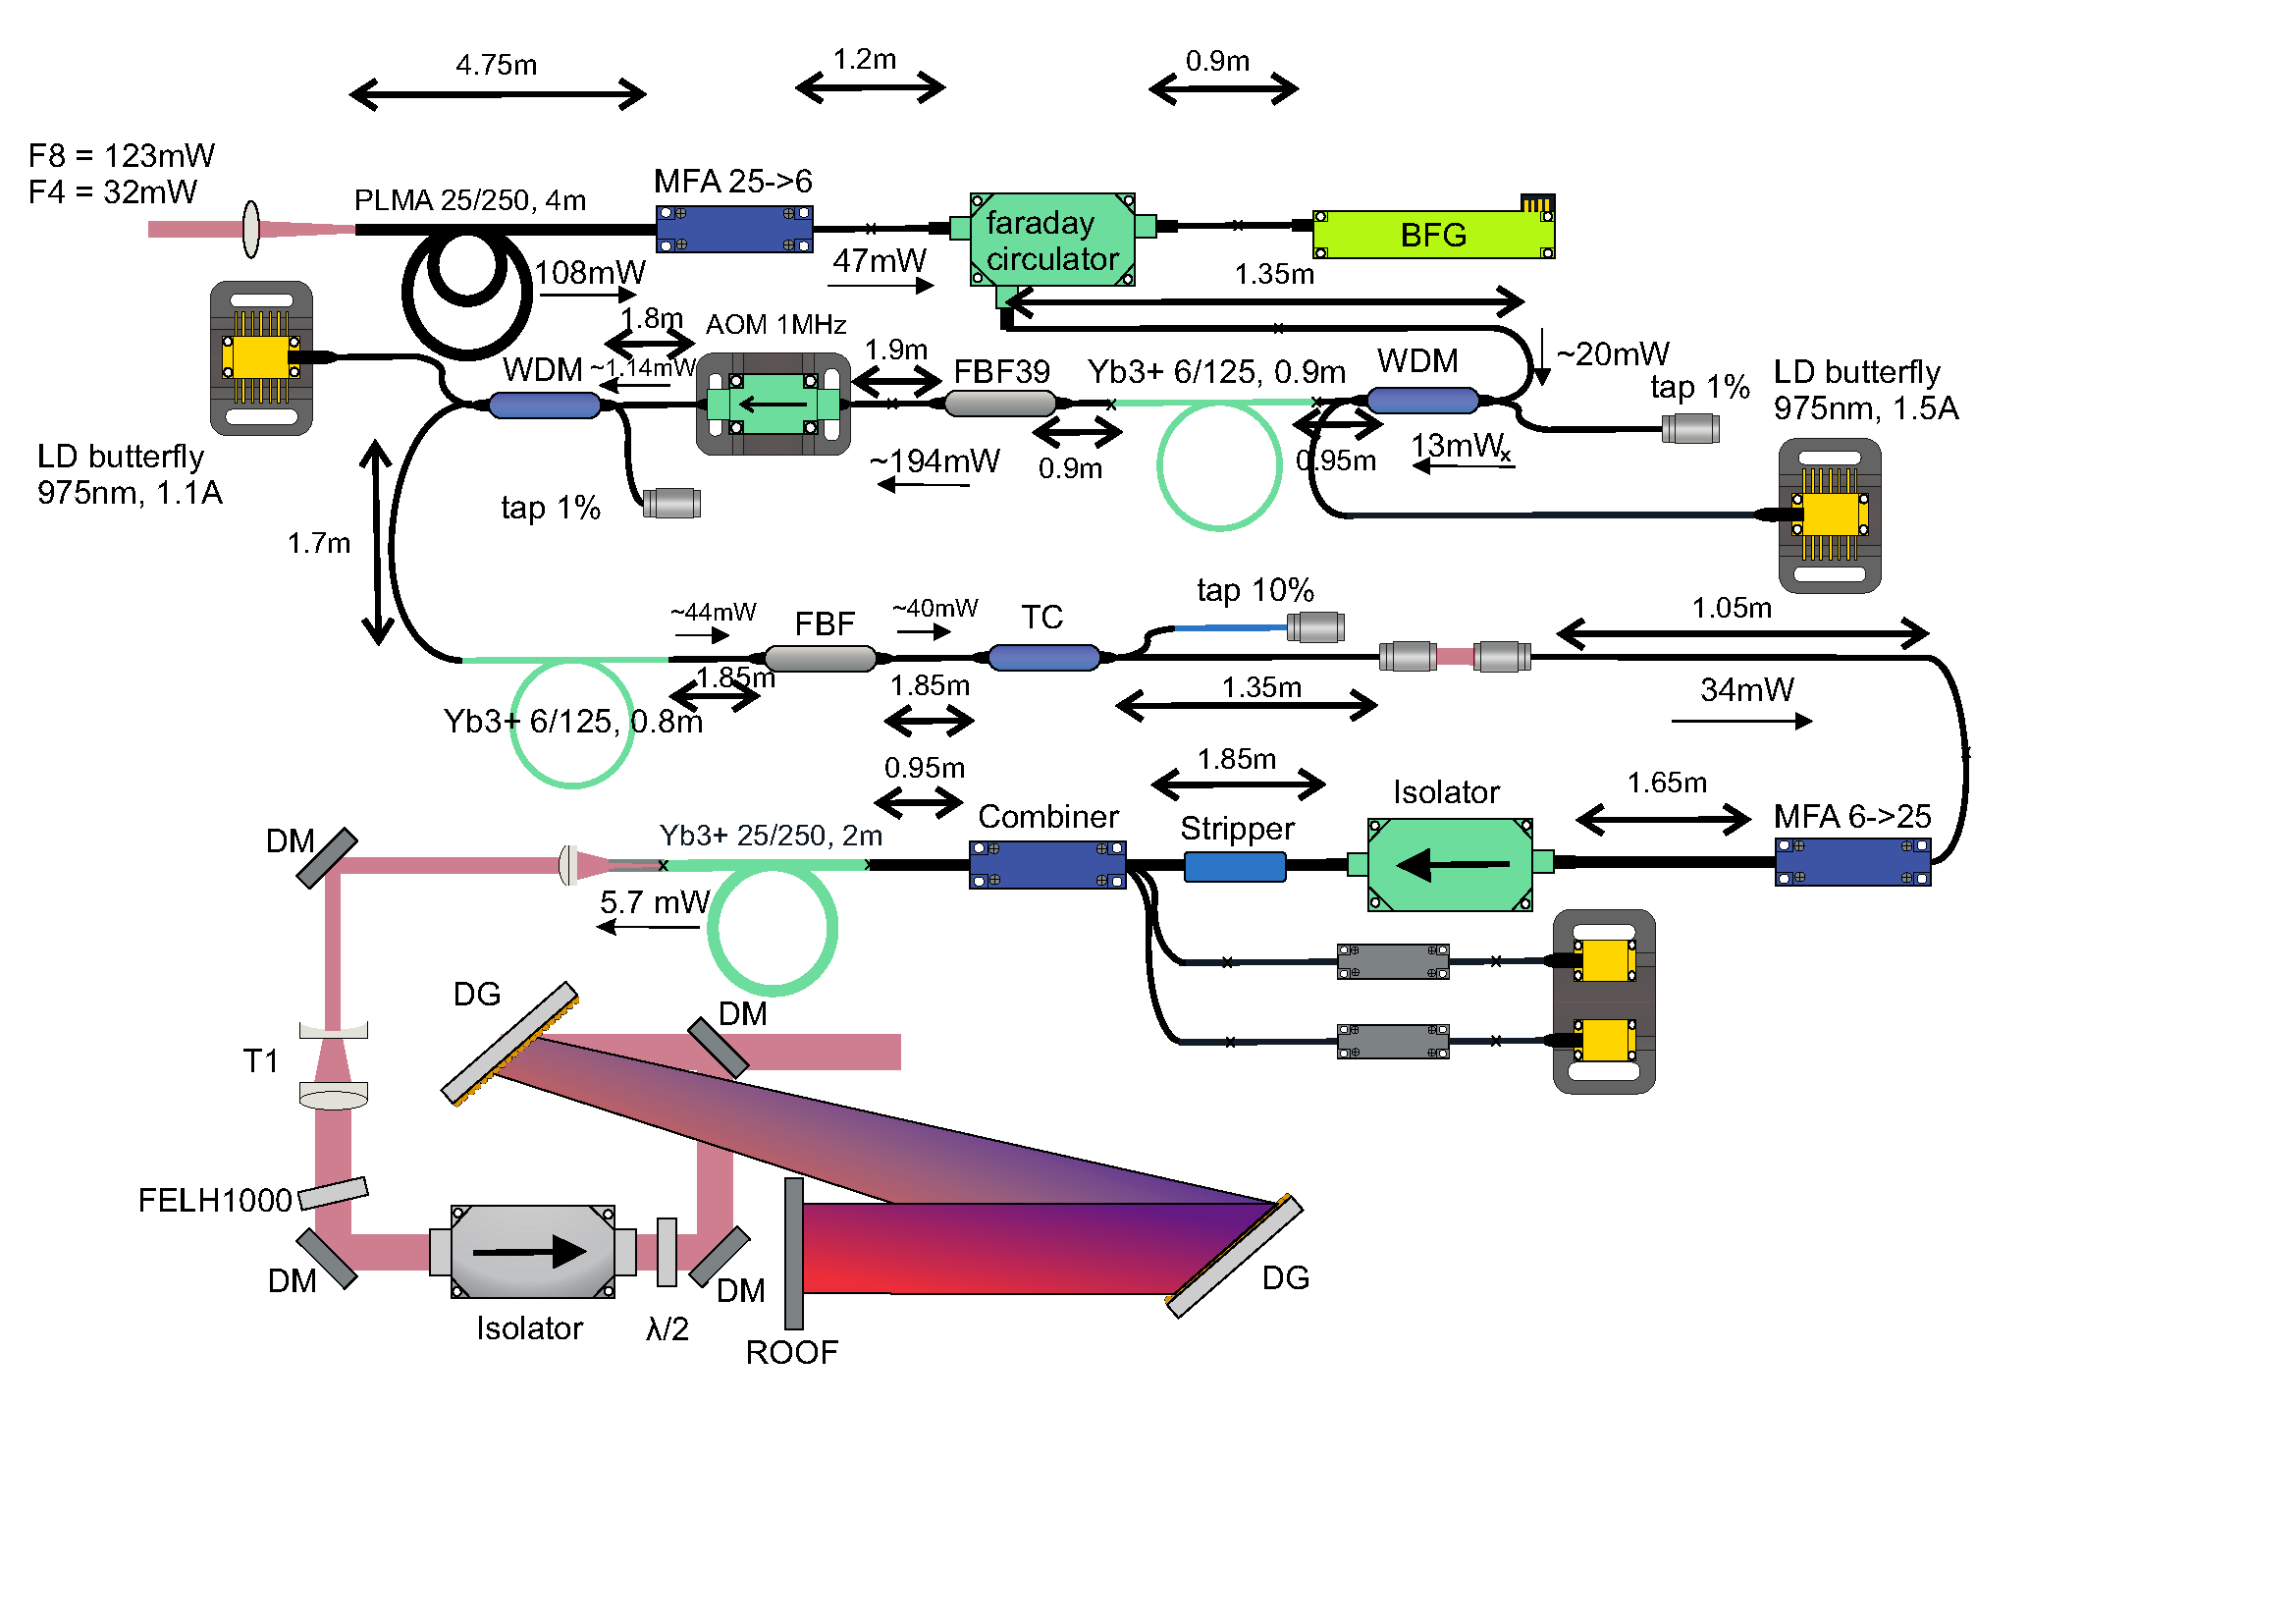
\includegraphics[trim=0 100 0 0, width=1\textwidth]{Images/YB_Amplifier_tech_data_sheme.png}
    \caption{Схема оптической установки. Числами обозначены элементы, которые используются в моделировании}
    \label{fig:rotated}
\end{figure}

\begin{figure}[h!]
    \centering
    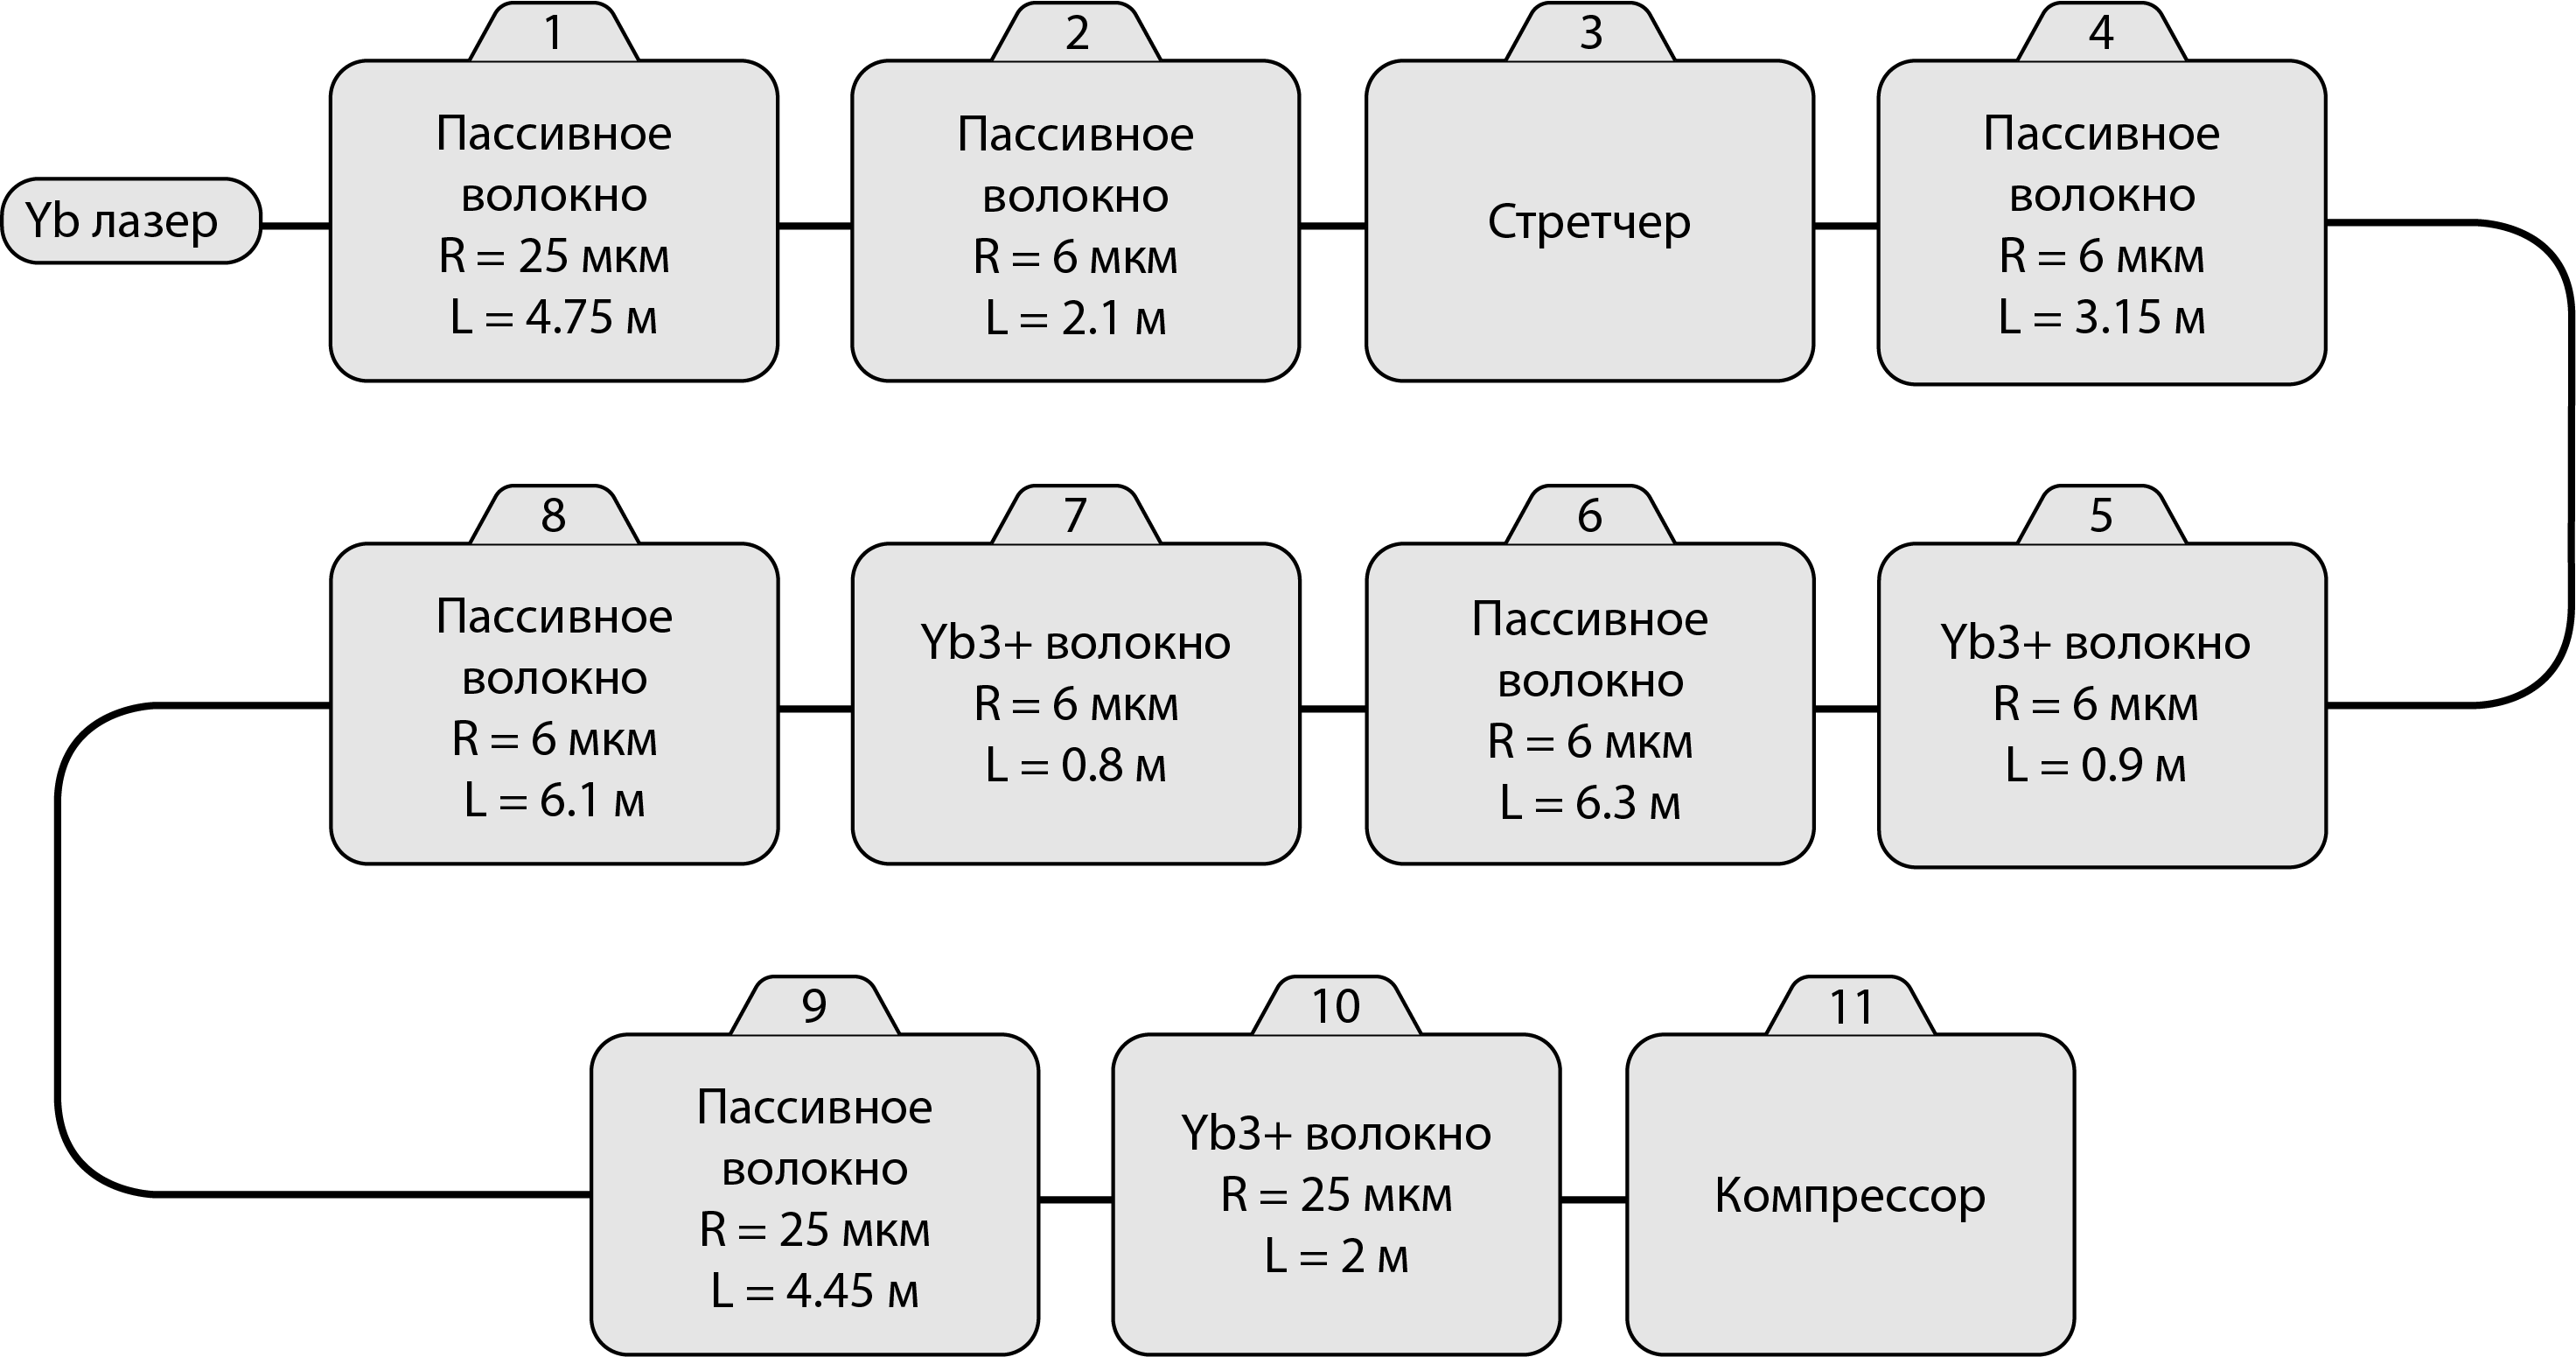
\includegraphics[width=1\textwidth]{Images/Оптическая установка.png}
    \caption{Упрощённая схема оптической установки. Числами обозначены элементы, которые используются в моделировании}
    \label{fig:rotated}
\end{figure}

Чёрным обозначены пассивные волокна, зелёным цветом выделены иттербиевые. Под номером 4 находится брэгговская
чирпированная решётка, под номером 24 - решёточный компрессор. Ниже будут подробнее рассмотрены модели элементов,
которые были использованы в моделировании. Для начального состояния импульса бралось распределение Гаусса с
длительностью, приближенной к экспериментальной — приблизительно 210 фс. Представленная на рисунке 1 схема сложна для
анализа, поэтому на рисунке 2 представлена упрощённая схема моделирования инструментов.

Для моделирования на входе использовался гауссов импульс с длительностью по полувысоте 210 фс с нулевой фазой
на центральной длине волны 1058 нм. На рисунке 3 показано начальное состояние поля.

\subsection{Моделирование активных и пассивных волокон}

Распространение лазерных импульсов в волокне можно описать уравнением эволюции:

\begin{equation}
    i \frac{\partial E(z, t)}{\partial z} = \sum_{n=2}^{5} \frac{\beta_n}{n!} \frac{\partial^n E(z, t)}{\partial t^n} - \hat{\gamma}(\omega) |E(z, t)|^2 E(z, t),
\end{equation}

где $\beta_n = \frac{d^n k(\omega)}{d \omega^n}$ - коэффиент дисперсии $n$-ого порядка, $\sum_{n=2}^{5} \frac{\beta_n}{n!}$ - учёт
вклада 2-5 порядков дисперсии, $\hat{\gamma} |E|^2 E$ - фазовая самомодуляция:

\begin{equation}
    \hat{\gamma}(\omega) |E(z, t)|^2 E(z, t) = \mathcal{F}^{-1} \Bigl[ \gamma(\omega)\mathcal{F} \bigr[ |E(z, t)|^2 E(z, t) \bigr] \Bigr],
\end{equation}

где $\gamma(\omega)$ - коэффициент нелинейности. Переход в спектральное представление необходим, чтобы учесть дисперсию
нелинейности. Без её учёта $\gamma(\omega)$ теряет зависимость от частоты и становится константой. В активном волокне в уравнении
(1) появляется ещё один член:

\begin{equation}
    i \frac{\partial E(z, t)}{\partial z} = \sum_{n=2}^{5} \frac{\beta_n}{n!} \frac{\partial^n E(z, t)}{\partial t^n} - \hat{\gamma}(\omega) |E(z, t)|^2 E(z, t) +
    \hat{g}(\omega)E(z, t)
\end{equation}

$\hat{g}(\omega)E(z, t)$ - усиление внутри иттербиевого волокна:

\begin{equation}
    \hat{g}(\omega)E(z, t) = \mathcal{F}^{-1} \Bigl[ g(\omega)\mathcal{F} \bigr[ E(z, t) \bigr] \Bigr],
\end{equation}

где $g(\omega)$ представлен на рисунке 4. Выбор порядков дисперсии связан с тем, что для брэгговской волоконной решётки
производитель указал только эти порядки (таблица 1).

\begin{figure}[h]
    \centering
    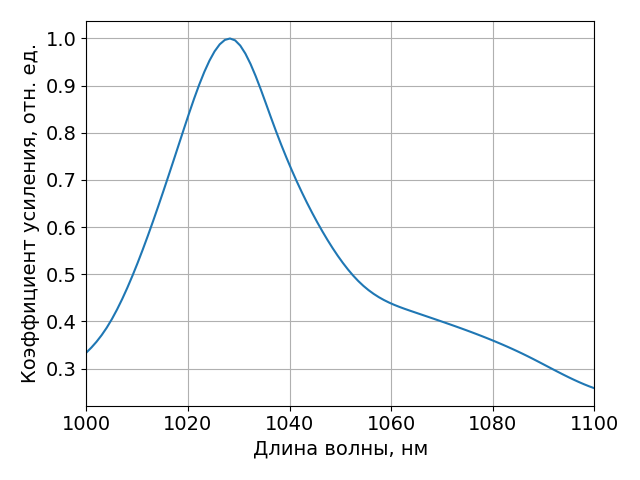
\includegraphics[trim=0 30 0 0, width=0.8\textwidth]{Images/Спектр усиления.png}
    \caption{Нормированный пектр усиления иттербия}
    \label{fig:rotated}
\end{figure}

В уравнении (1) можно обратить внимание, что дисперсионная составляющая может быть вычислена точно с использованием
Фурье-преобразования. Для численного решения остальной части уравнения был использован метод Рунге-Кутта 4-5 порядка.
Эти 2 способа решения были объеденены с помощью split-step метода. Так как дисперсионная часть вычисляется точно,
шаг интегрирования должен выбираться отсносительно фазовой самомодуляции. Максимальное изменение фазы можно оценить как:

\begin{equation}
    \varphi_{max} = \gamma P_0 z
\end{equation}

Шаг $h$ выбирался так, чтобы за него изменение фазы не превышало 0.01 радиан. Split-step метод подразумевает, что на
промежутке $h/2$ действует только дисперсия, а на второй половине шага — остальная часть уравнения.

\subsection{Чирпированная брегговская волоконная решётка}

Точная структура брэгговской решётки неизвестна, однако производитель приводит коэффициенты дисперсии, которые она
вносит. Они указаны в таблице 1.

\begin{figure}[h]
    \centering
    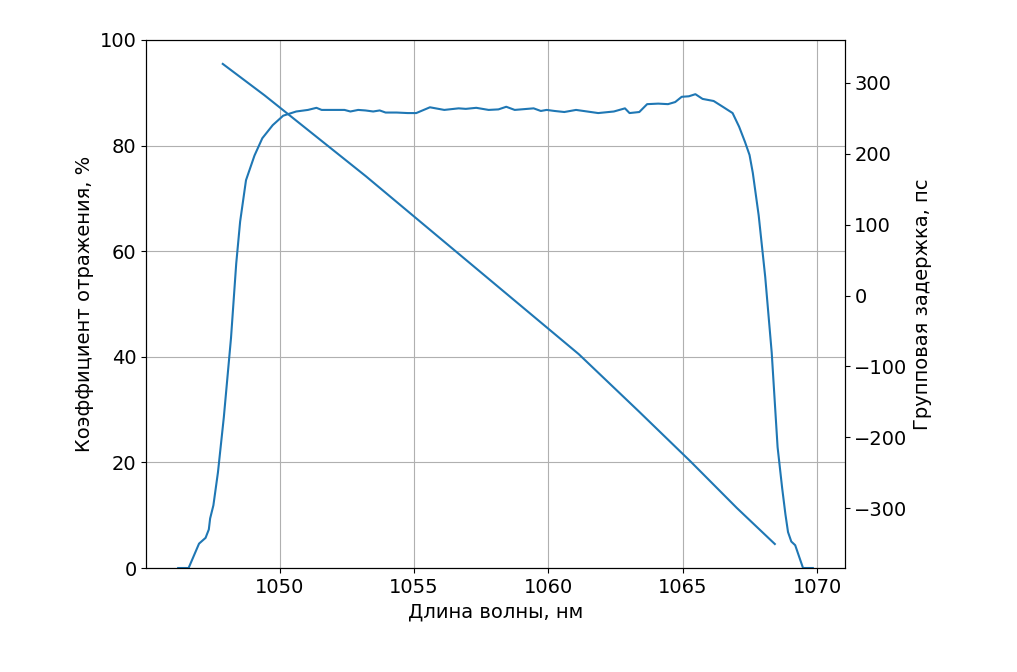
\includegraphics[trim=0 50 0 0, width=0.7\textwidth]{Images/Спектр решётки.png}
    \caption{Спектр и групповая задержка брэгговской чирпированной решётки}
    \label{fig:rotated}
\end{figure}

\begin{table}[h!]
    \centering
    \begin{tabular}{|c|c|}
        \hline
        $\beta_2$ & $19{.}28126~\text{пс}^2$ \\
        $\beta_3$ & $-0{.}16907~\text{пс}^3$ \\
        $\beta_4$ & $2{.}3141 \cdot 10^{-3}~\text{пс}^4$ \\
        $\beta_5$ & $-4{.}5379 \cdot 10^{-5}~\text{пс}^5$ \\
        \hline
    \end{tabular}
    \caption{Коэффициенты дисперсии чирпированной брэгговской решётки, предоставленные производителем}
    \label{tabюexample}
\end{table}

По этим коэффициентам можно восстановить фазу, которую решётка добавляет к импульсу:

\begin{equation}
    \varphi(\omega) = \sum_{n=2}^{5} \beta_n (\omega - \omega_0)^n
\end{equation}

Производитель также указал спектр пропускания решётки $R(\omega)$ (рисунок 5). Таким образом, прохождение импульса через
брэгговскую решётку можно описать уравнением:

\begin{equation}
    E(z, t) = \mathcal{F}^{-1} \Bigl[ \mathcal{F} \bigl[ E(z, t) \bigr] R(\omega) exp^{-i\varphi(\omega)} \Bigr],
\end{equation}

\begin{figure}[h!]
  \centering
  \begin{minipage}[b]{0.5\textwidth}
    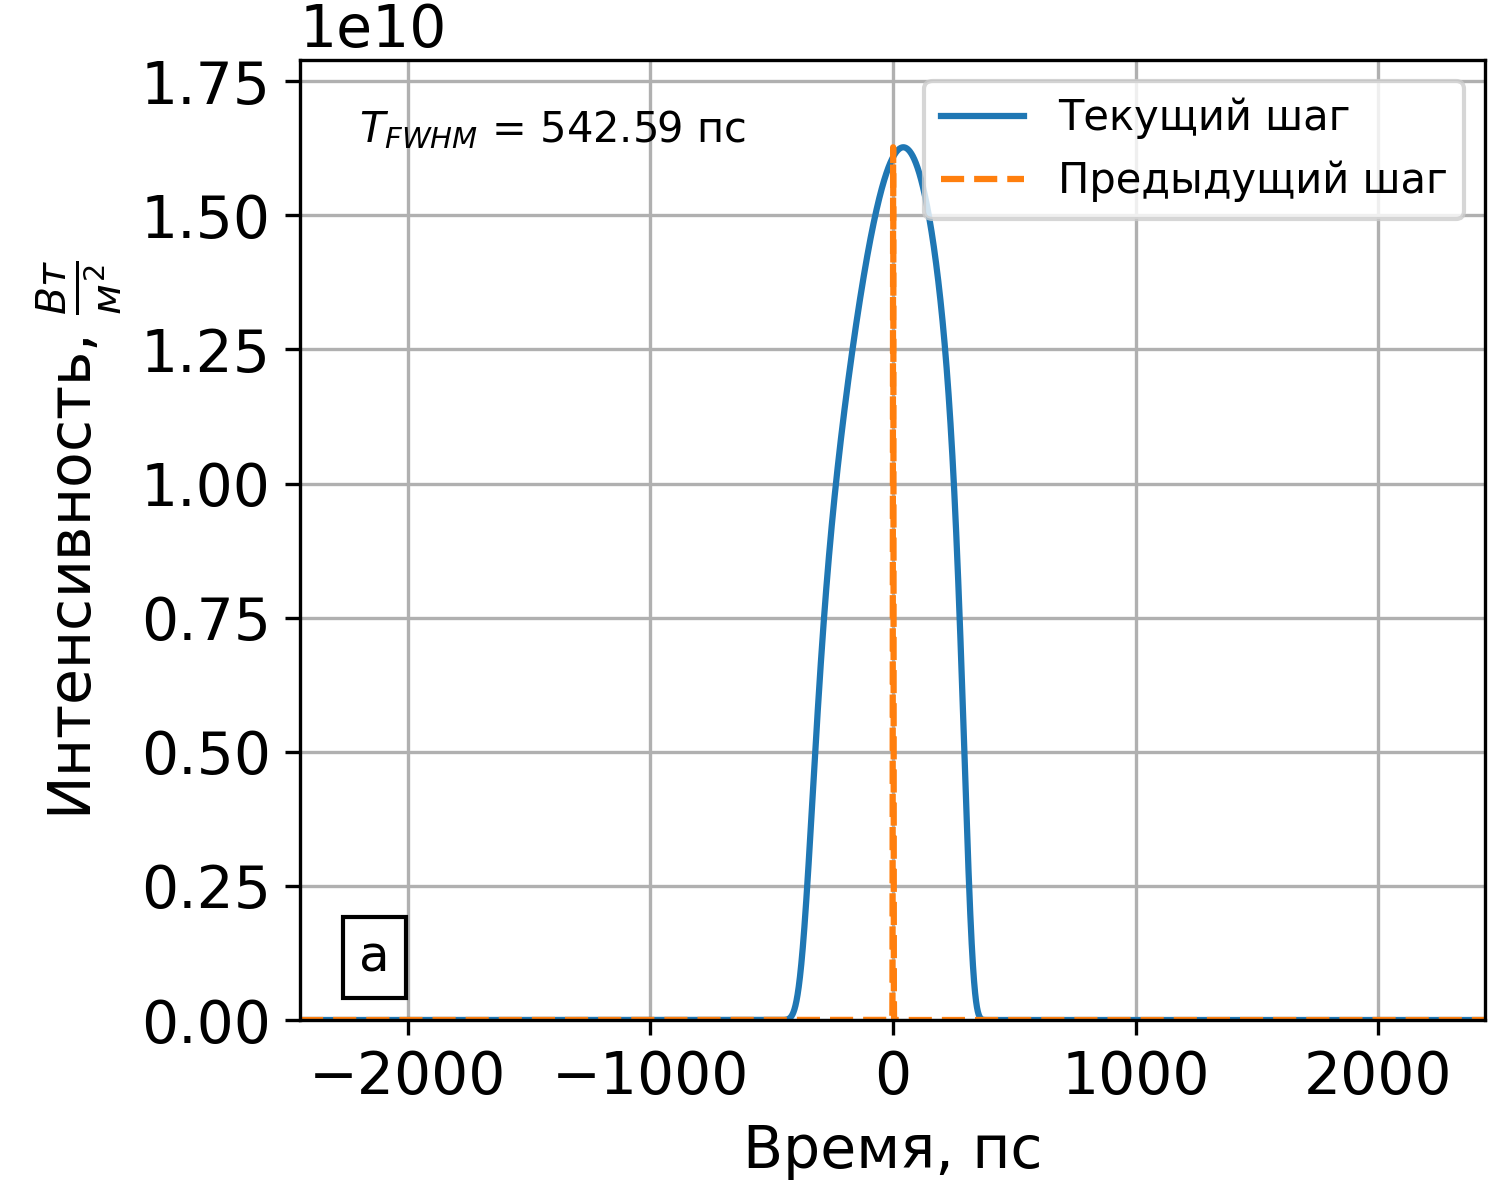
\includegraphics[width=\linewidth]{Images/Gauss Pulse/Импульс и спектр/!4. BFG_pusle}
  \end{minipage}% <- % убирает хвостовой пробел / перевод строки
  \begin{minipage}[b]{0.5\textwidth}
    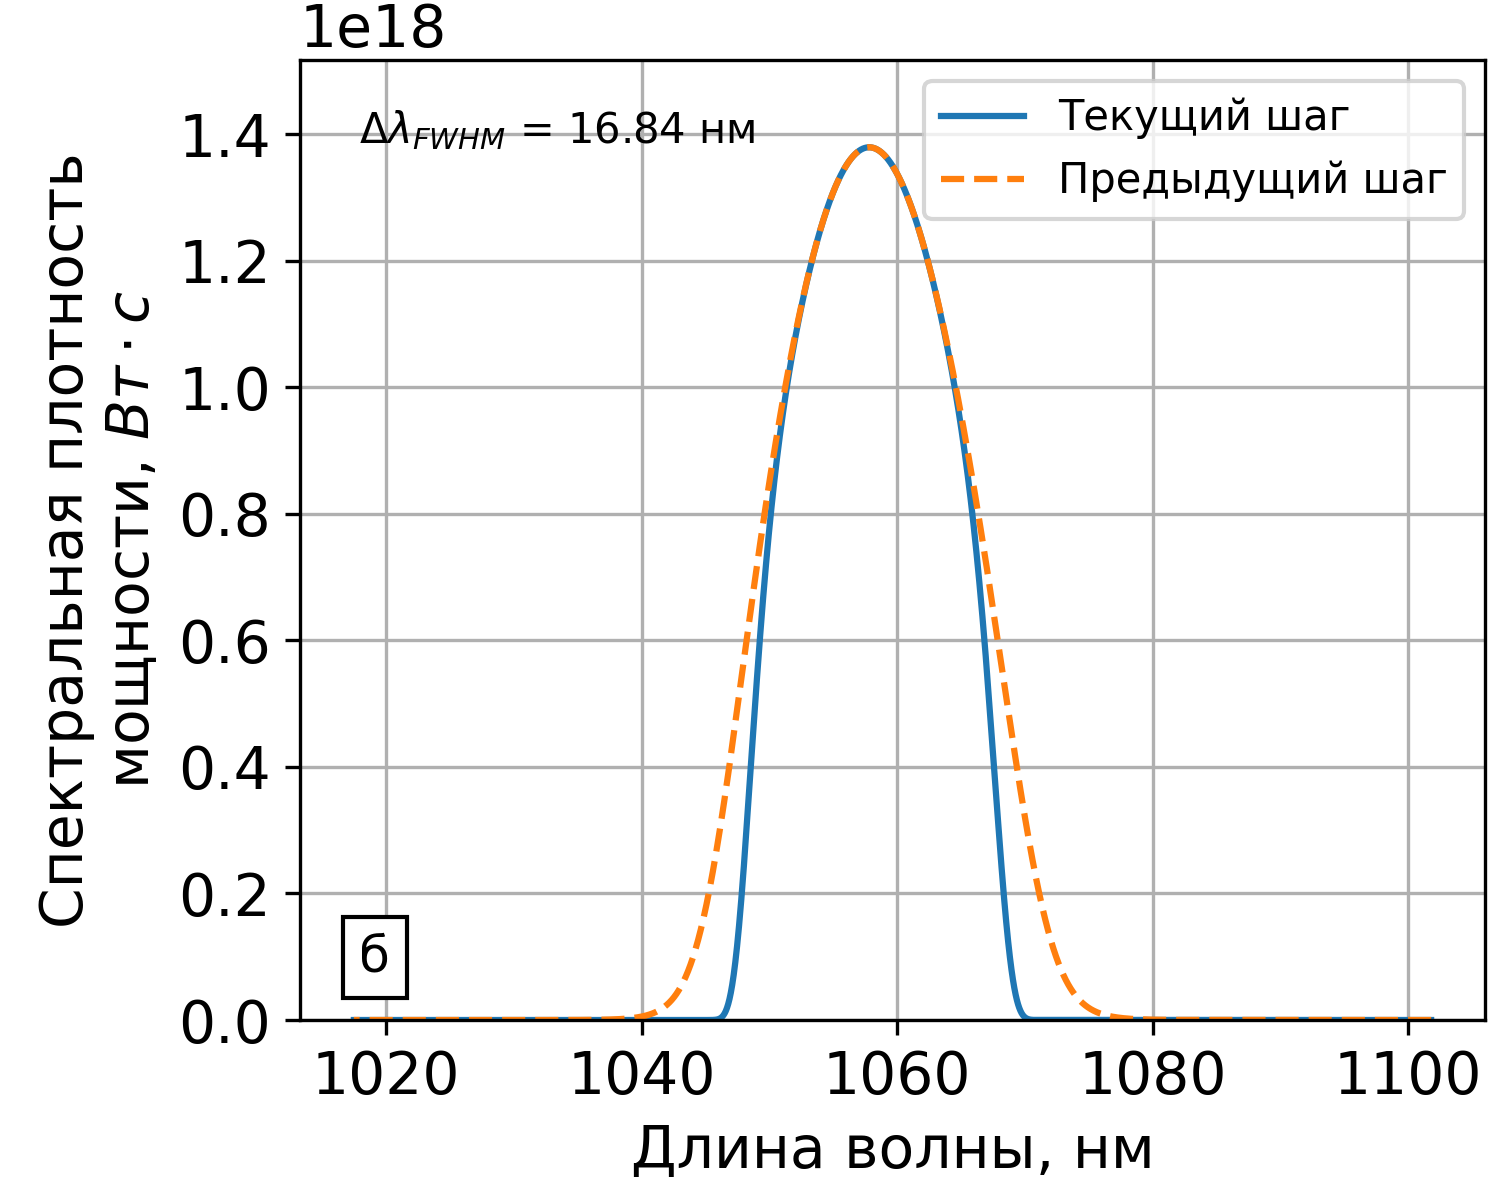
\includegraphics[width=\linewidth]{Images/Gauss Pulse/Импульс и спектр/!4. BFG_spectrum}
  \end{minipage}

  \vspace{}

  \begin{minipage}[b]{0.5\textwidth}
    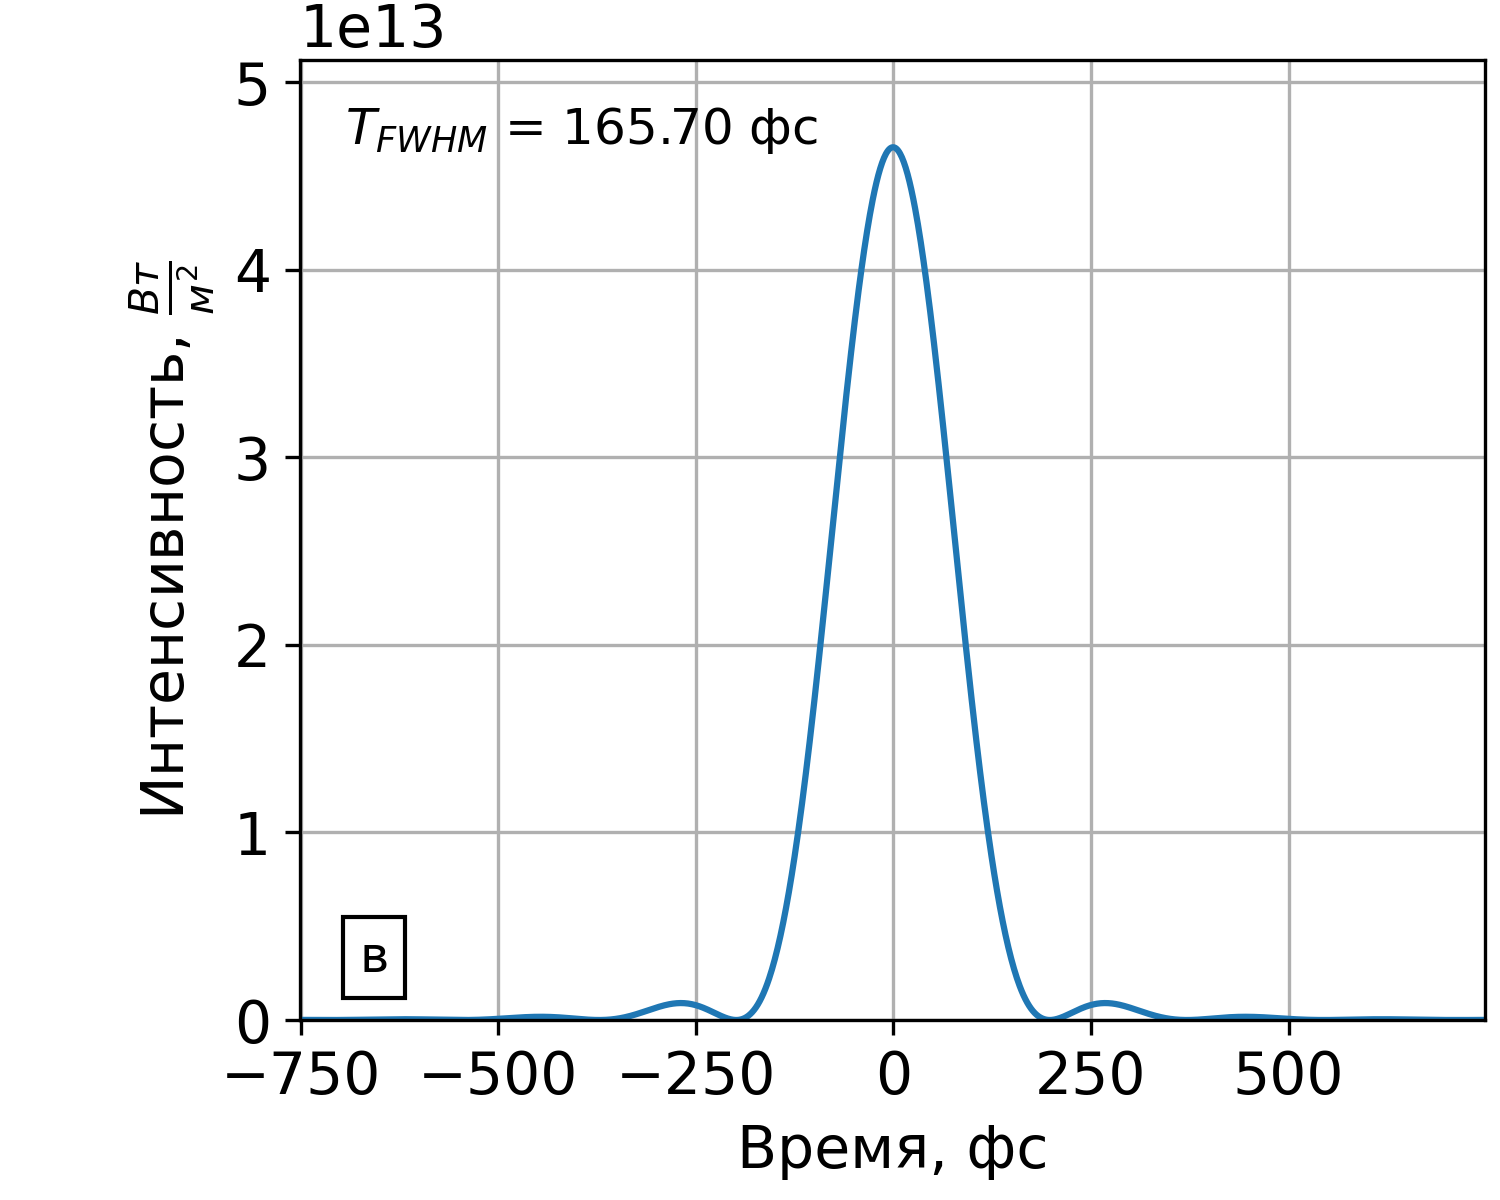
\includegraphics[width=\linewidth]{Images/Gauss Pulse/После компрессора/4 элемент gamma=49.41509 l_g=0.36344 сжатие}
  \end{minipage}% <- % убирает хвостовой пробел / перевод строки
  \begin{minipage}[b]{0.5\textwidth}
    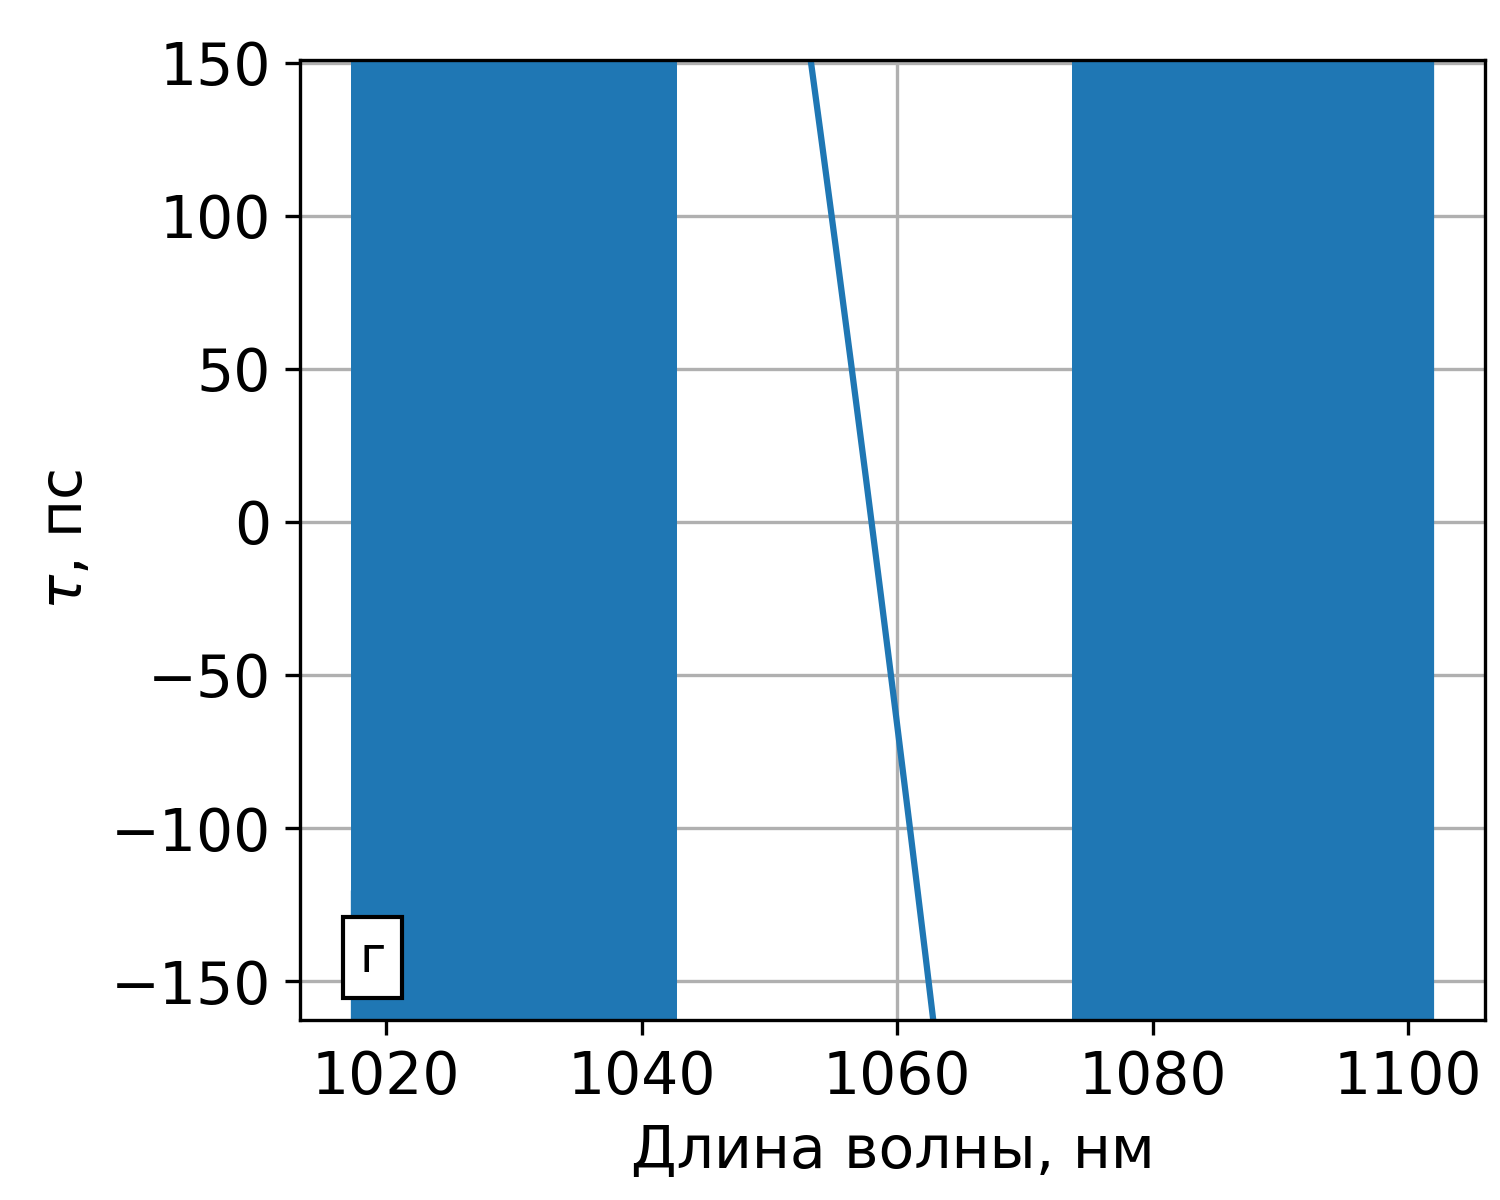
\includegraphics[width=\linewidth]{Images/Gauss Pulse/Импульс и спектр/!4. BFG_time_delay}
  \end{minipage}

  \caption{Состояние а) импульса, б) его спектра г) и групповой задержки после прохождения брэгговской решётки. Приведён
  график г) импульса, сжатого в решёточном компрессоре}
  \label{fig:both}
\end{figure}

Отдельно стоит отметить, что для моделирования растягивания импульса с 3 пс до почти 550 нужна большая сетка, которую
не оптимально использовать в моделировании волокон. Чтобы осуществить переход на большую сетку размером $2^{22}$ точек,
использовалась интерполяция комплексного массива поля для действительной и мномой частей отдельно. Выбирался другой
шаг по осям времени и, следовательно, частот, чтобы растяжение импульса было корректным. После прохождения брэгговской
решётки сетка снова приводилась к размеру $2^{18}$ точек.

На рисунке 5 показан результат моделирования брэгговской
решётки. Спектр отражения оказывается чуть уже, чем спектр импульса, поэтому происходит обрезание на краях. Импульс становится
немного не симметричным. Это сказывается на способности импульса к сжатию: на рисунке 5 г) видно появление пъедестала
после сжатия.

\subsection{Решёточный компрессор}

Для моделирования решёточного компрессора была использована формула \cite{wollenhaupt2007femtosecond} для описания
дисперсии второго порядка:

\begin{equation}
    \frac{d^2 \varphi(\omega)}{d\omega^2} = \beta_2(\omega) = -\frac{\lambda^3}{\pi c^2 d^2 \cos^2[\theta(\lambda)]} \, L,
\end{equation}

где $\theta(\lambda)$:

\begin{equation}
    \cos[\theta(\lambda)] = \sqrt{1 - \left( \frac{\lambda}{d} - \sin\gamma \right)^2},
\end{equation}

$\gamma$ - угол падения излучения на решётку, $L$:

\begin{equation}
    L = \frac{l_g}{\sqrt{1 - \left( \frac{\lambda}{d} - \sin(\gamma) \right)^2}},
\end{equation}

$l_g$ - расстояние между решётками. Так как брэгговская решётка вносит дисперию 2-5 порядков, уравнение 8 было
символьно продифференцировано, чтобы получить коэффициенты $\beta_2$ - $\beta_5$:

\begin{equation}
    \beta_3 = \frac{\partial \beta_2}{\partial \omega}
\end{equation}

\begin{equation}
    \beta_4 = \frac{\partial^2 \beta_2}{\partial \omega^2} + \Delta \beta_4
\end{equation}

\begin{equation}
    \beta_5 = \frac{\partial^3 \beta_2}{\partial \omega^3} + \Delta \beta_5,
\end{equation}

где $\Delta \beta_4$ и $\Delta \beta_5$ — поправки к коэффициентам. В ходе моделирования стало понятно, что для
решёточного компрессора взятие производных от $\beta_2$ до 5 порядка некорректно. В таком случае, по формуле (8),
получается зависимость только от двух параметров $\gamma$ и $l_g$, что не отражает вклад 4 и выше порядков. Так как
компрессор компенсирует чирп, то его коэффициенты отличаются знаком от чисел стретчера, поэтому формула остаётся
похожей на (7):

\begin{equation}
    E(z, t) = \mathcal{F}^{-1} \Bigl[ \mathcal{F} \bigl[ E(z, t) \bigr] exp^{-i\varphi(\omega)} \Bigr]
\end{equation}

\subsection{Оптимизация вычислений}

Для моделирования использовался компьютер с процессором AMD Ryzen 7 5800X, видеокартой Nvidia GeForce RTX 4060 Ti.
Использовался язык программирования Python. Сам по себе он довольно медленный в расчётах, однако он позволяет
управлять скриптами для быстрой математики посредством библиотеки NumPy, написанная на C для большей части операций
и Fortran для линейной алгебры, что позволяет векторизировать операции и избегать прямого использования Python
в расчётах. Хотя скорость языка C практически близка к предельно возможной, некоторые операции можно ускорить
с использованием параллельного программирования.

Для распраллеливания основной критерий — независимость мелких вычислений внутри одной крупной, так как отдельные
потоки не \("\)знают\("\), что делают соседние, поэтому при несоблюдении правила результат может быть непредсказуем.
При этом крупная операция должна быть достаточно сложной, чтобы распределение ресурсов между потоками не занимало
больше времени, чем выполнение самой задачи. Основным кандидатом на распараллеливание является преобразование Фурье:

\begin{equation}
    X_k
    =\sum_{n=0}^{N-1}\hat{x}_n\,e^{-2\pi i\frac{k\,n}{N}},
    \quad k=0,1,\dots,N-1.
    \label{eq:equation}
\end{equation}

Как видно из формулы (12), каждый член выражения независим от других, поэтому сумму можно считать частями параллельно.
Стандартная однопоточная реализация на C даёт $12.682 \pm 0.014$ мс на операцию
$\mathcal{F}^{-1} \Bigl[ \mathcal{F} \bigl[ x \bigr] \Bigr]$ c комплексным массивом $x$ длиной $2^{18}$ элементов.
Все тесты запускались 30 раз по 1000 массивов, чтобы исключить влияние случайных факторов. При расчёте эволюции поля
в пассивном волокне эта операция выполняется 2 раза на каждом шаге интегрирования, в иттербиевом — 3 раза, что
довольно сильно влияет на общую производительность.

Для распараллеливания можно использовать библиотеку FFTW для C. Тот же тест показывает $593 \pm 3$ мкс на одну
операцию, что даёт выигрыш больше, чем в 20 раз. Процессор, на котором выполнялся расчёт, имеет 8 логических ядер.
Соответственно при увеличении их количества время выполнения преобразования будет расти до тех пор, пока накладные
ресурсы на распараллеливание не превысят время суммирования. Однако даже очень мощные серверные решения имеют обычно
не больше 64 ядер. В то же время в современных видеокартах могут быть тысячи и даже десятки тысяч CUDA-ядер.

Для сравнения в видеокарте, которая использовалась в расчётах, для преобразования выше использовались 4864 ядра,
которые выполняли его в среднем за $502.6 \pm 3$ мкс. Это даёт выигрыш в 25 раза по сравнению с однопоточной
реализацией и примерно в 1.2 раза по сравнению с параллельной версией на процессоре.

\begin{figure}[h]
    \centering
    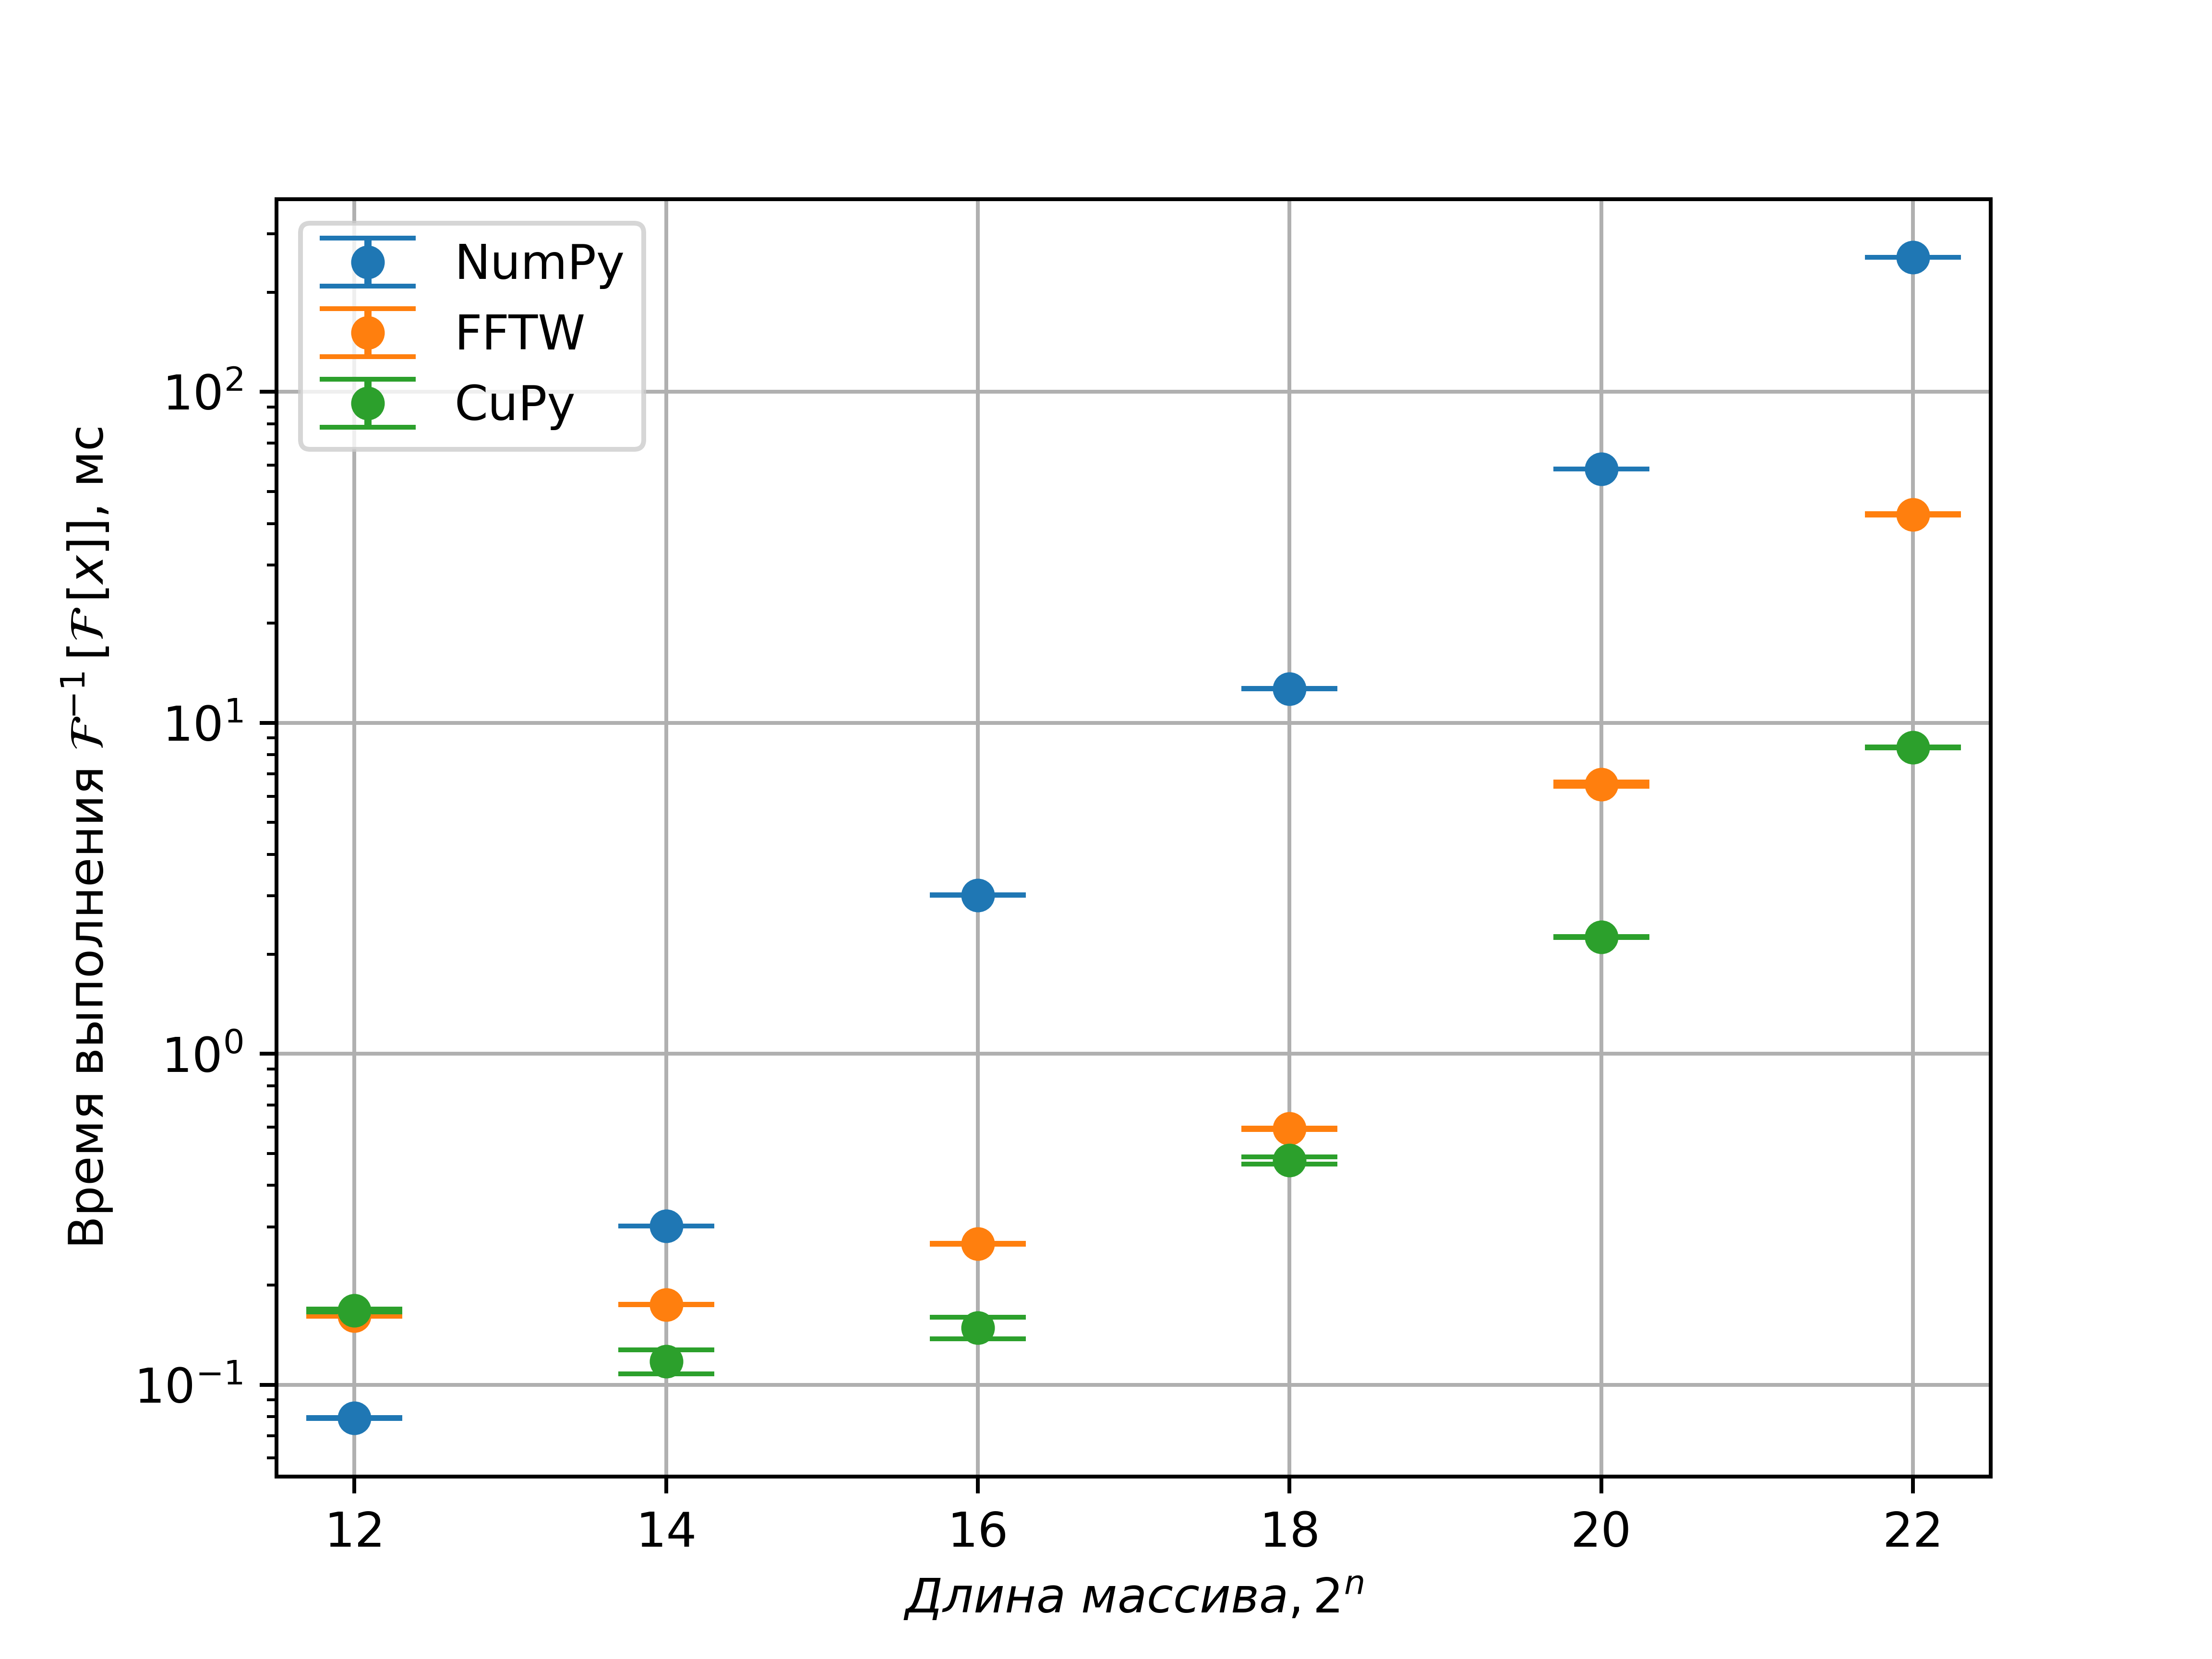
\includegraphics[trim=0 0 0 0, width=0.8\textwidth]{Images/Время выполнения}
    \caption{Время выполнения операции $\mathcal{F}^{-1} \Bigl[ \mathcal{F} \bigl[ x \bigr] \Bigr]$ для массивов разной длины. NumPy реализует однопоточные операции, FFTW распараллеливает оперции на ядра процессора, CuPy распараллеливает на видеокарте}
    \label{fig:rotated}
\end{figure}

На рисунке 6 представлены времена выполнения выше указанных операций. На нём видно, что для комплексных массивов
длиной $2^{12}$ элементов, как и для меньших, распараллеливание не имеет никакого смысла, потому что накладные
расходы превышают выигрыш. Однако при увеличении длины массива выигрыш становится существенным.

Для другого примера рассмотрим скалярное умножение комплексных массивов длиной $2^{18}$ элементов. Эта операция
очень простая, поэтому накладные расходы на распараллеливание превышают время выполнения однопоточной реализации.
Но при этом расчёт на процессоре занимает $849.0 \pm 1.6$ мкс, а на видеокарте $24.27 \pm 0.25$ мкс. Разница примерно
в 20 раз объясняется пропускной способностью оперативной памяти в случае процессора и шины в случае видеокарты,
но вычисление во втором случае оказывается намного более выгодным.

Однако вся последующая обработка данных должна выполняться на процессоре, поэтому важно рассмотреть канал передачи
информации между процессором и видеокартой. В используемой модификации компьютера они соединены через шину PCI
Express 4.0 по 16 линиям связи. Этот стандарт обеспечивает скорость передачи данных до 32 Гб/с. Используемый выше
массив комплексных чисел занимает 4 Мб памяти. Это означает, что в лучшем случае на передачу его от процессора
видеокарте и обратно нужно примерно 0.24 мс. Поэтому частный обмен данными между процессором и видеокартой может
существенно замедлять расчёт. Для комплексного массива длиной $2^{22}$ время возрастает уже почти до 4 мс.

Размеры массивов в примерах соответствуют используемым в моделировании. К примеру, на брэгговской решётке импульс
растягивается с 4 до 500 пс. При этом для избежания артефактов счёта на изначальный импульс выбирается не меньше
100 точек по полувысоте. При этом временная и частотная оси связаны уравнением:

\begin{equation}
    N_t = \frac{2\pi}{\Delta \omega \Delta \tau},
\end{equation}

где $N_t$ — количество точек. Для охвата и временной, и частотной осей при моделировании брэгговской решётки и
компрессора используются массивы размерами $2^{22}$ точек. Временная ось охватывает масштаб 5 нс, что позволяет избежать
артефактов Фурье-преобразования. При этом обеспечивается достаточная точность для описания импульса до рястяжения.
В волокнах, если влияние дисперсии и фазовой самомодуляции на импульс незначительно, произвоится переход на сетку
$2^{16}$ точек. В противном случае используется сетка $2^{18}$ точек.

\clearpage
\section{Результаты}

Ниже представлены результаты моделирования. После растягивания импульса на чирпированной брэгговской решётке
будет приводиться моделирование решёточного компрессора сразу после этого элемента для более наглядного
представления изменений.

\subsection{Моделирование гауссова импульса со спетром усиления Yb3+}

На рисунке 7 графики импульса (рисунок 7а) после первого каскада усиления (номер 5 на рисунке 2). Спектр усиления
$Yb^{3+}$ (рисунок 7б) приводит к появлению сильной асимметрии на спектре и, следовательно, на импульсе. На рисунке 7в
представлен импульс компрессора. На нём видно, что пъедестал стал больше, а длительность импульса увеличилась.
На графике спектра изображён профиль,полученный в эксперименте. Он был использован для подбора параметров спектра
усиления $Yb^{3+}$.

\begin{figure}[h!]
  \centering
  \begin{minipage}[b]{0.5\textwidth}
    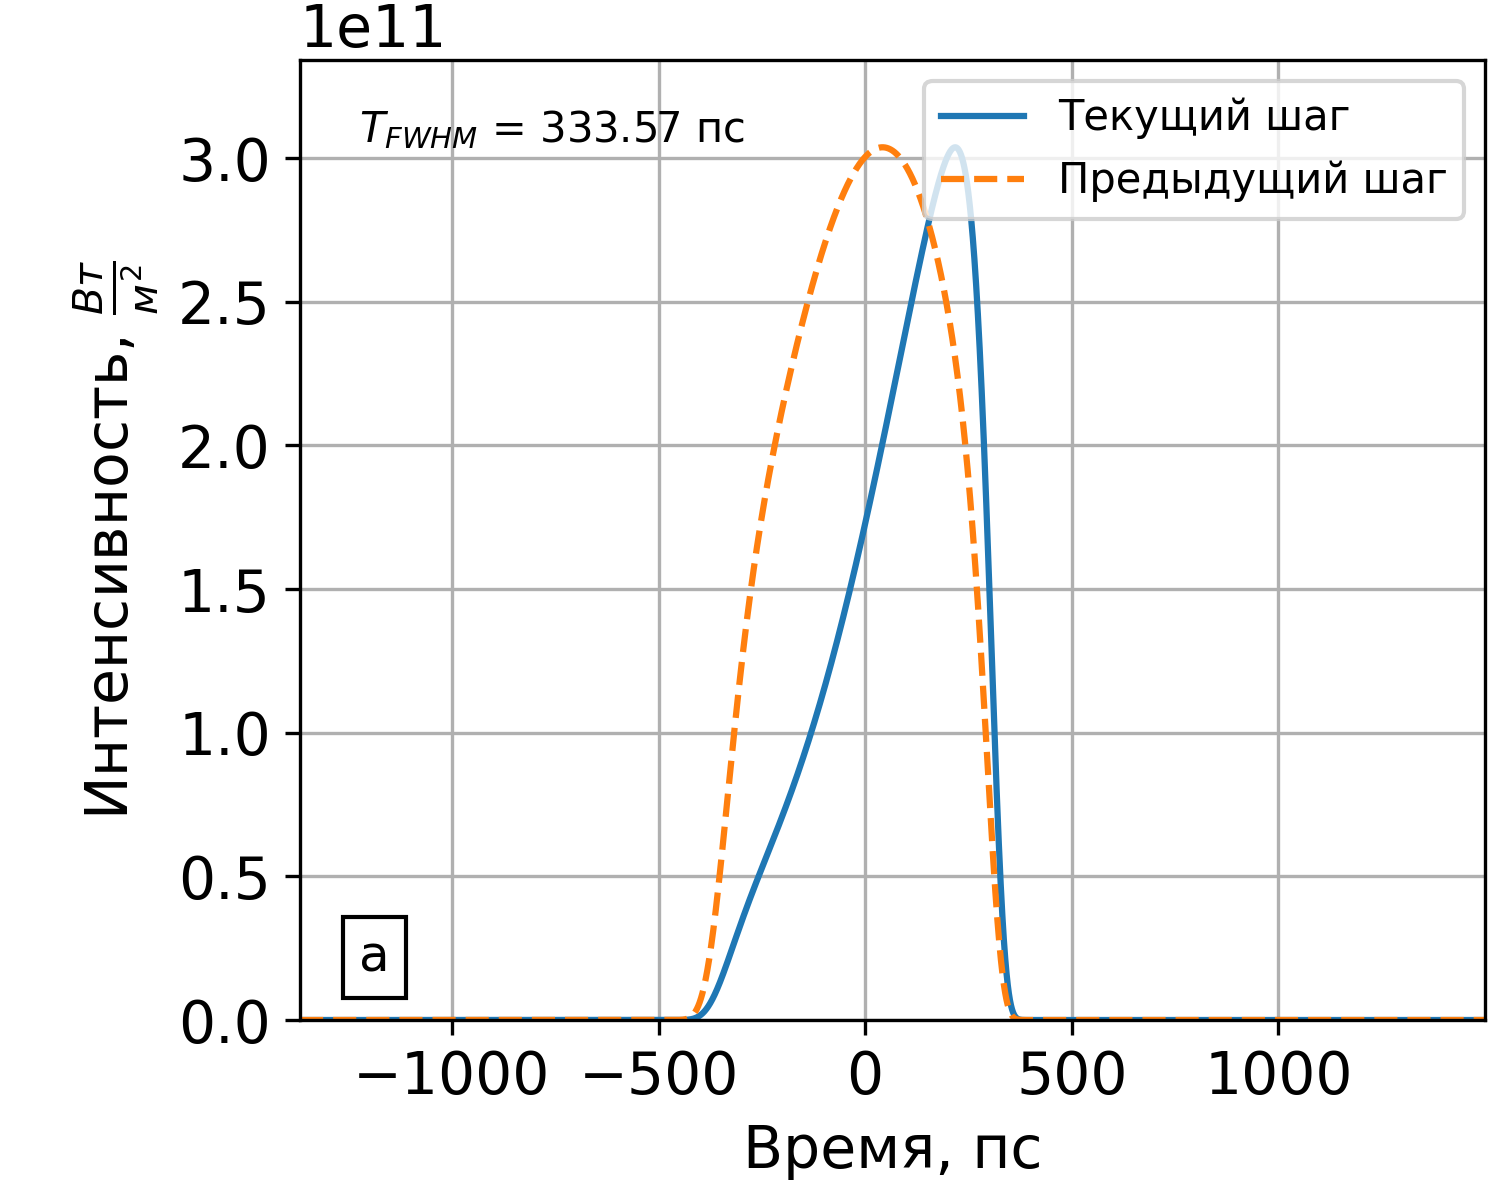
\includegraphics[width=\linewidth]{Images/Gauss Pulse/Импульс и спектр/!8. Yb3+ 6_125, 0.9m_pusle}
  \end{minipage}% <- % убирает хвостовой пробел / перевод строки
  \begin{minipage}[b]{0.5\textwidth}
    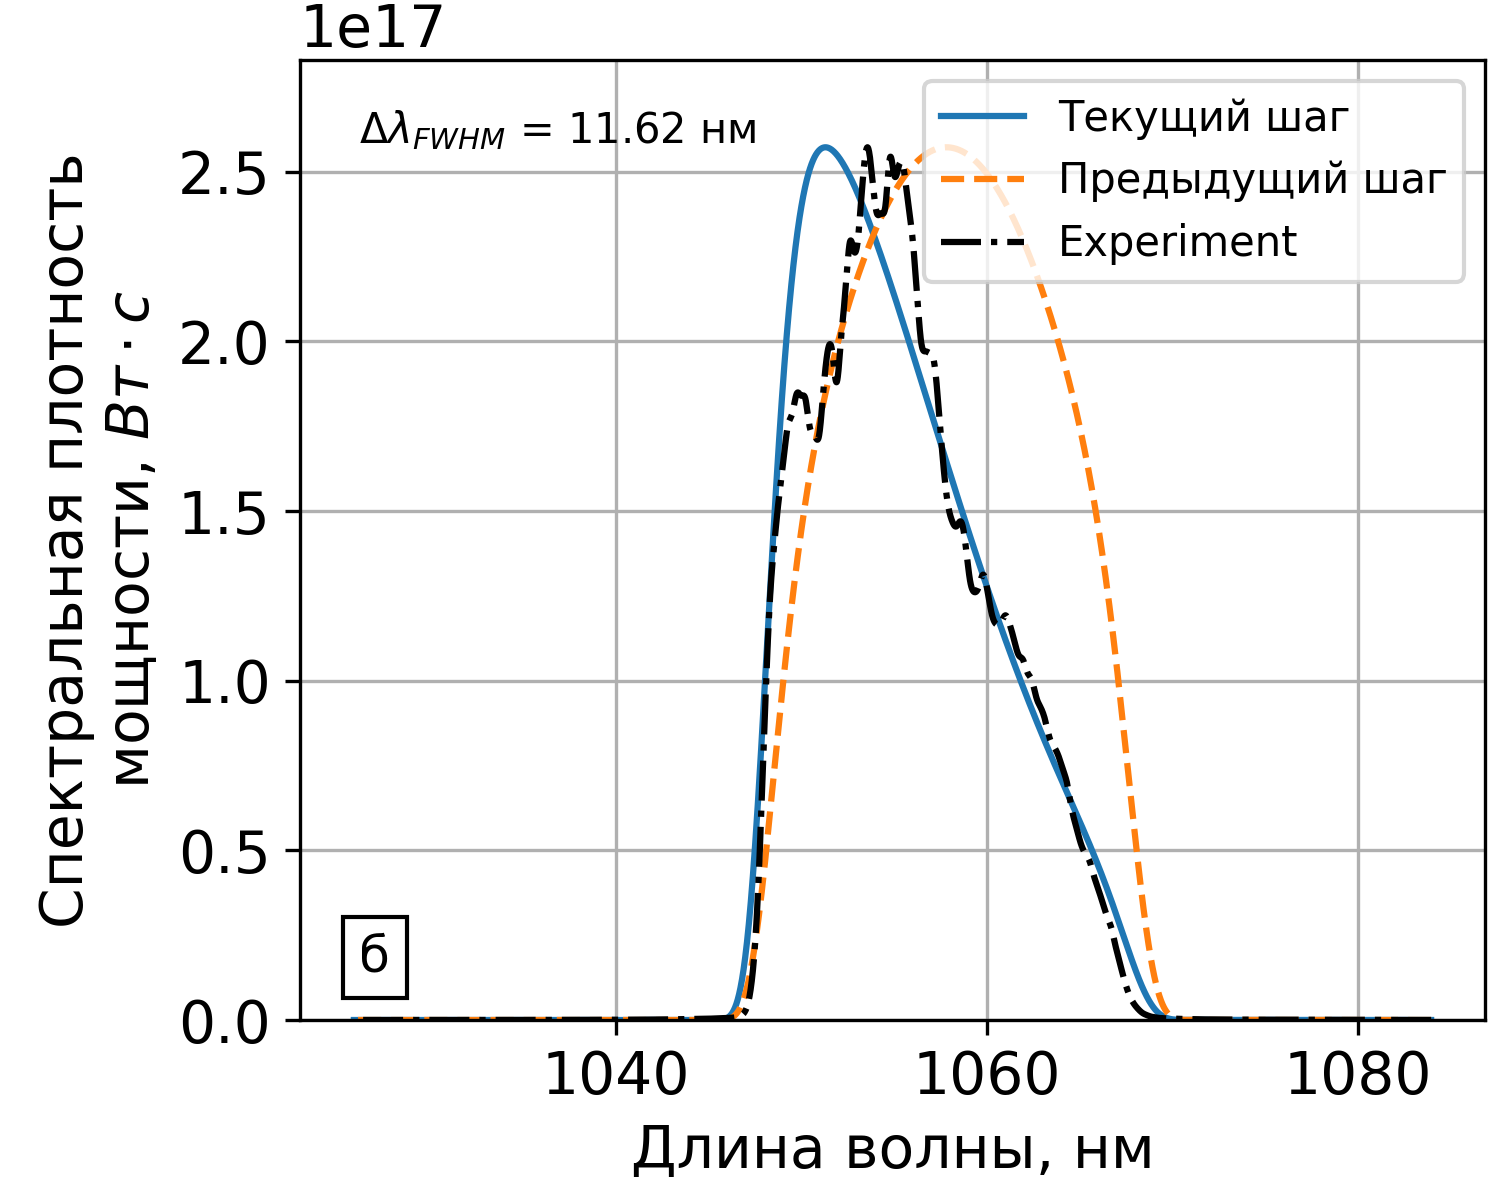
\includegraphics[width=\linewidth]{Images/Gauss Pulse/Импульс и спектр/!8. Yb3+ 6_125, 0.9m_spectrum}
  \end{minipage}

  \vspace{}

  \begin{minipage}[b]{0.5\textwidth}
    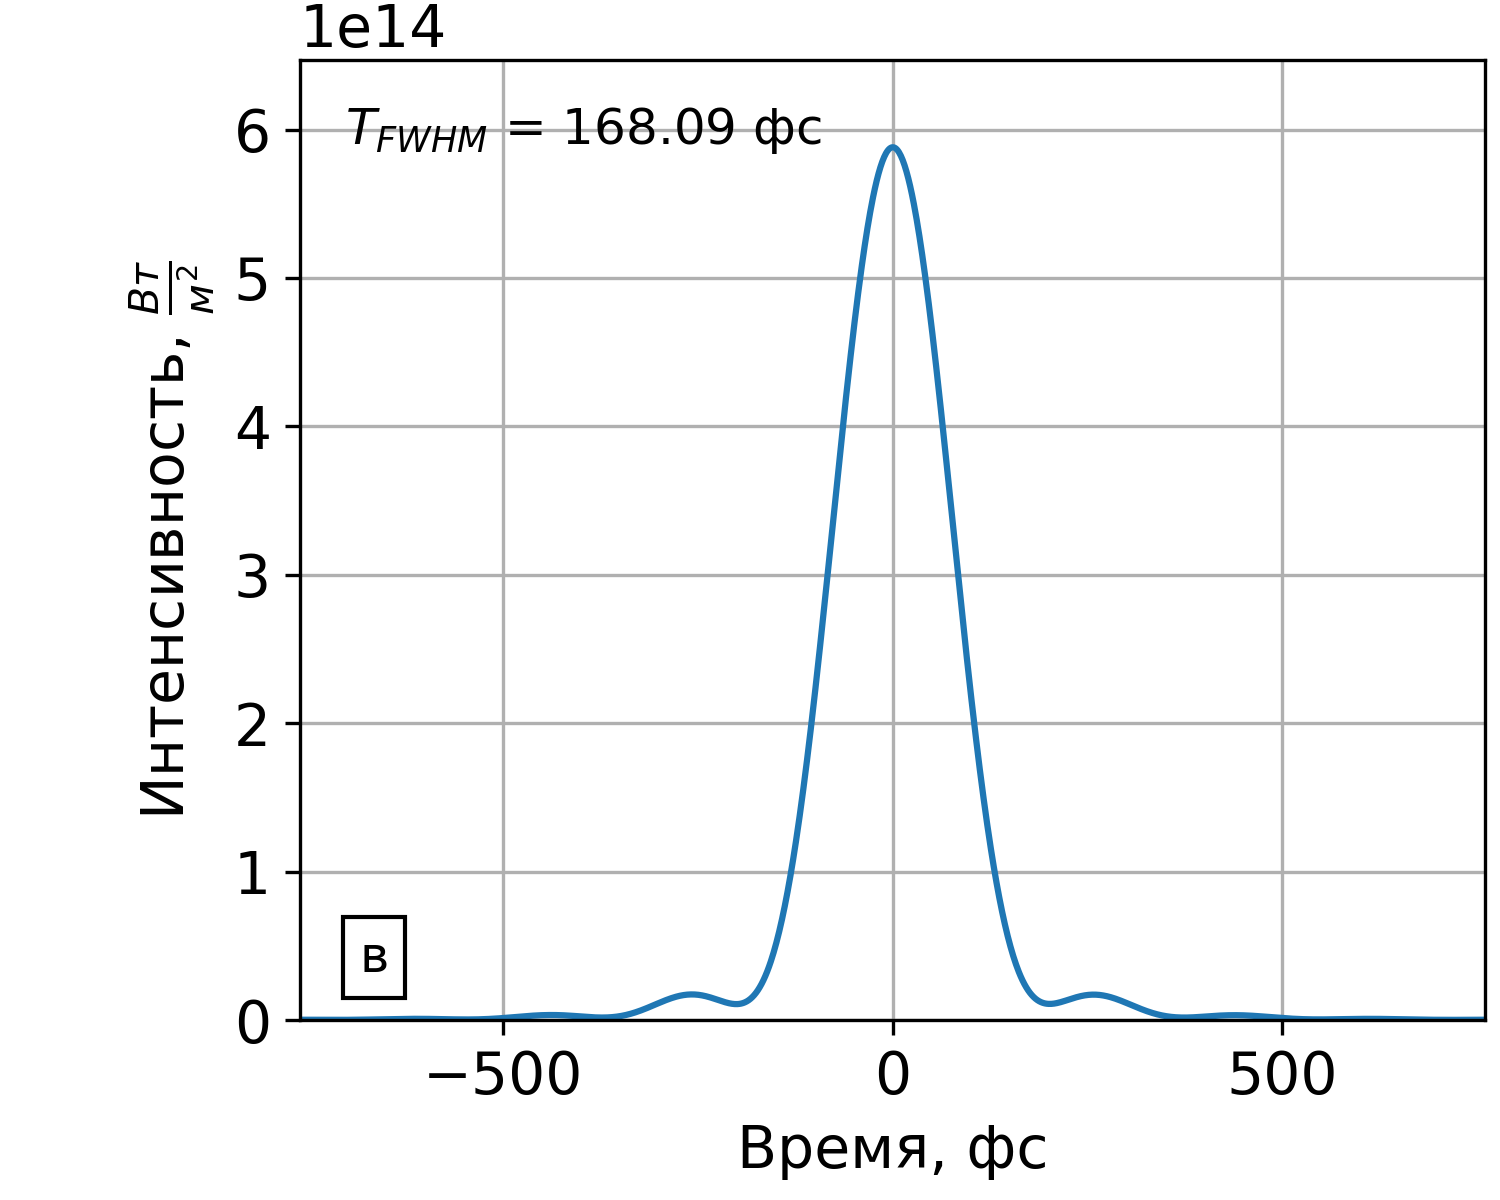
\includegraphics[width=\linewidth]{Images/Gauss Pulse/После компрессора/8 элемент gamma=49.49162 l_g=0.36725 сжатие}
  \end{minipage}% <- % убирает хвостовой пробел / перевод строки
  \begin{minipage}[b]{0.5\textwidth}
    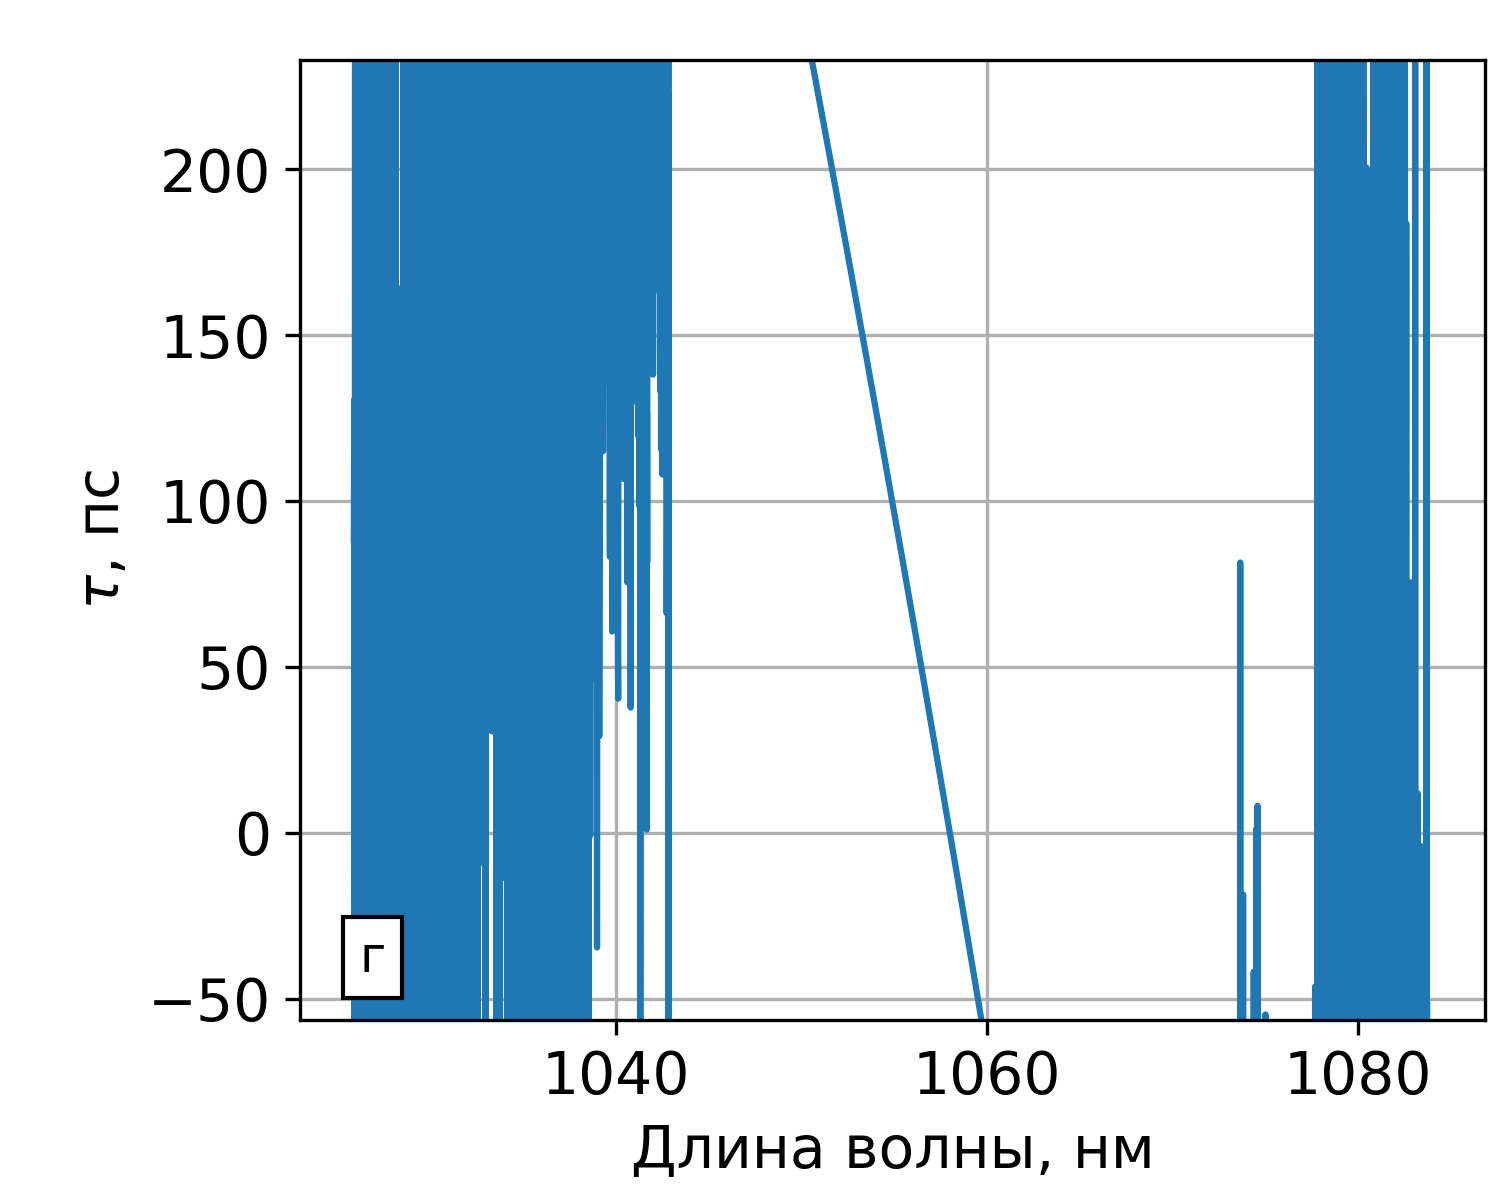
\includegraphics[width=\linewidth]{Images/Gauss Pulse/Импульс и спектр/!8. Yb3+ 6_125, 0.9m_time_delay}
  \end{minipage}

  \caption{Гауссов а) импульс, б) его спектр г) и групповая задержка после первого иттербиевого волокна (номер 5 на
  рисунке 2) с реальным профилем усиления. Приведён график г) импульса, сжатого в решёточном компрессоре}
  \label{fig:both}
\end{figure}

На рисунке 8 приведены графики импульса (рисунок 8а) после второго каскада усиления (номер 7 на рисунке 2). Усиление
делает спектр (рисунок 8б) ещё более несимметричным. Задний фронт импульса становится крутым, тогда как
передний пологим. Спектр импульса становится уже, поэтому длительность, получаемая после компрессора, увеличивается.
При этом энергия импульса становится примерно 40 нДж, что даёт $B$-интеграл в следующем элементе больше 7, поэтому фазовая
модуляция начинает играть большую роль в изменении фазы. Подробнее это рассмотрено ниже.

\begin{figure}[h!]
  \centering
  \begin{minipage}[b]{0.5\textwidth}
    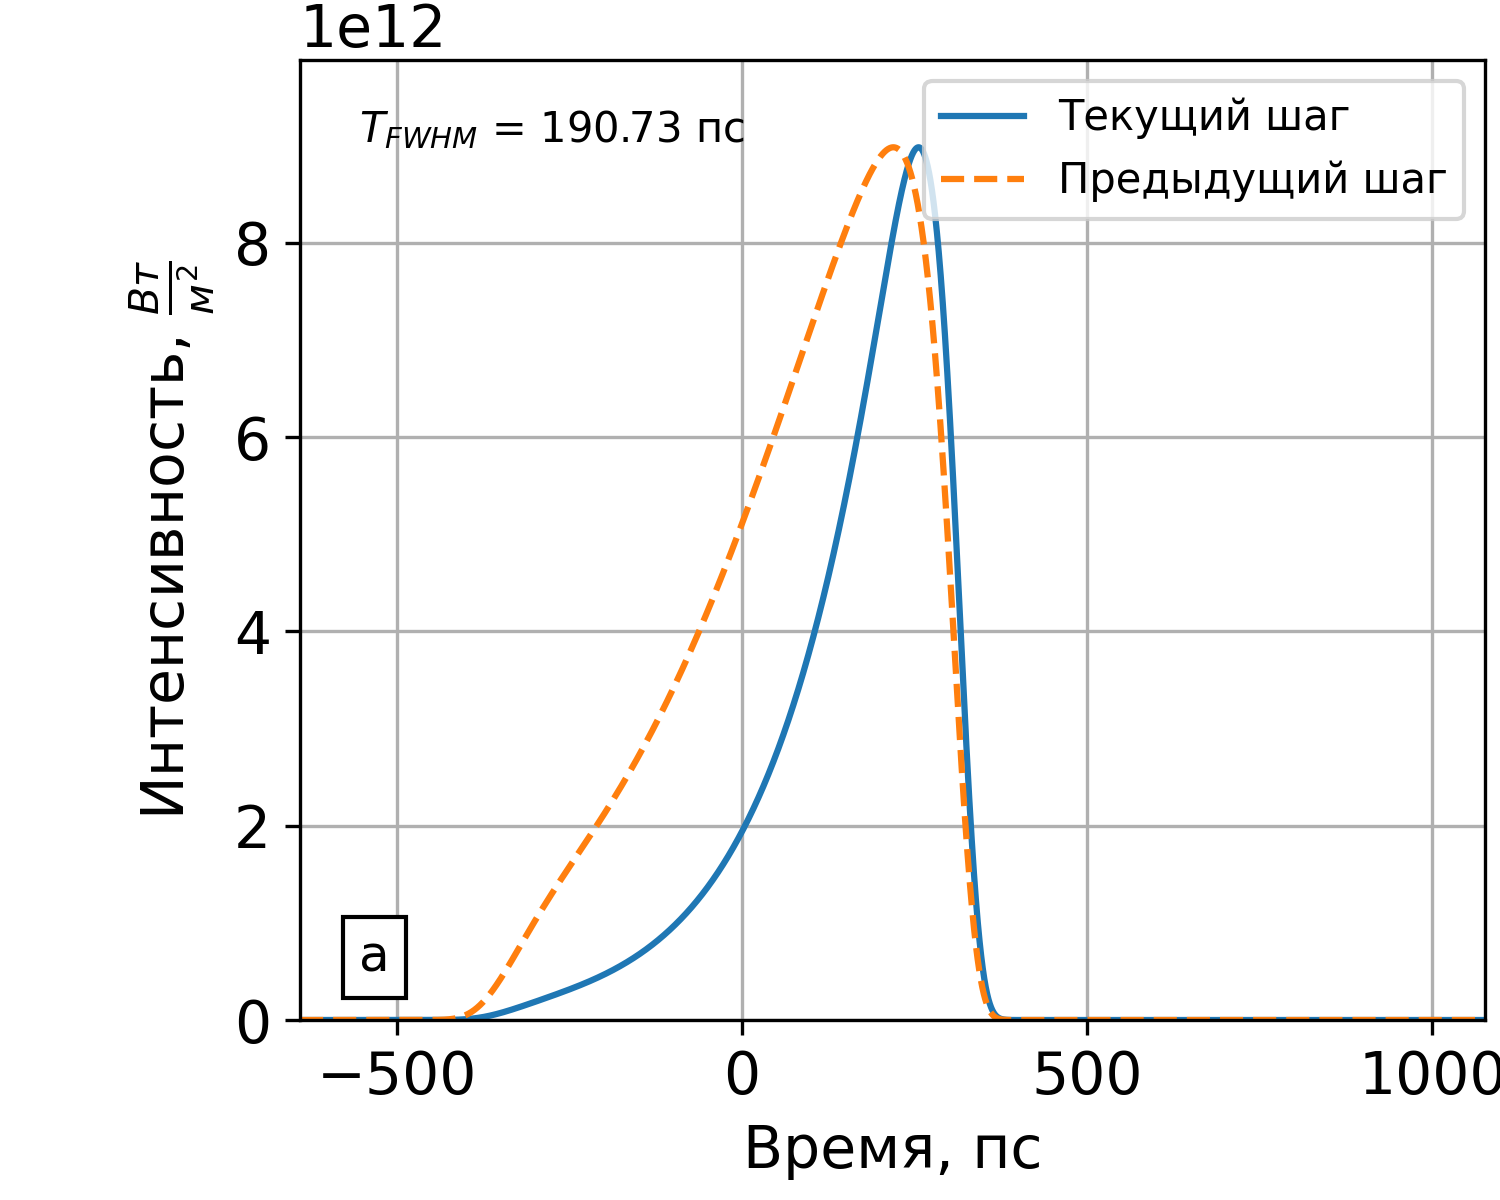
\includegraphics[width=\linewidth]{Images/Gauss Pulse/Импульс и спектр/!14. Yb3+ 6_125, 0.8m_pusle}
  \end{minipage}% <- % убирает хвостовой пробел / перевод строки
  \begin{minipage}[b]{0.5\textwidth}
    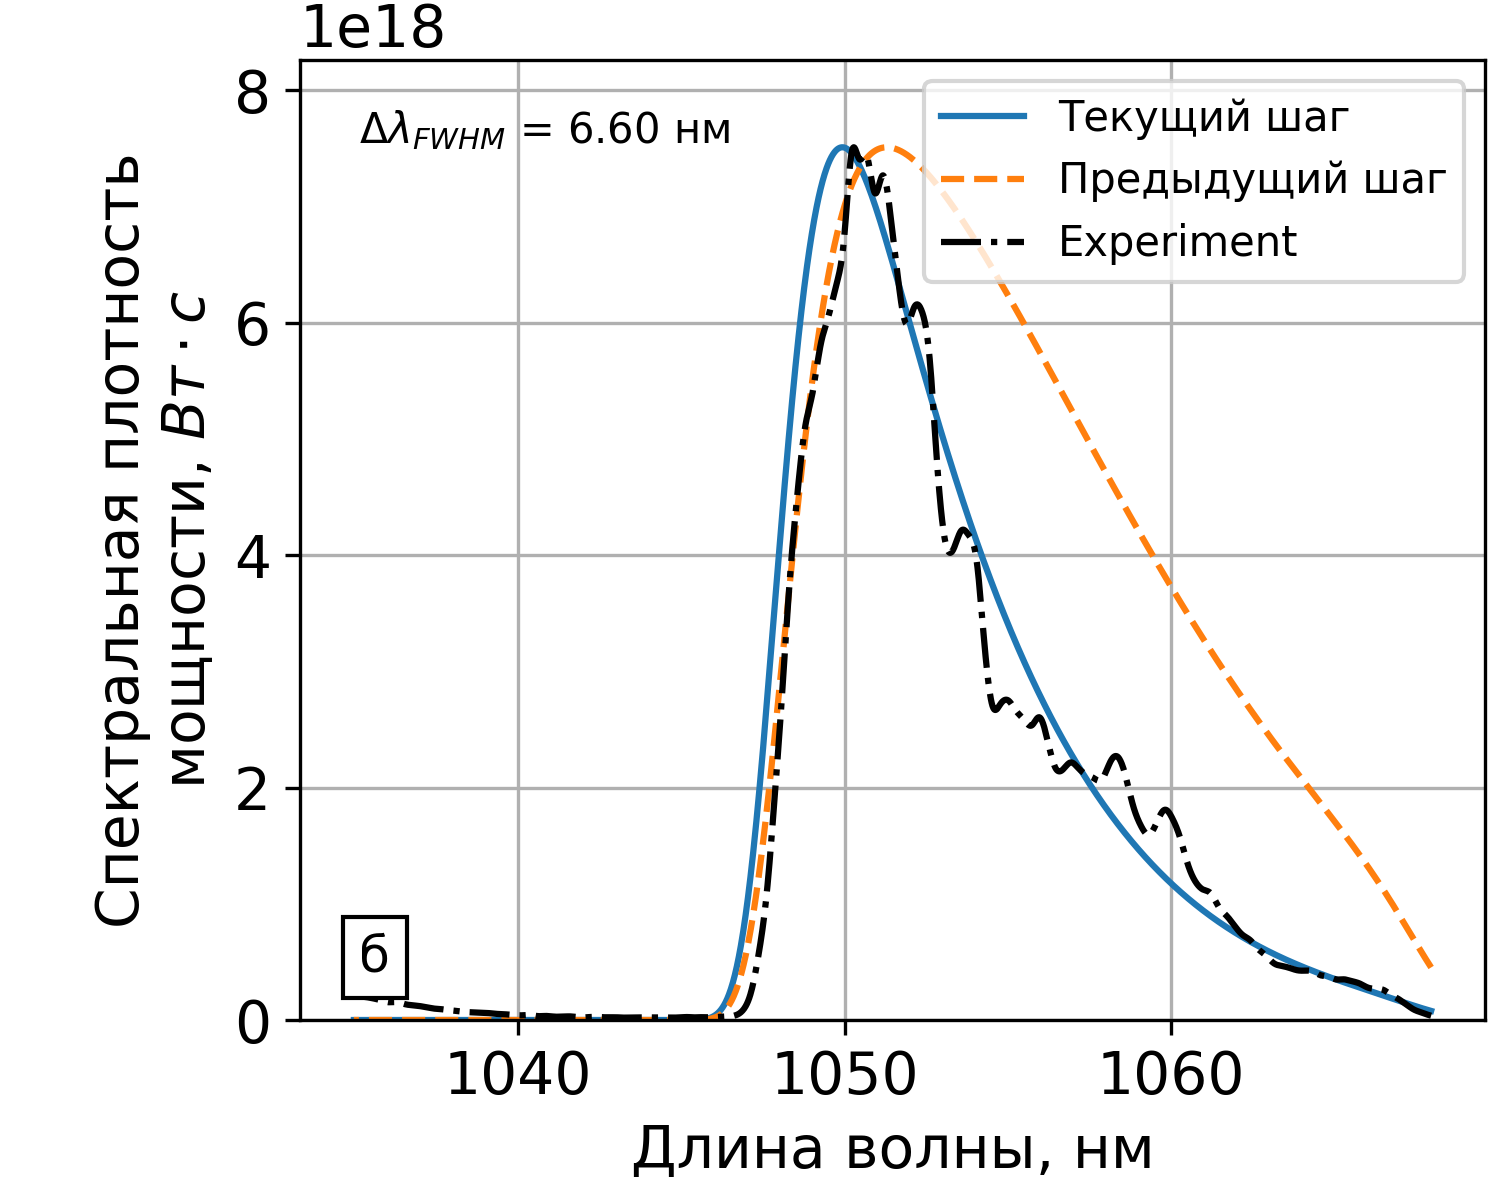
\includegraphics[width=\linewidth]{Images/Gauss Pulse/Импульс и спектр/!14. Yb3+ 6_125, 0.8m_spectrum}
  \end{minipage}

  \vspace{}

  \begin{minipage}[b]{0.5\textwidth}
    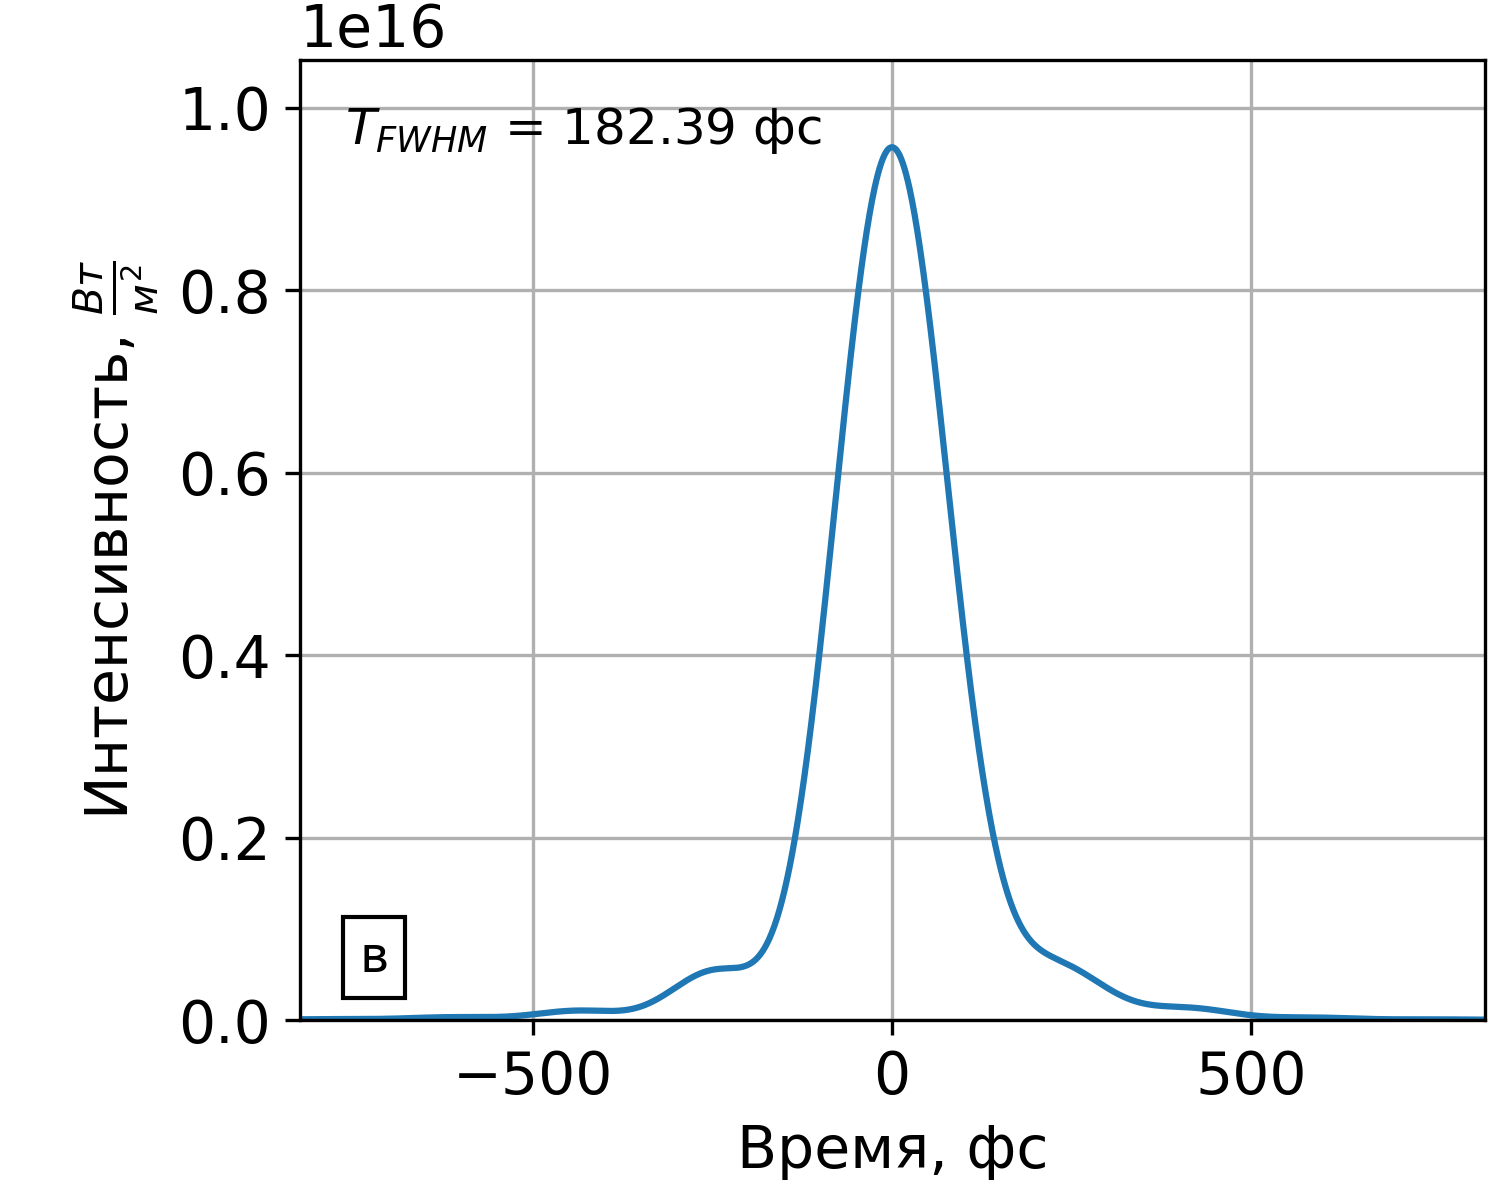
\includegraphics[width=\linewidth]{Images/Gauss Pulse/После компрессора/14 элемент gamma=49.71717 l_g=0.37698 сжатие}
  \end{minipage}% <- % убирает хвостовой пробел / перевод строки
  \begin{minipage}[b]{0.5\textwidth}
    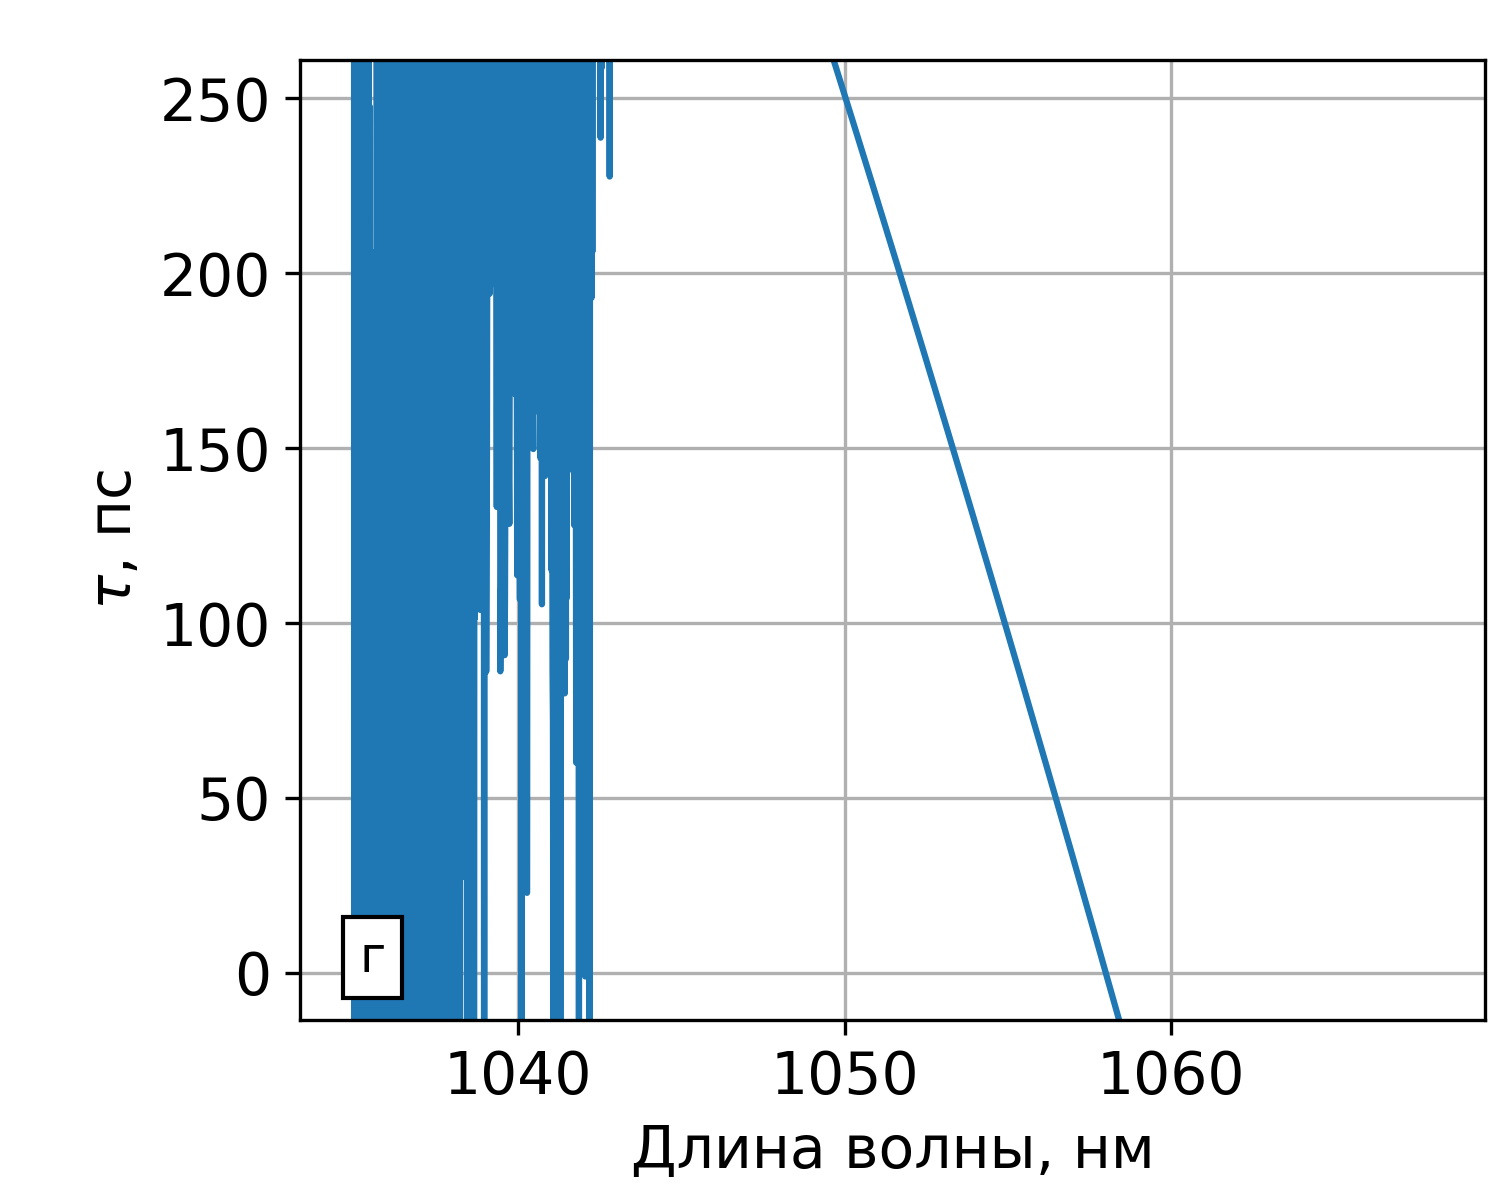
\includegraphics[width=\linewidth]{Images/Gauss Pulse/Импульс и спектр/!14. Yb3+ 6_125, 0.8m_time_delay}
  \end{minipage}

  \caption{Гауссов а) импульс, б) его спектр г) и групповая задержка после второго иттербиевого волокна (номер 7 на
  рисунке 2) с реальным профилем усиления. Приведён график г) импульса, сжатого в решёточном компрессоре}
  \label{fig:both}
\end{figure}

На рисунке 9 приведено состояние импульса (рисунок 9а) после последнего каскада и импульс, сжатый компрессором (рисунок 9в),
то есть тот, который получается на выходе из оптической установки. После последнего каскада усиления энергия импульса чуть
больше 1 мкДж, что при частоте повторения 1 МГц даёт среднюю мощность чуть больше 1 Вт. По сравнению со вторым каскадом
форма спектра (рисунок 9б) изменяется уже не очень сильно. При этом на сжатом импульсе начинают появляться осцилляции.

Чтобы понять, что именно влияет на ухудшение способности к сжатию импульса, проанализируем спектральную фазу импульса.
Для получения коэффициентов её разложения в ряд использовалась аппроксимация полиномом 5 порядка:

\begin{equation}
    \varphi(\omega) \approx \sum_{n=0}^5 \frac{\beta_n}{n!} (\omega - \omega_0)^n
\end{equation}

На рисунке 10 представлены графики, которые отражают вклад каждого из элементов в $\beta_2$.
Как можем видеть, все волокна изменяют $\beta_2$ в положительную сторону, чего и следовало ожидать для этой длины волны.
Однако второй порядок точно скомпенсирован решёточным компрессором, поэтому $\beta_2$ не влияет на способность импульса
к сжатию.

\begin{figure}[h!]
  \centering
  \begin{minipage}[b]{0.5\textwidth}
    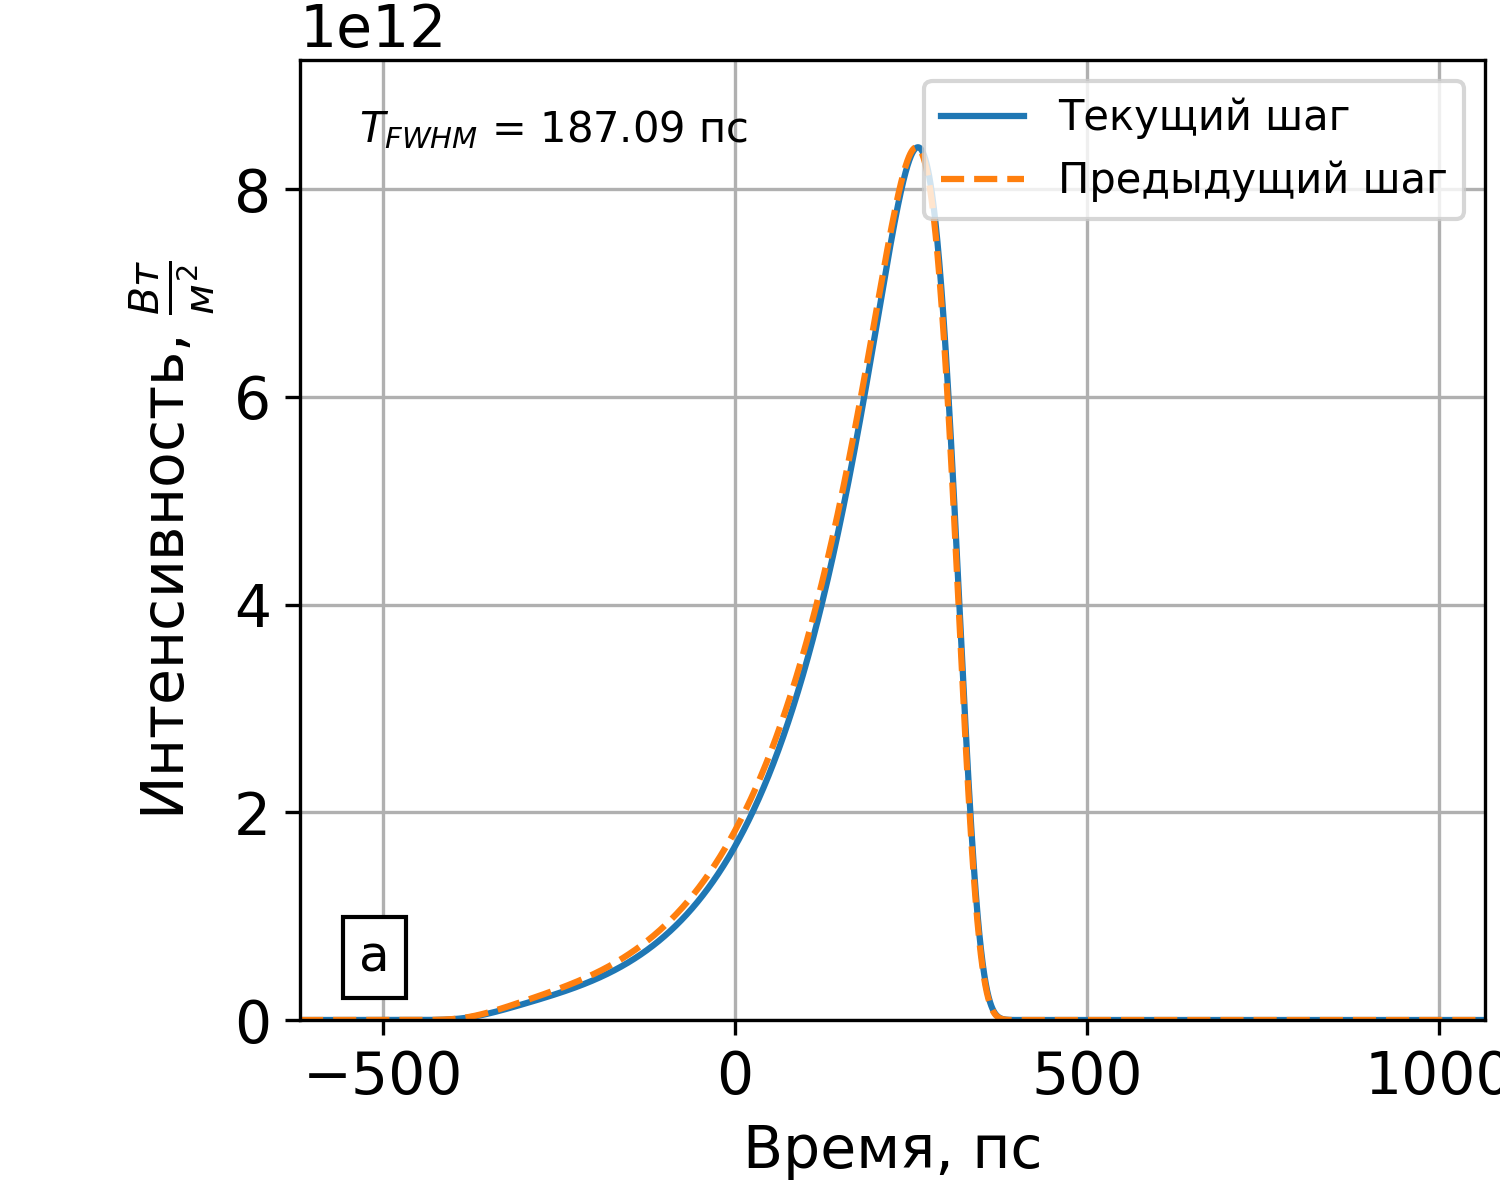
\includegraphics[width=\linewidth]{Images/Gauss Pulse/Импульс и спектр/!23. Fiber_pusle}
  \end{minipage}% <- % убирает хвостовой пробел / перевод строки
  \begin{minipage}[b]{0.5\textwidth}
    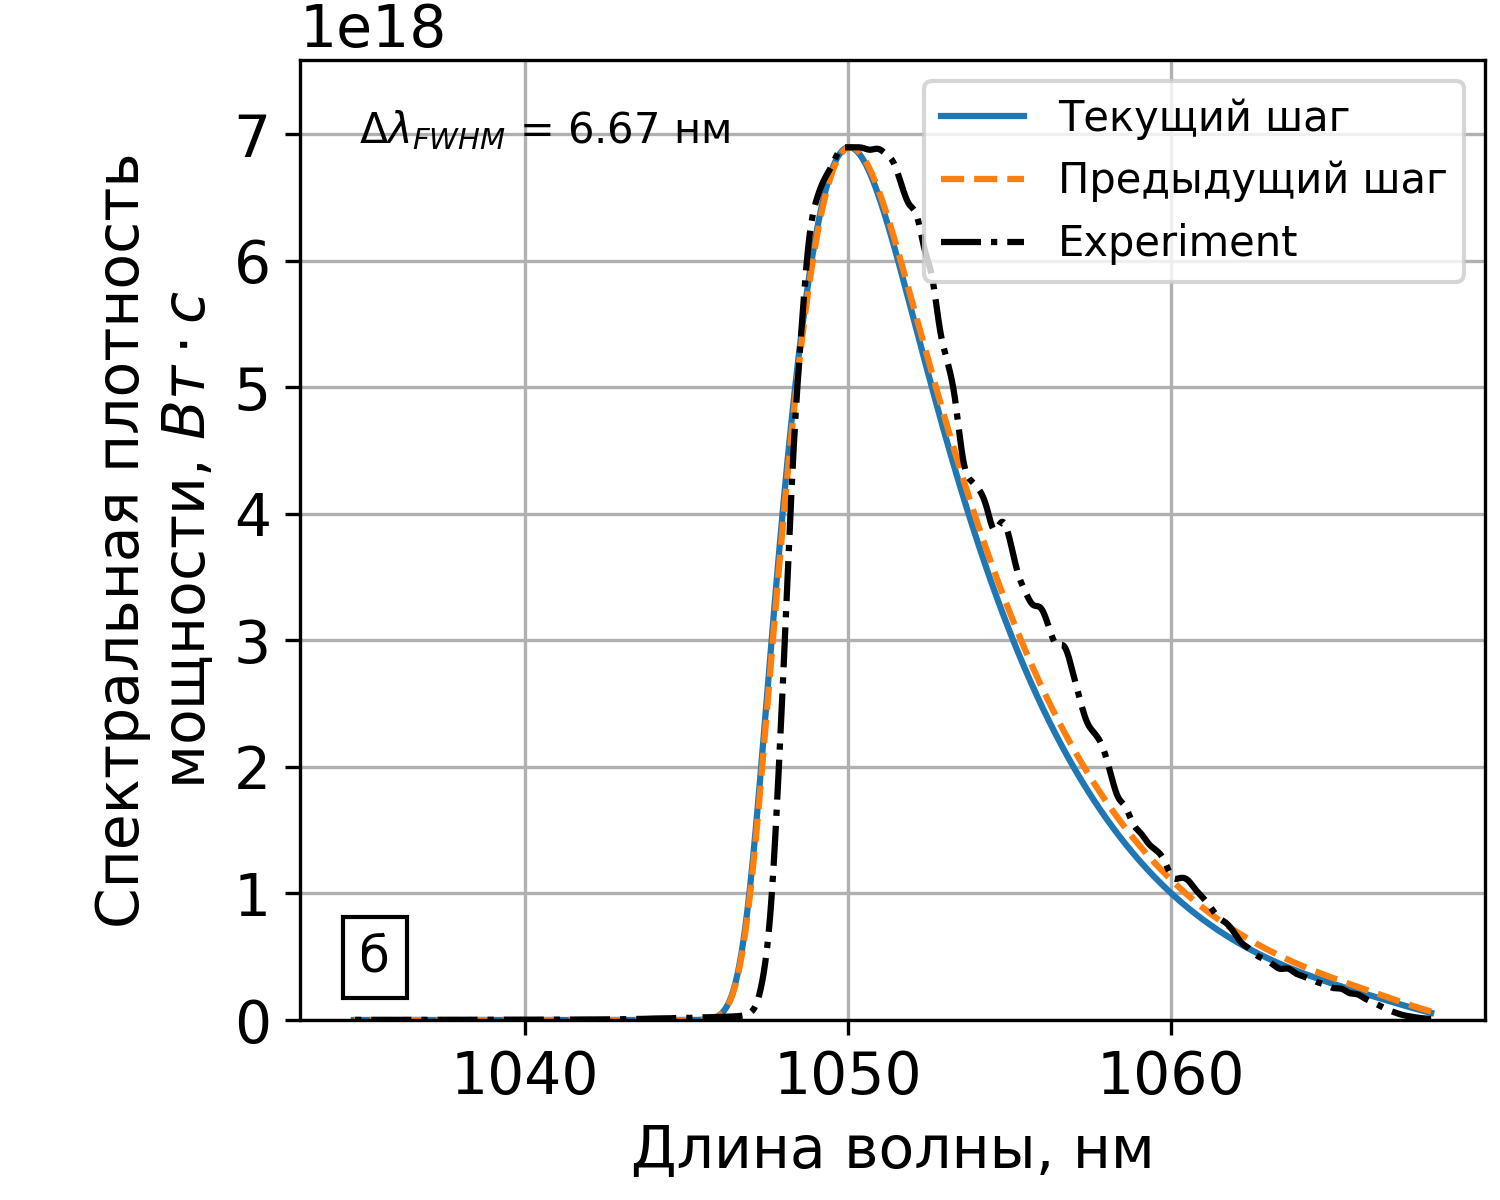
\includegraphics[width=\linewidth]{Images/Gauss Pulse/Импульс и спектр/!23. Fiber_spectrum}
  \end{minipage}

  \vspace{}

  \begin{minipage}[b]{0.5\textwidth}
    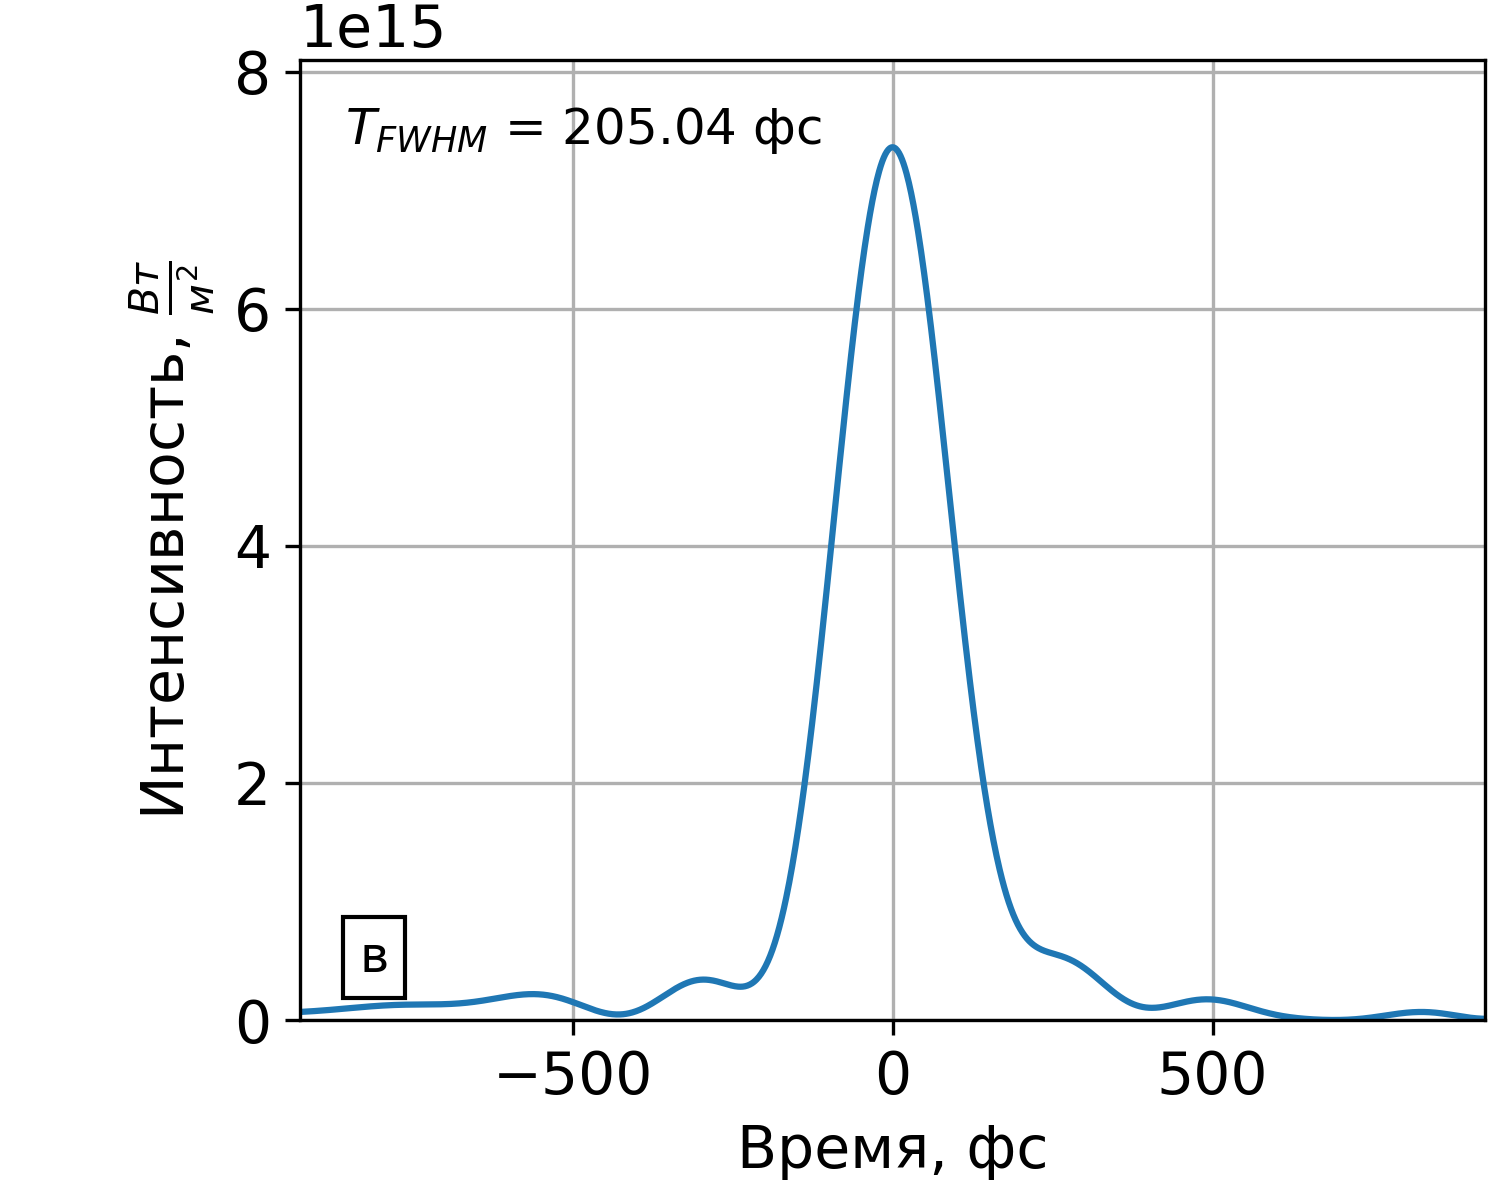
\includegraphics[width=\linewidth]{Images/Gauss Pulse/После компрессора/23 элемент gamma=51.86558 l_g=0.45239 сжатие}
  \end{minipage}% <- % убирает хвостовой пробел / перевод строки
  \begin{minipage}[b]{0.5\textwidth}
    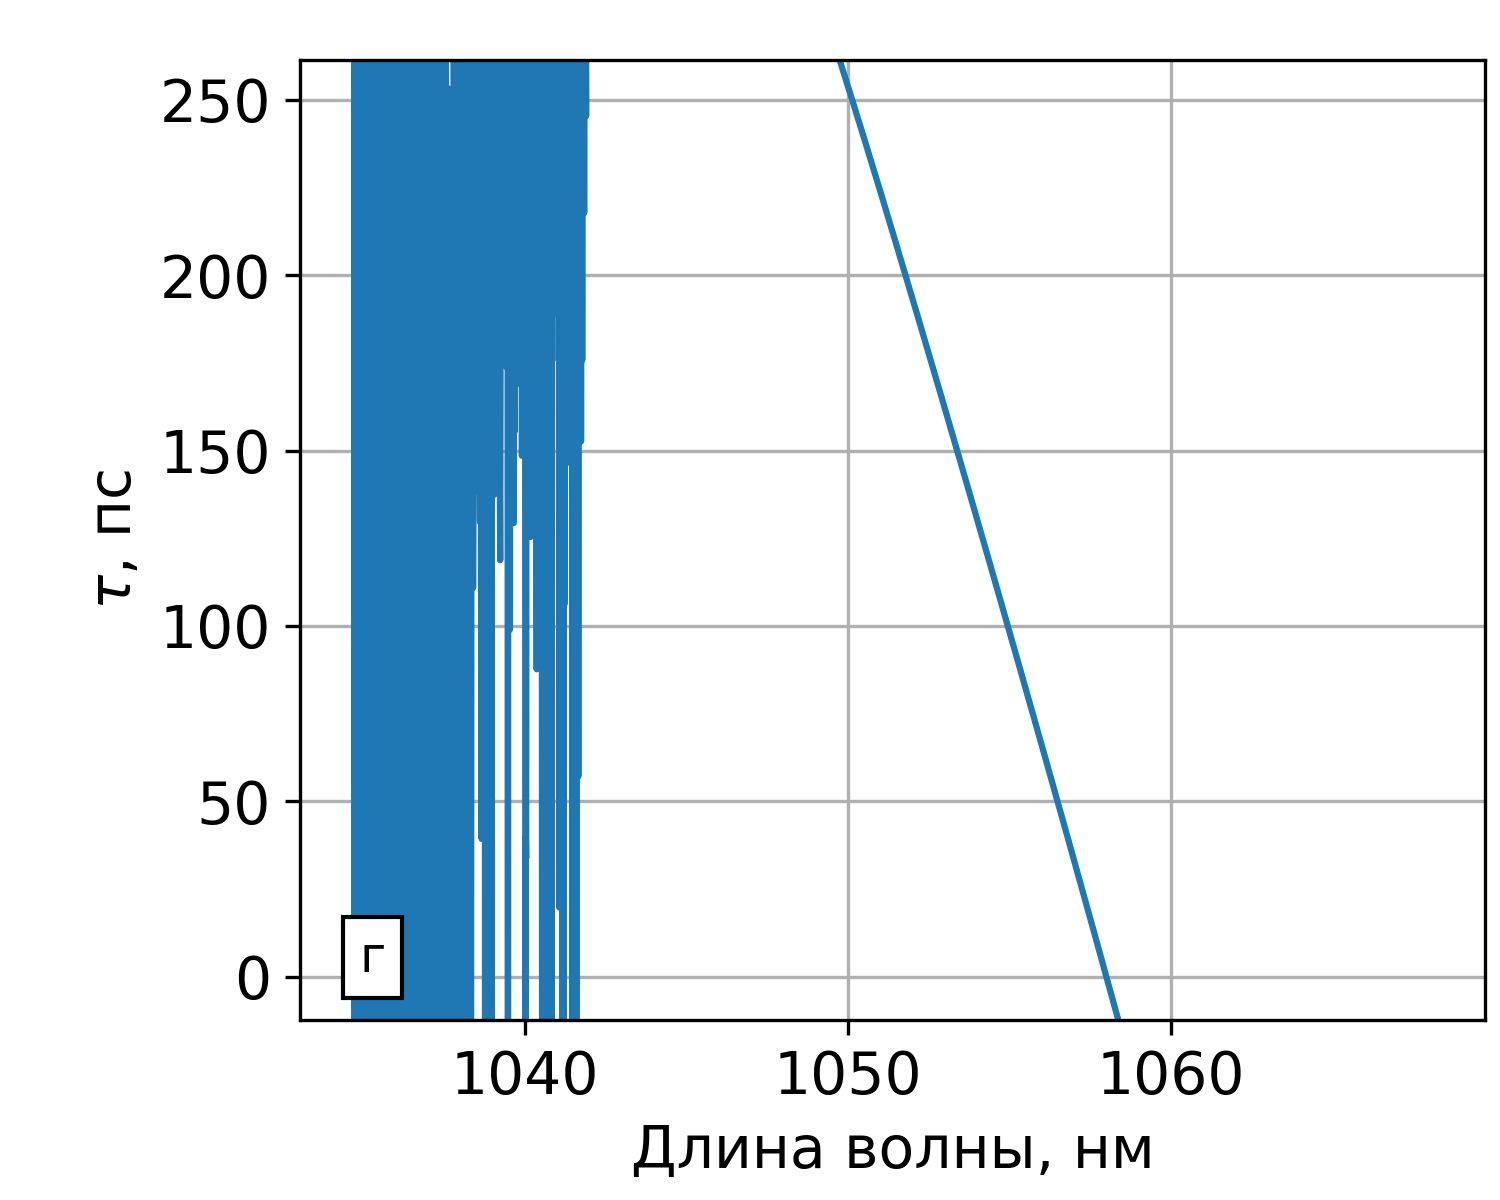
\includegraphics[width=\linewidth]{Images/Gauss Pulse/Импульс и спектр/!23. Fiber_time_delay}
  \end{minipage}

  \caption{Гауссов а) импульс, б) его спектр г) и групповая задержка после третьего иттербиевого волокна (номер 10 на
  рисунке 2) с реальным профилем усиления. Приведён график г) импульса, сжатого в решёточном компрессоре}
  \label{fig:both}
\end{figure}

\begin{figure}[h!]
    \centering
    \begin{minipage}[b]{0.5\textwidth}
        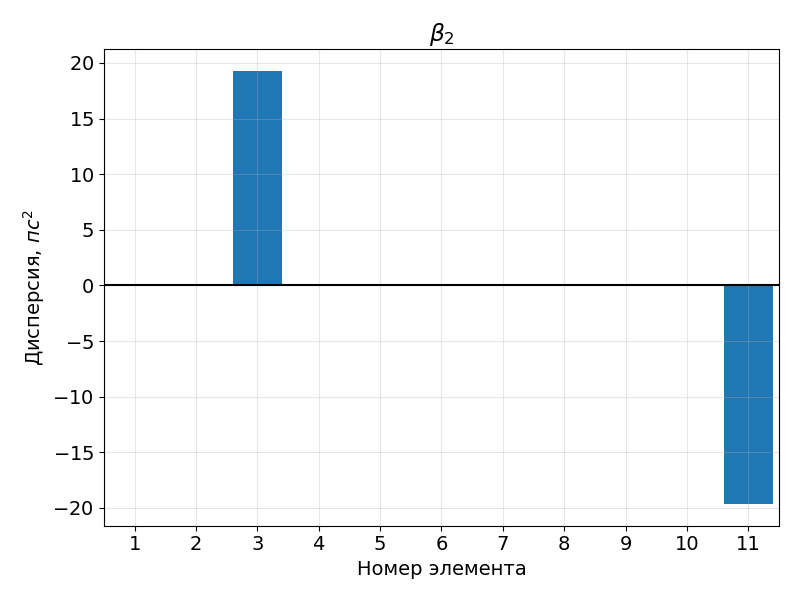
\includegraphics[width=\linewidth]{Images/Gauss Pulse/Беты/beta_2_full}
    \end{minipage}% <- % убирает хвостовой пробел / перевод строки
    \begin{minipage}[b]{0.5\textwidth}
        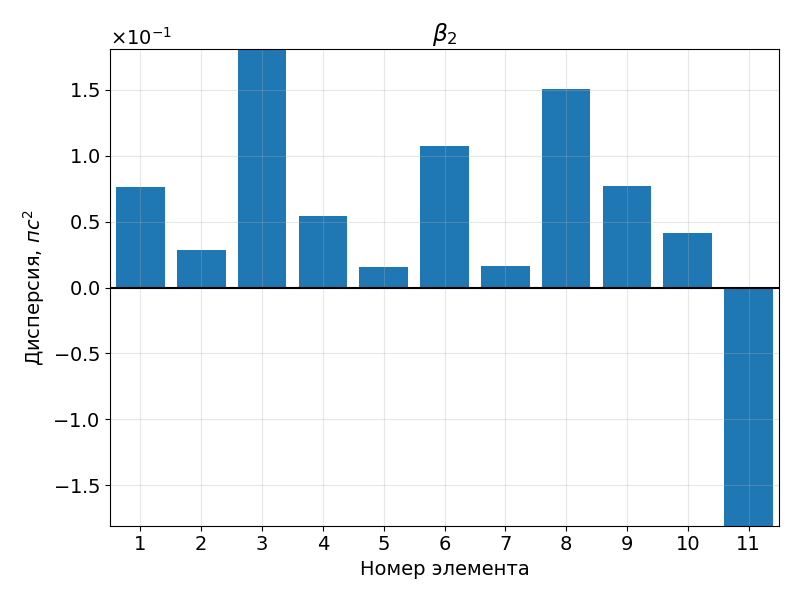
\includegraphics[width=\linewidth]{Images/Gauss Pulse/Беты/beta_2_cut}
    \end{minipage}

    \caption{Коэффициенты $\beta_2$, рассчитанные с помощью аппроксимации спектальной фазы полиномом,
     в двух масштабах (слева общий масштаб, справа увеличенный)}
    \label{fig:both}
\end{figure}

Для $\beta_3$, графики которого представлены на рисунке 11, картина получается более интересной.
Обратим внимание, что после 7 элемента — второго каскада усиления — видно отчётливое увеличение вклада волокна.
Получается, что фазовая самомодуляция довольно сильно изменяет набег фазы в 8 элементе.

\begin{figure}[h!]
    \centering
    \begin{minipage}[b]{0.5\textwidth}
        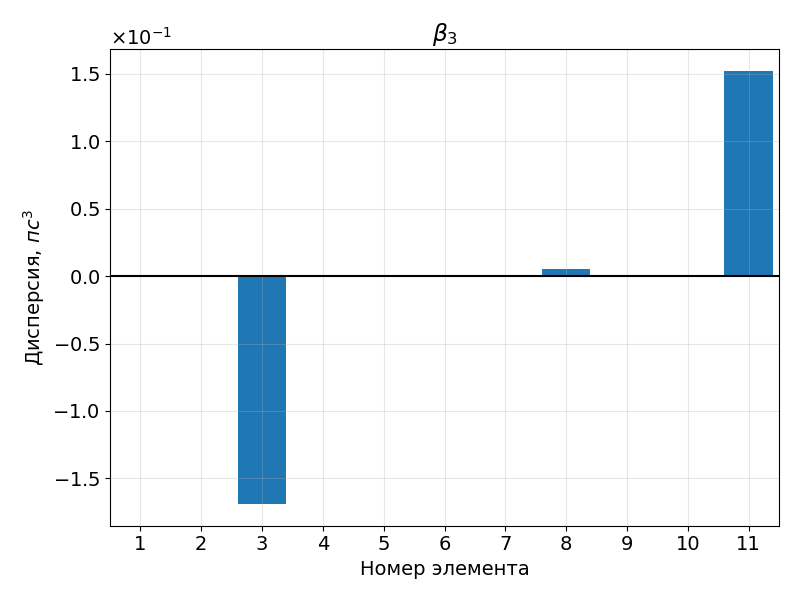
\includegraphics[width=\linewidth]{Images/Gauss Pulse/Беты/beta_3_full}
    \end{minipage}% <- % убирает хвостовой пробел / перевод строки
    \begin{minipage}[b]{0.5\textwidth}
        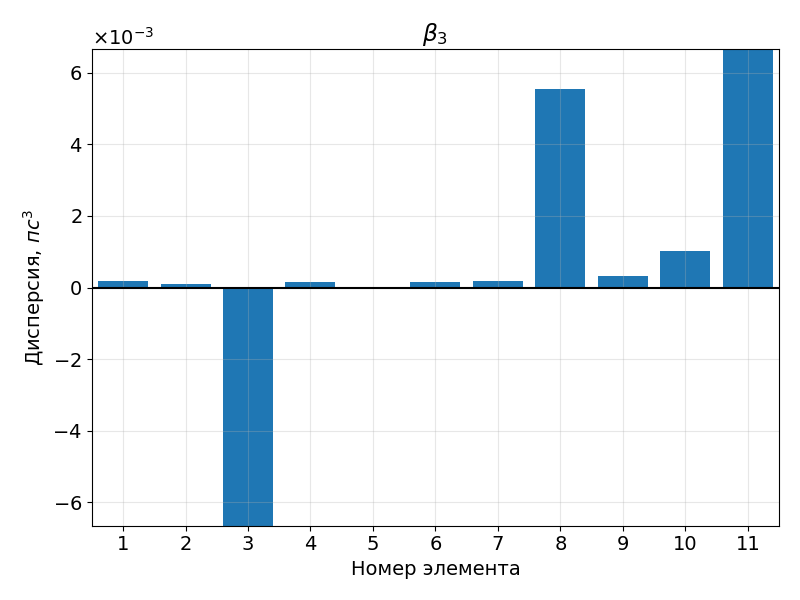
\includegraphics[width=\linewidth]{Images/Gauss Pulse/Беты/beta_3_cut}
    \end{minipage}

    \caption{Коэффициенты $\beta_3$, рассчитанные с помощью аппроксимации спектальной фазы полиномом,
     в двух масштабах (слева общий масштаб, справа увеличенный)}
    \label{fig:both}
\end{figure}

Для четвёртого порядка, представленного на рисунке 12, ситуация повторяется: фазовая самомодуляция после второго каскада
усиления вызывает сильный набег фазы, который уже сопоставим с влияниями брэгговской решётки и компрессора. Поэтому при
сжатии он не компенсируется, что вызывает пост- и предымпульсы. Обратим внимание на разницу модулирования фазы между
8 и 9 элементом. 8 элемент — волокно с диаметром 6 мкм, а 9 элемент — 25 мкм. Фазовая самомодуляция определяется интенсивностью
поля и параметром $\gamma(\omega)$, в знаменателе которого стоит эффективная площадь моды. При её увеличении вклад
фазовой самомодуляции заметно уменьшается, что подтверждает предположении о причинах ухудшения способности к сжатию
импульса.

\begin{figure}[h!]
    \centering
    \begin{minipage}[b]{0.5\textwidth}
        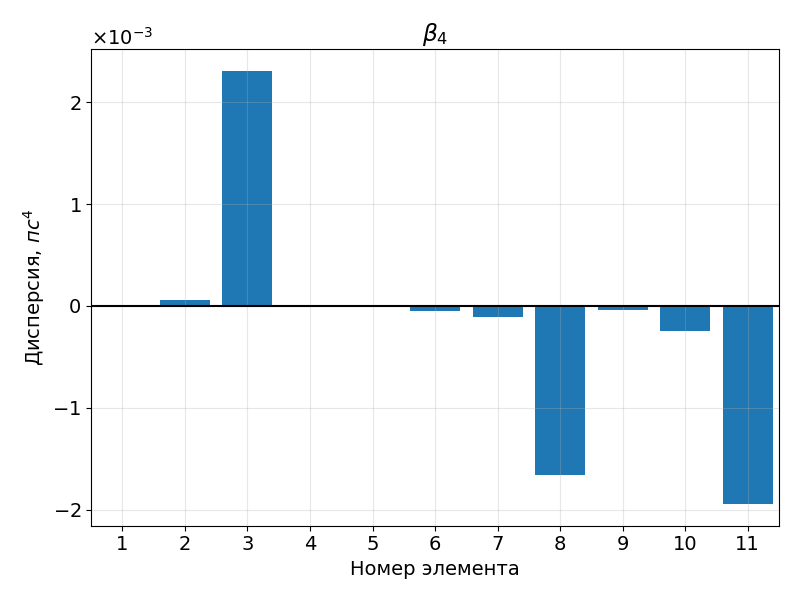
\includegraphics[width=\linewidth]{Images/Gauss Pulse/Беты/beta_4_full}
    \end{minipage}% <- % убирает хвостовой пробел / перевод строки
    \begin{minipage}[b]{0.5\textwidth}
        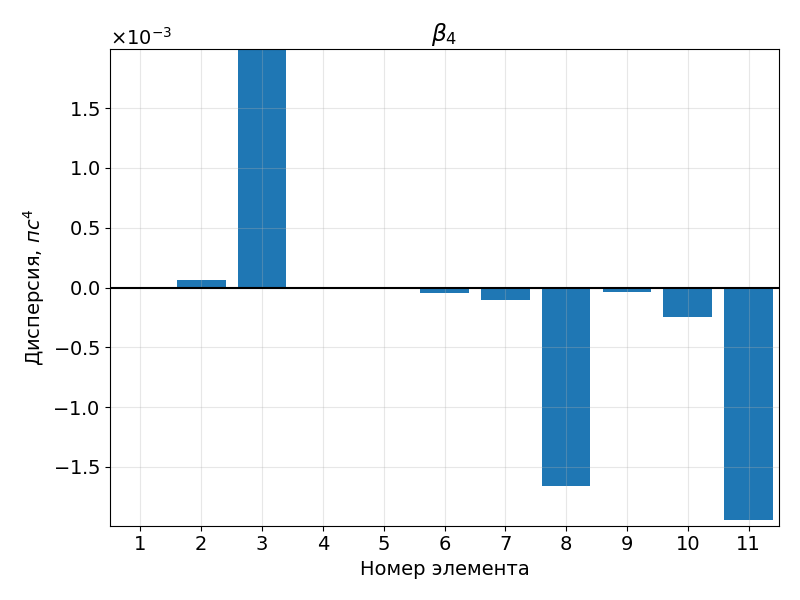
\includegraphics[width=\linewidth]{Images/Gauss Pulse/Беты/beta_4_cut}
    \end{minipage}

    \caption{Коэффициенты $\beta_4$, рассчитанные с помощью аппроксимации спектальной фазы полиномом,
     в двух масштабах (слева общий масштаб, справа увеличенный)}
    \label{fig:both}
\end{figure}

Предположения подтверждает и расчёт B-интегралов, которые отражают максимальное изменение фазы:

\begin{equation}
    \varphi_{max}(\omega, z) = \int_0^L \gamma(\omega) P_0(z)\,dz,
\end{equation}

где $P_0(z)$ — пиковая мощность импульса. На рисунке 13 видно, что после второго каскада усиления (элемент 8) фазовая
самомодуляция вызывает набег больше, чем на 7 радиан, что и ухудшает способность импульса к сжатию.

\begin{figure}[h!]
    \centering
    \begin{minipage}[b]{0.5\textwidth}
        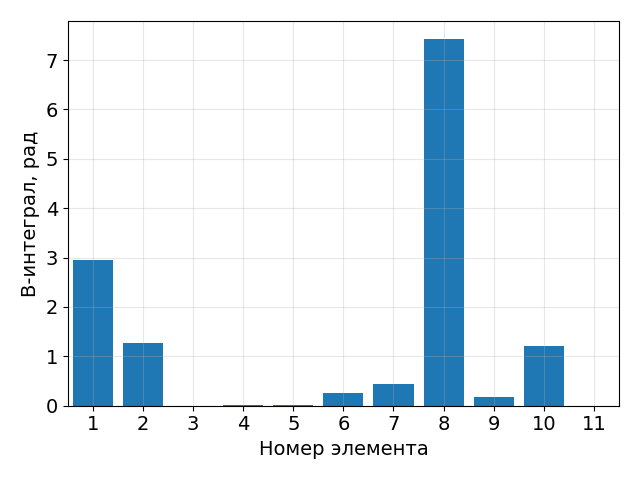
\includegraphics[width=\textwidth]{Images/Gauss Pulse/!B интегралы}
    \end{minipage}
    \caption{График $B$-интеграла на каждом элементе, изображённом в схеме установки на рисунке 2}
\end{figure}

\subsection{Моделирование гауссова импульса с параболическим спетром усиления}

Выше было отмечено, что спектр усиления $Yb^{3+}$ делает спектр несимметричным, что ухудшает качество импульса.
Чтобы посмотреть, как профиль усиления на это влияет, промоделируем параболический профиль, заданный формулой:

\begin{equation}
    g = \frac{g_0}{1 + \frac{W(z)}{W_s}} \Bigl( 1 + \Delta^2 \frac{\partial^2}{\partial \tau^2} \Bigr),
\end{equation}

где $g_0$ — коэффициент усиления, $W_s$ — энергия насыщения, $\Delta^{-1}$ — ширина спектра усиления,

\begin{equation}
    W(z) = \int_{t} |E|^2 \,d\tau,
\end{equation}

\begin{figure}[h!]
  \centering
  \begin{minipage}[b]{0.5\textwidth}
    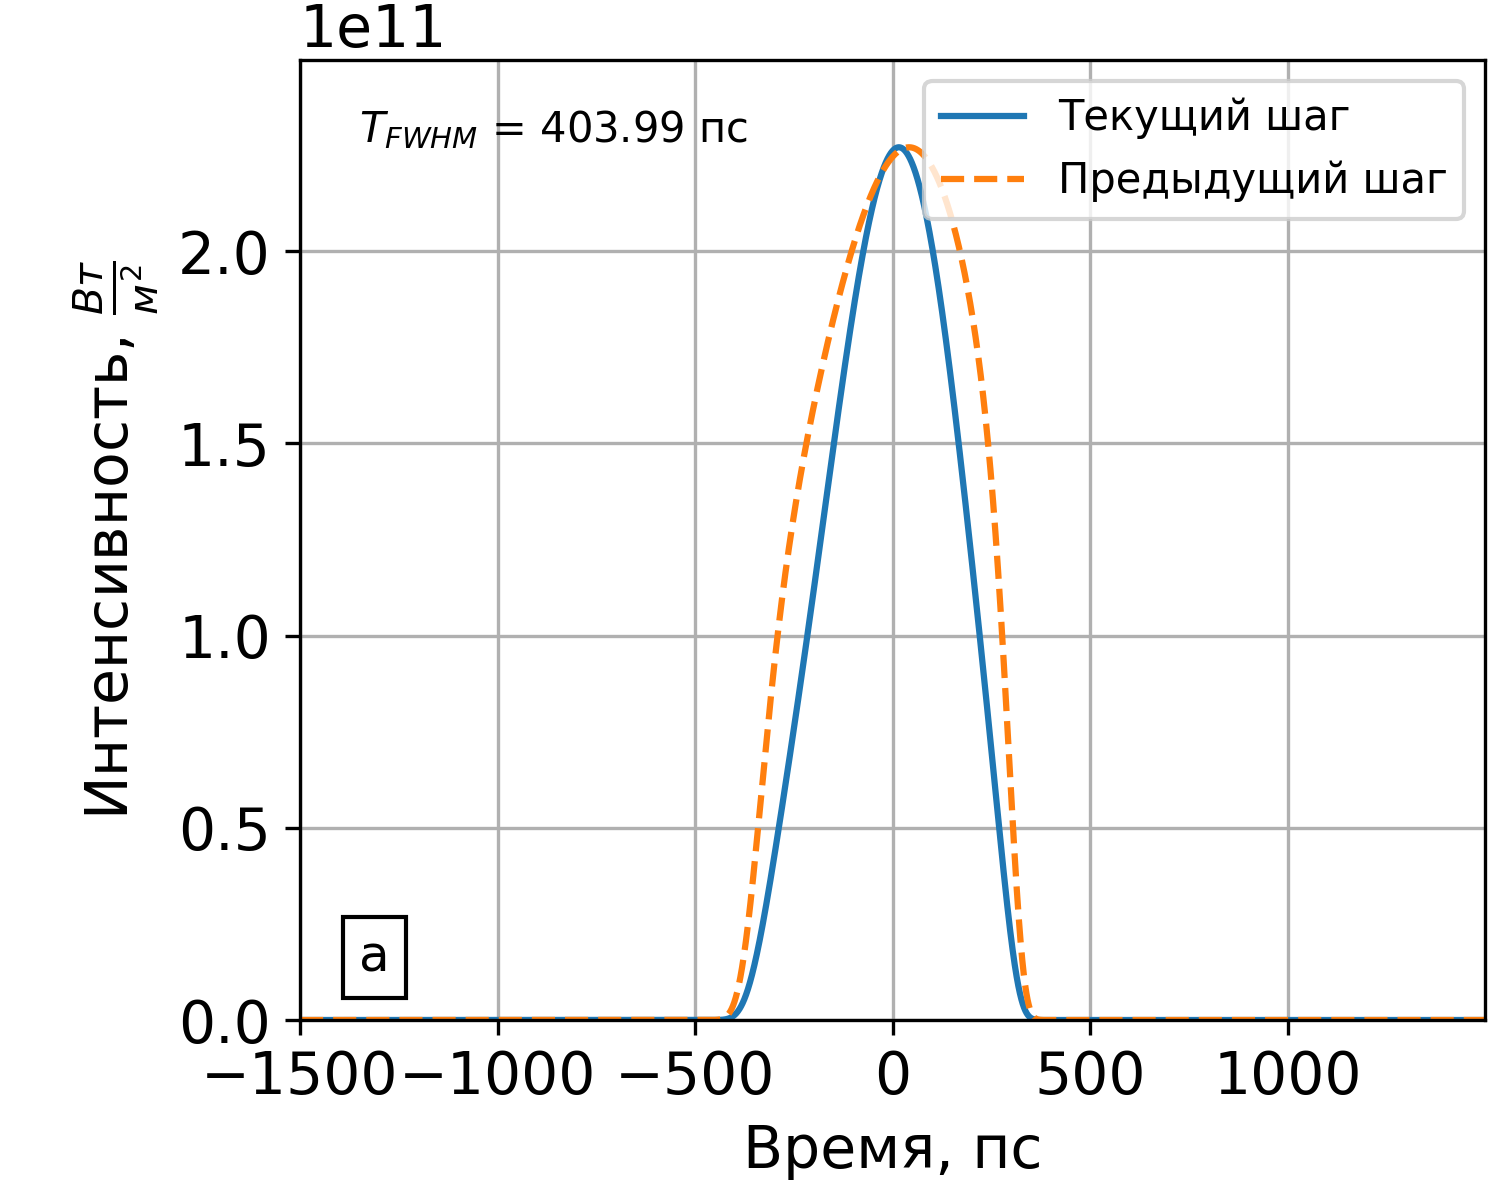
\includegraphics[width=\linewidth]{Images/Gauss Pulse Parabolic Profile/Импульс и спектр/!8. Yb3+ 6_125, 0.9m_pusle}
  \end{minipage}% <- % убирает хвостовой пробел / перевод строки
  \begin{minipage}[b]{0.5\textwidth}
    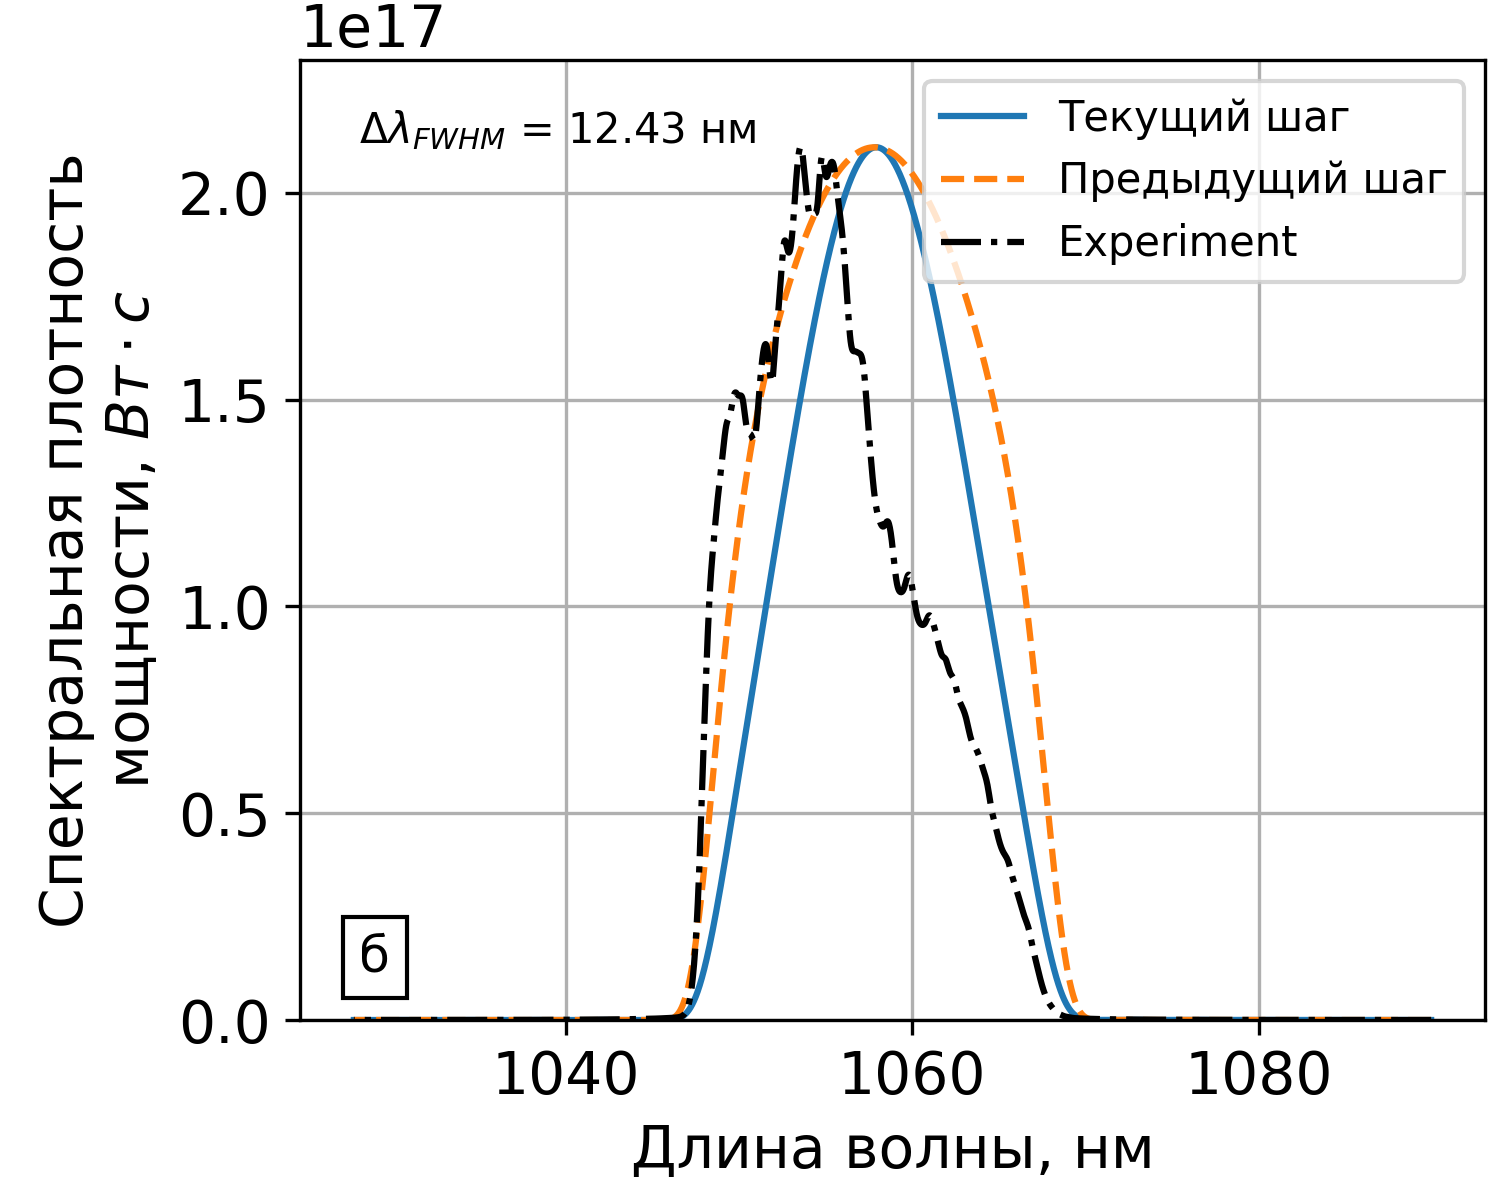
\includegraphics[width=\linewidth]{Images/Gauss Pulse Parabolic Profile/Импульс и спектр/!8. Yb3+ 6_125, 0.9m_spectrum}
  \end{minipage}

  \vspace{}

  \begin{minipage}[b]{0.5\textwidth}
    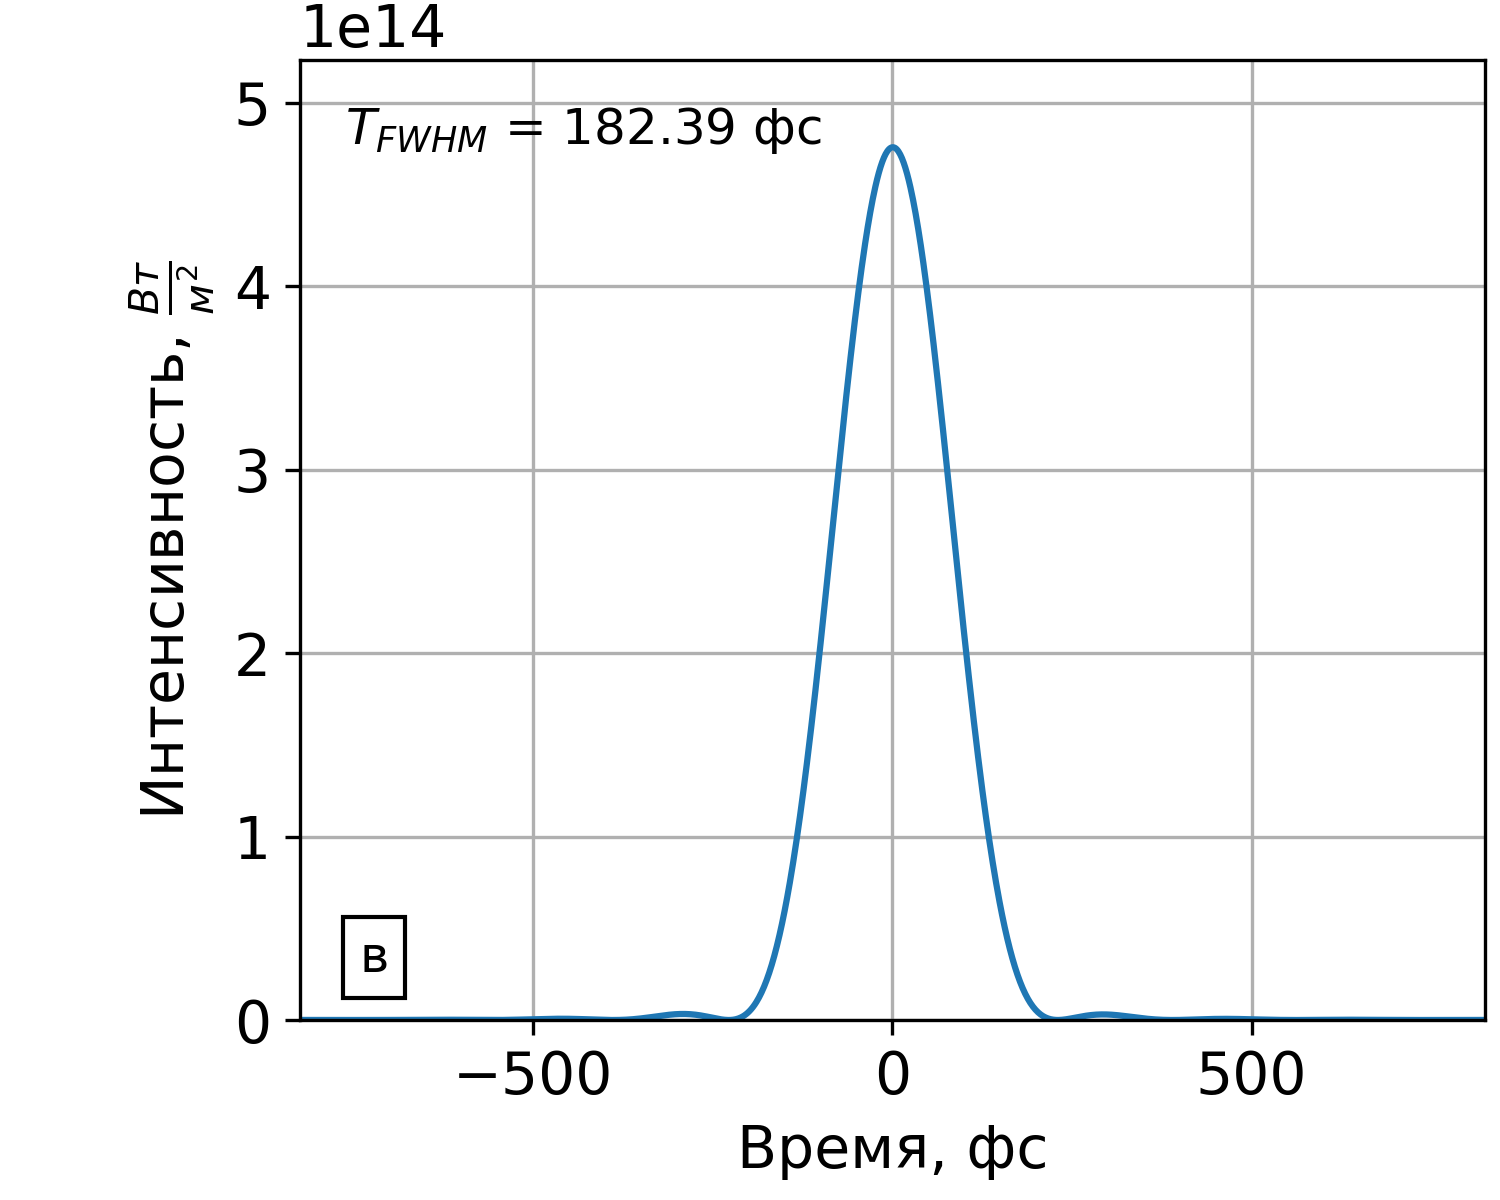
\includegraphics[width=\linewidth]{Images/Gauss Pulse Parabolic Profile/После компрессора/8 элемент gamma=49.49401 l_g=0.36732 сжатие}
  \end{minipage}% <- % убирает хвостовой пробел / перевод строки
  \begin{minipage}[b]{0.5\textwidth}
    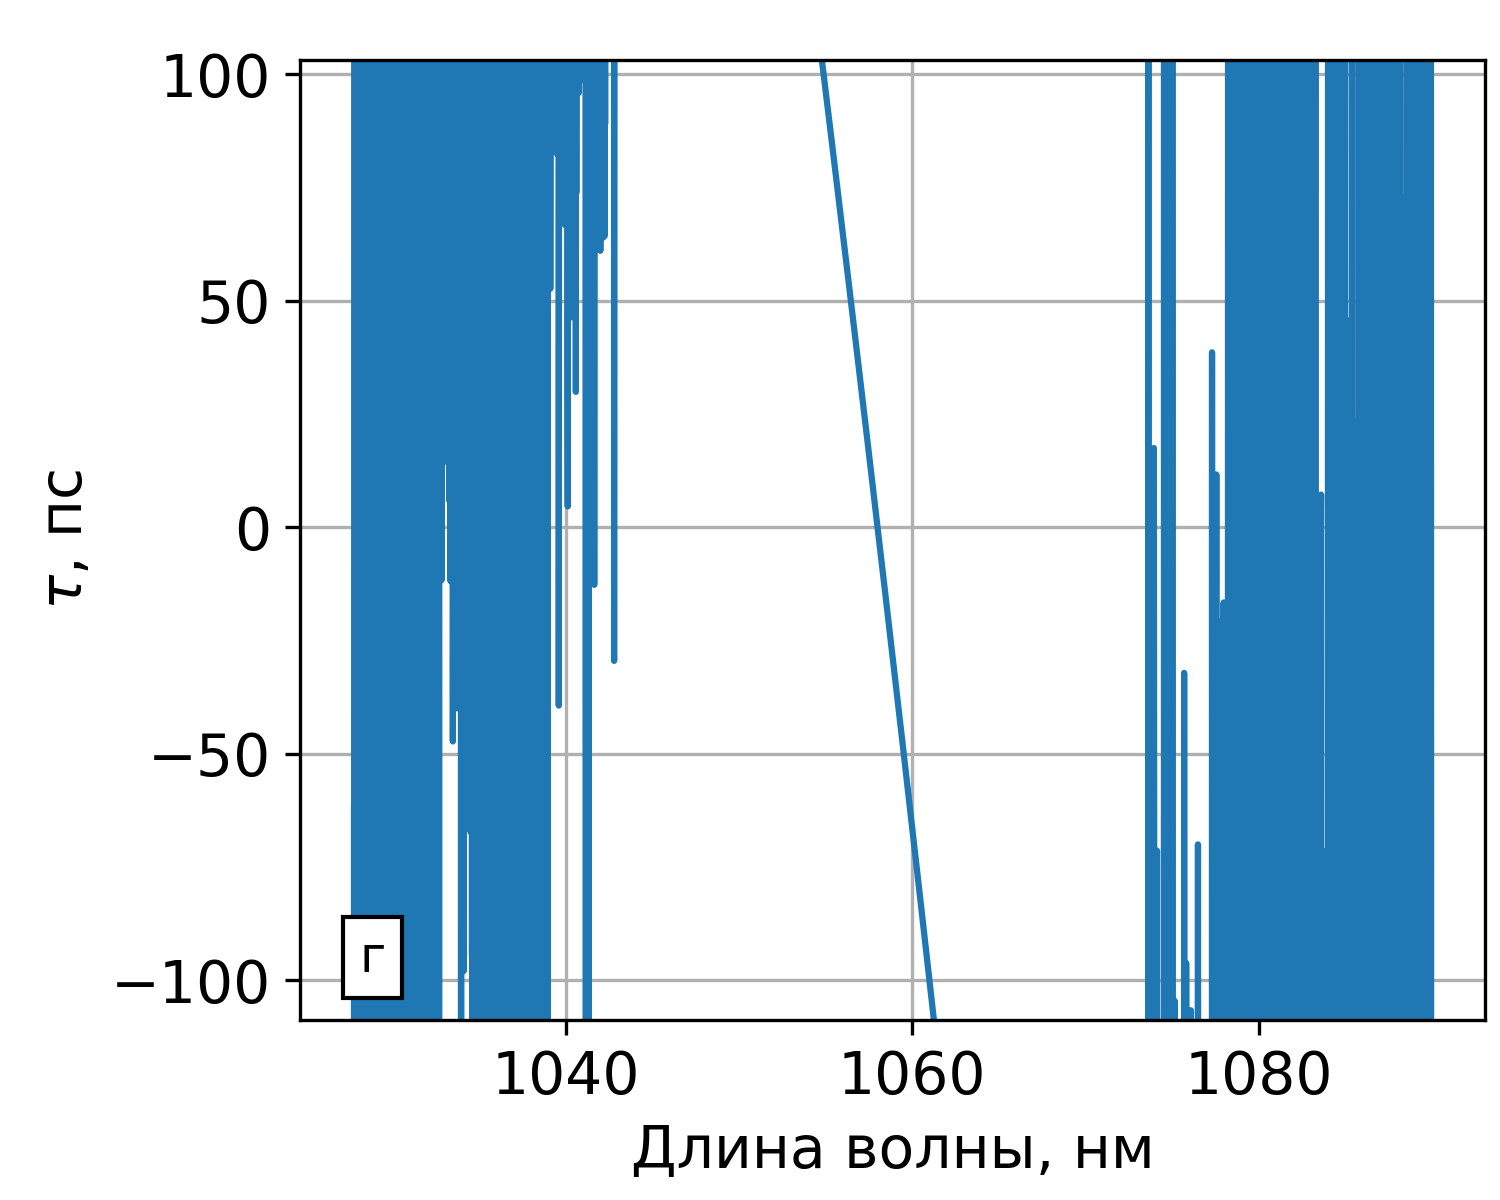
\includegraphics[width=\linewidth]{Images/Gauss Pulse Parabolic Profile/Импульс и спектр/!8. Yb3+ 6_125, 0.9m_time_delay}
  \end{minipage}

  \caption{Гауссов а) импульс, б) его спектр г) и групповая задержка после первого иттербиевого волокна (номер 5 на
  рисунке 2) с параболическим профилем усиления. Приведён график г) импульса, сжатого в решёточном компрессоре}
  \label{fig:both}
\end{figure}

Рассмотрим только поведение импульса после каскадов усиления. На рисунке 14 видно, что после первого иттербиевого
волокна импульс (рисунок 14в) сжимается практически идеально, параболический спектр усиления не меняет форму спектра
(рисунок 14б), а только незначительно сужает его, так как центр усиления находится на центральной частоте.
Соответственно боковые компоненты усиливаются слабее.

На рисунке 15 изображен импульс после второго каскада усиления. На спектре (рисунок 15б) видно, насколько сильно профиль
отличается от экспериментального. При этом импульс (рисунок 15в) сжимается практически идеально, боковые лепестки малы.
Длительность импульса увеличилась, что объясняется сужением спектра из-за усиления.

\begin{figure}[h!]
  \centering
  \begin{minipage}[b]{0.5\textwidth}
    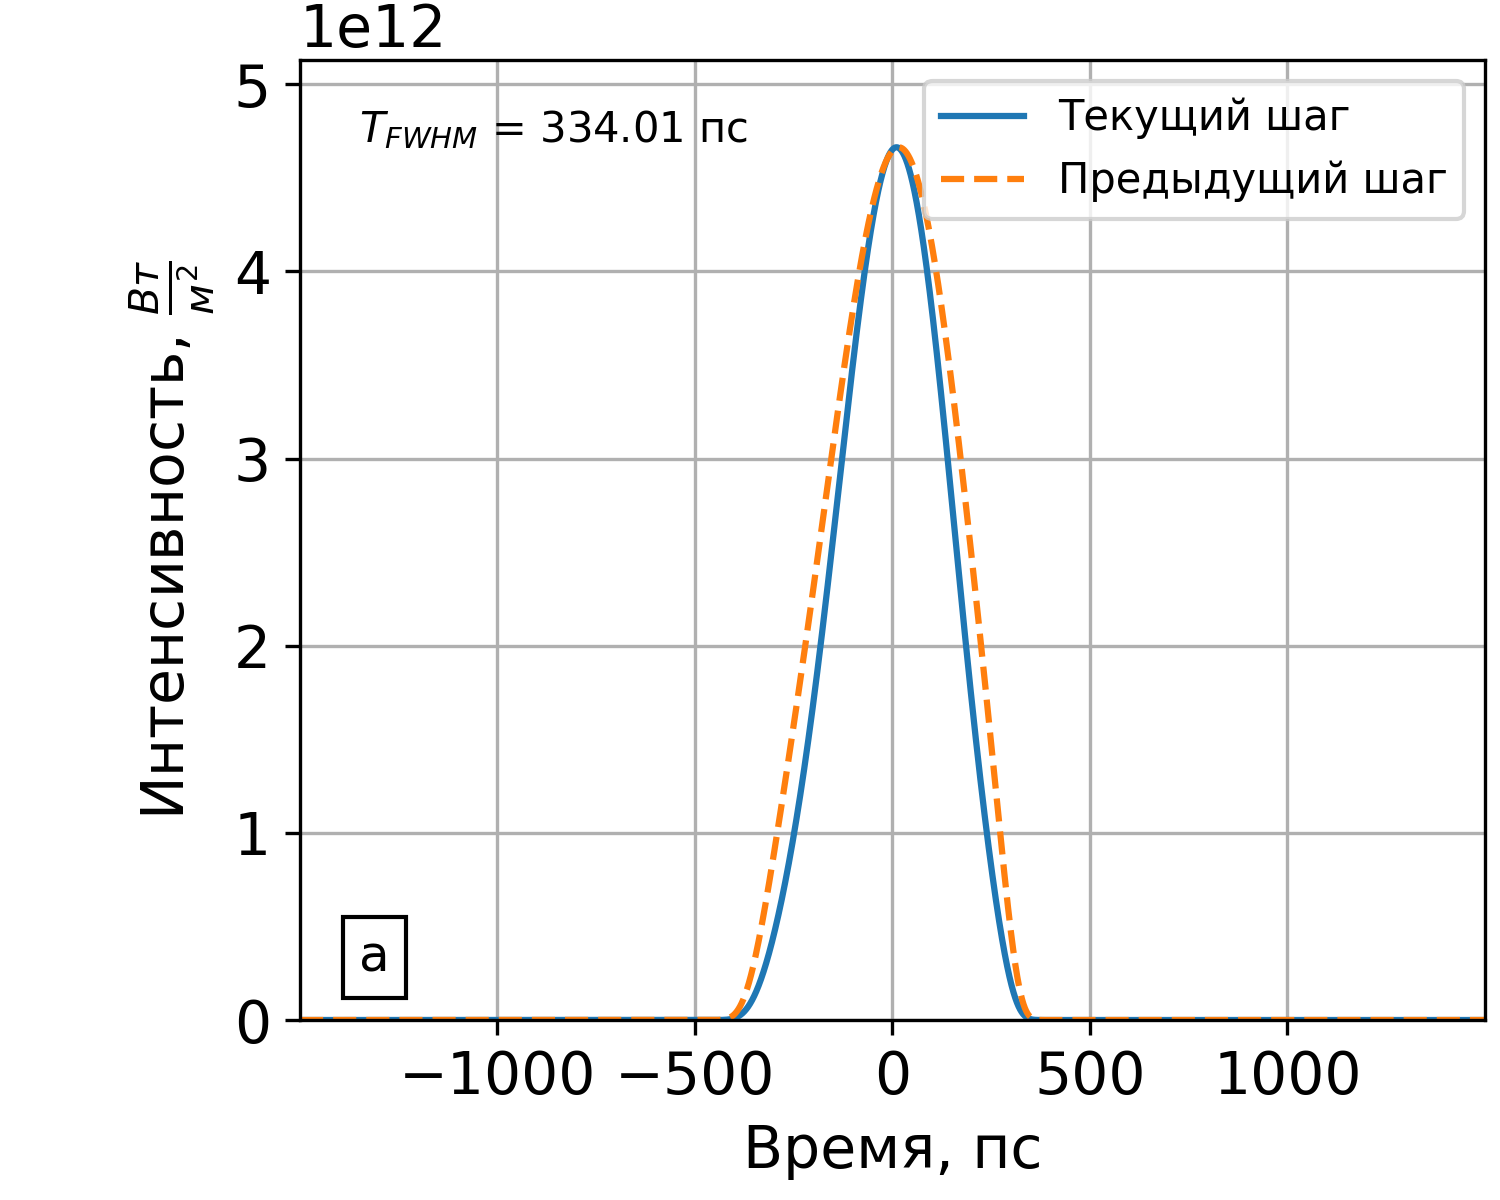
\includegraphics[width=\linewidth]{Images/Gauss Pulse Parabolic Profile/Импульс и спектр/!14. Yb3+ 6_125, 0.8m_pusle}
  \end{minipage}% <- % убирает хвостовой пробел / перевод строки
  \begin{minipage}[b]{0.5\textwidth}
    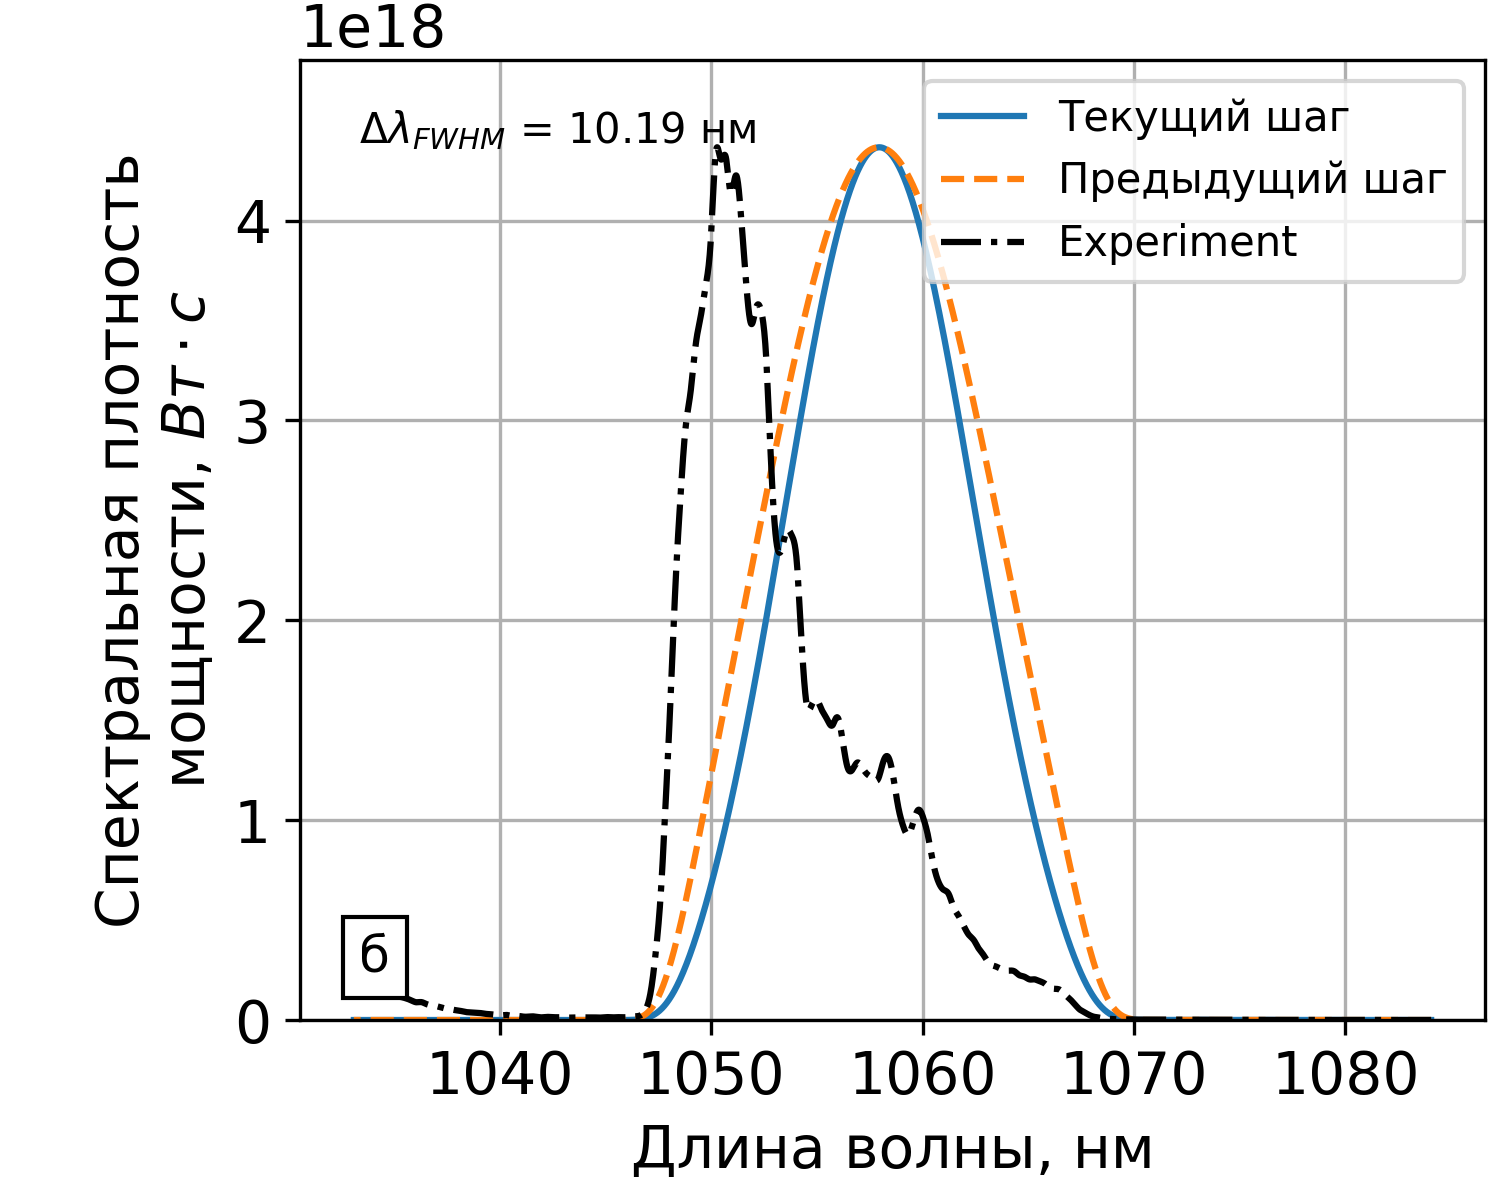
\includegraphics[width=\linewidth]{Images/Gauss Pulse Parabolic Profile/Импульс и спектр/!14. Yb3+ 6_125, 0.8m_spectrum}
  \end{minipage}

  \vspace{}

  \begin{minipage}[b]{0.5\textwidth}
    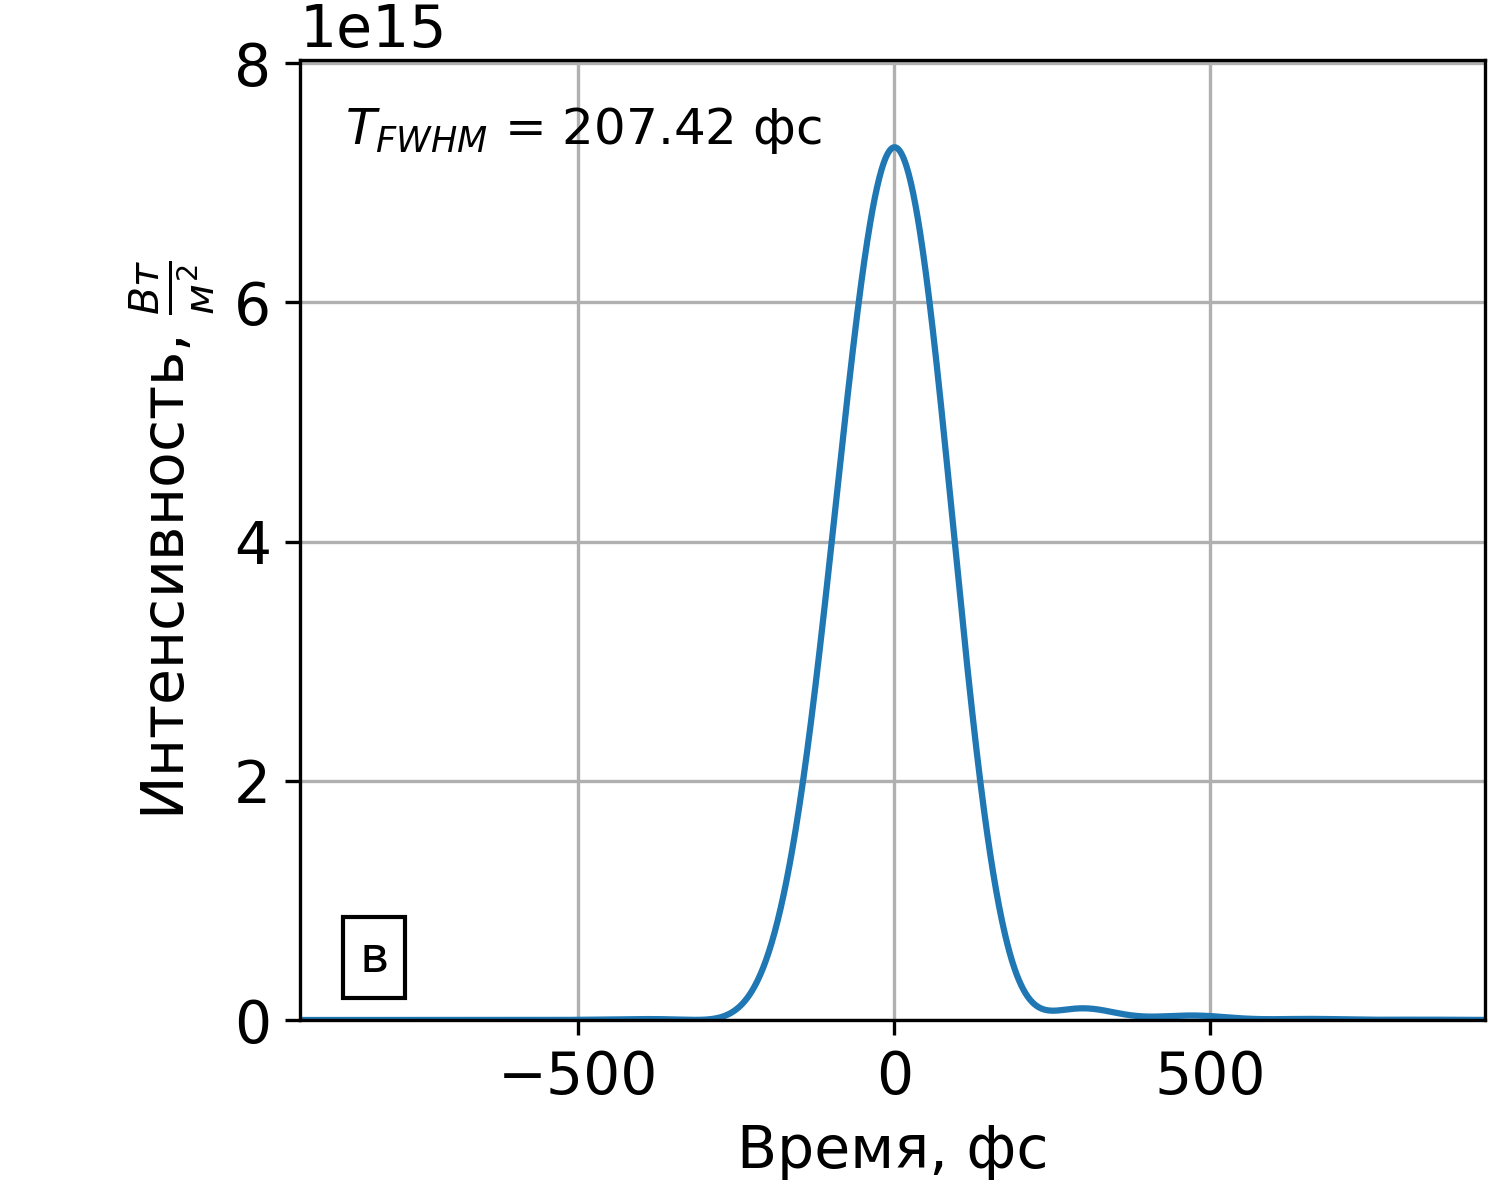
\includegraphics[width=\linewidth]{Images/Gauss Pulse Parabolic Profile/После компрессора/14 элемент gamma=49.60634 l_g=0.37317 сжатие}
  \end{minipage}% <- % убирает хвостовой пробел / перевод строки
  \begin{minipage}[b]{0.5\textwidth}
    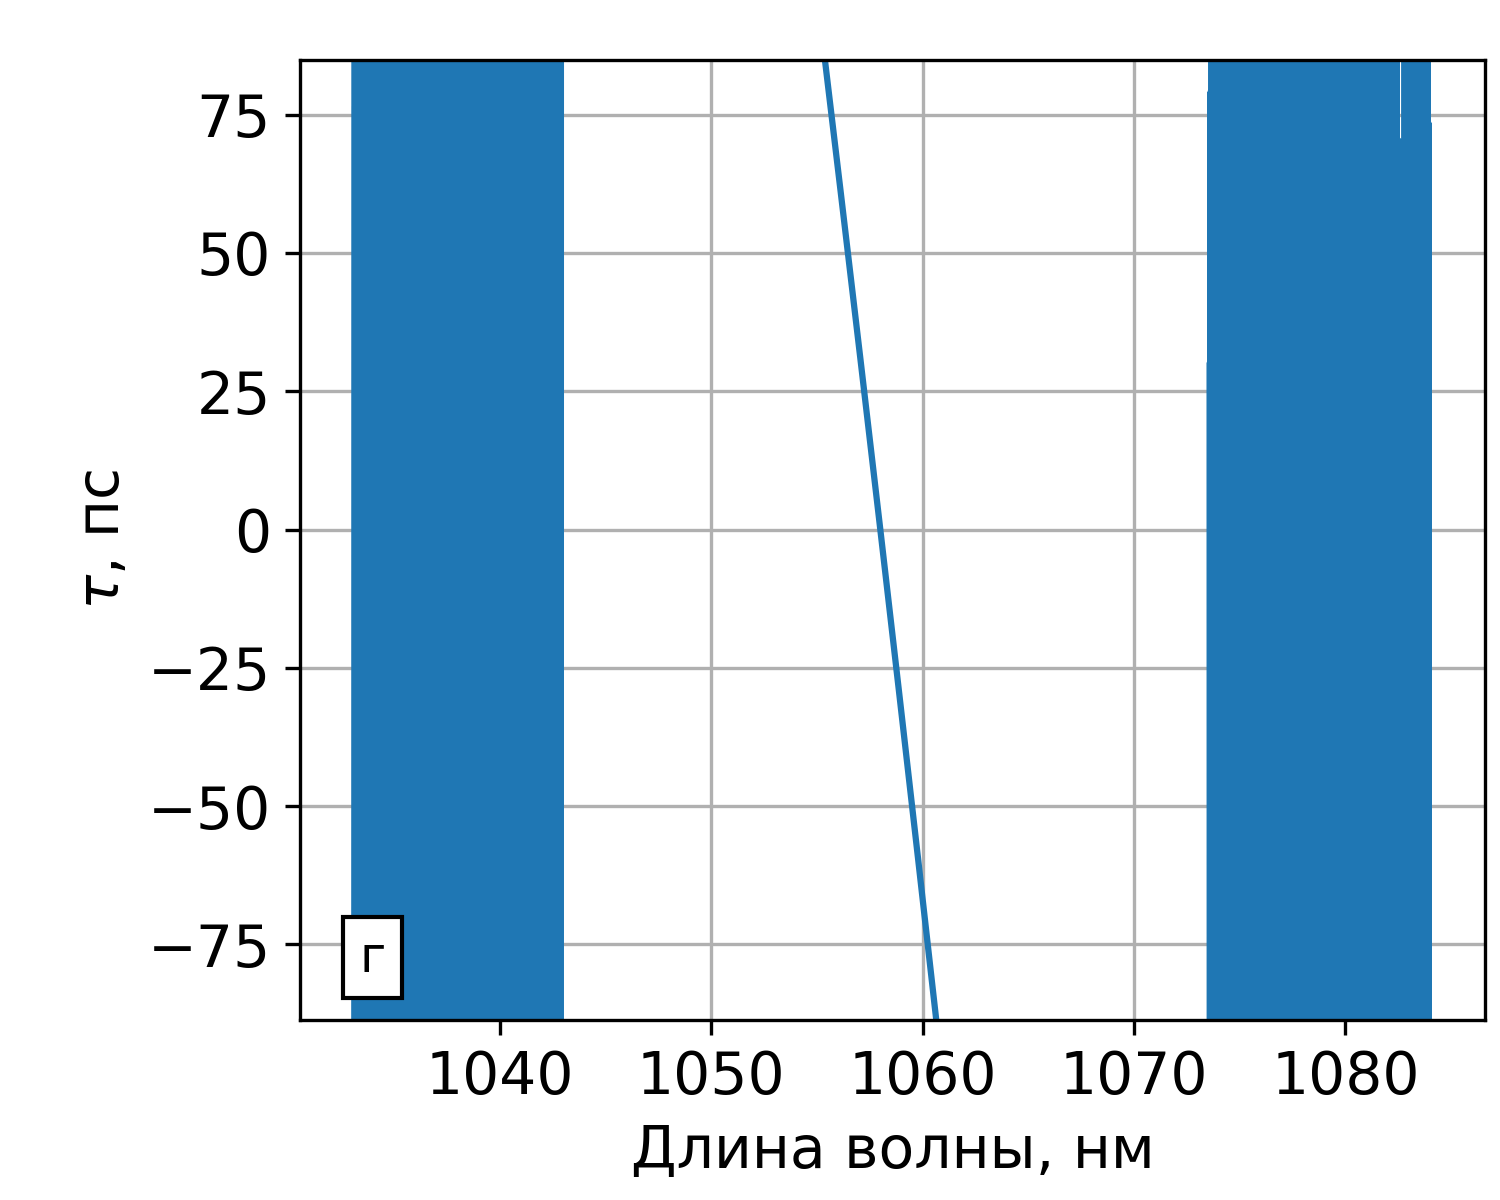
\includegraphics[width=\linewidth]{Images/Gauss Pulse Parabolic Profile/Импульс и спектр/!14. Yb3+ 6_125, 0.8m_time_delay}
  \end{minipage}

  \caption{Гауссов а) импульс, б) его спектр г) и групповая задержка после второго иттербиевого волокна (номер 7 на
  рисунке 2) с параболическим профилем усиления. Приведён график г) импульса, сжатого в решёточном компрессоре}
  \label{fig:both}
\end{figure}

На рисунке 16 изображён импульс после последнего каскада усиления и итогового сжатия в компрессоре. На рисунке 16в
видны осцилляции (1.5\% энергии импульса), которые обусловлены не компенсированными четвёртым и выше порядками дисперсии. Как отмечалось выше,
$\beta_4$ и $\beta_5$ сейчас описываются с помощью введённой поправки, которая является константой. Поэтому поведение
реальных решёток в компрессоре может вносить эти порядки дисперсии в фазу по-другому.

\begin{figure}[h!]
  \centering
  \begin{minipage}[b]{0.5\textwidth}
    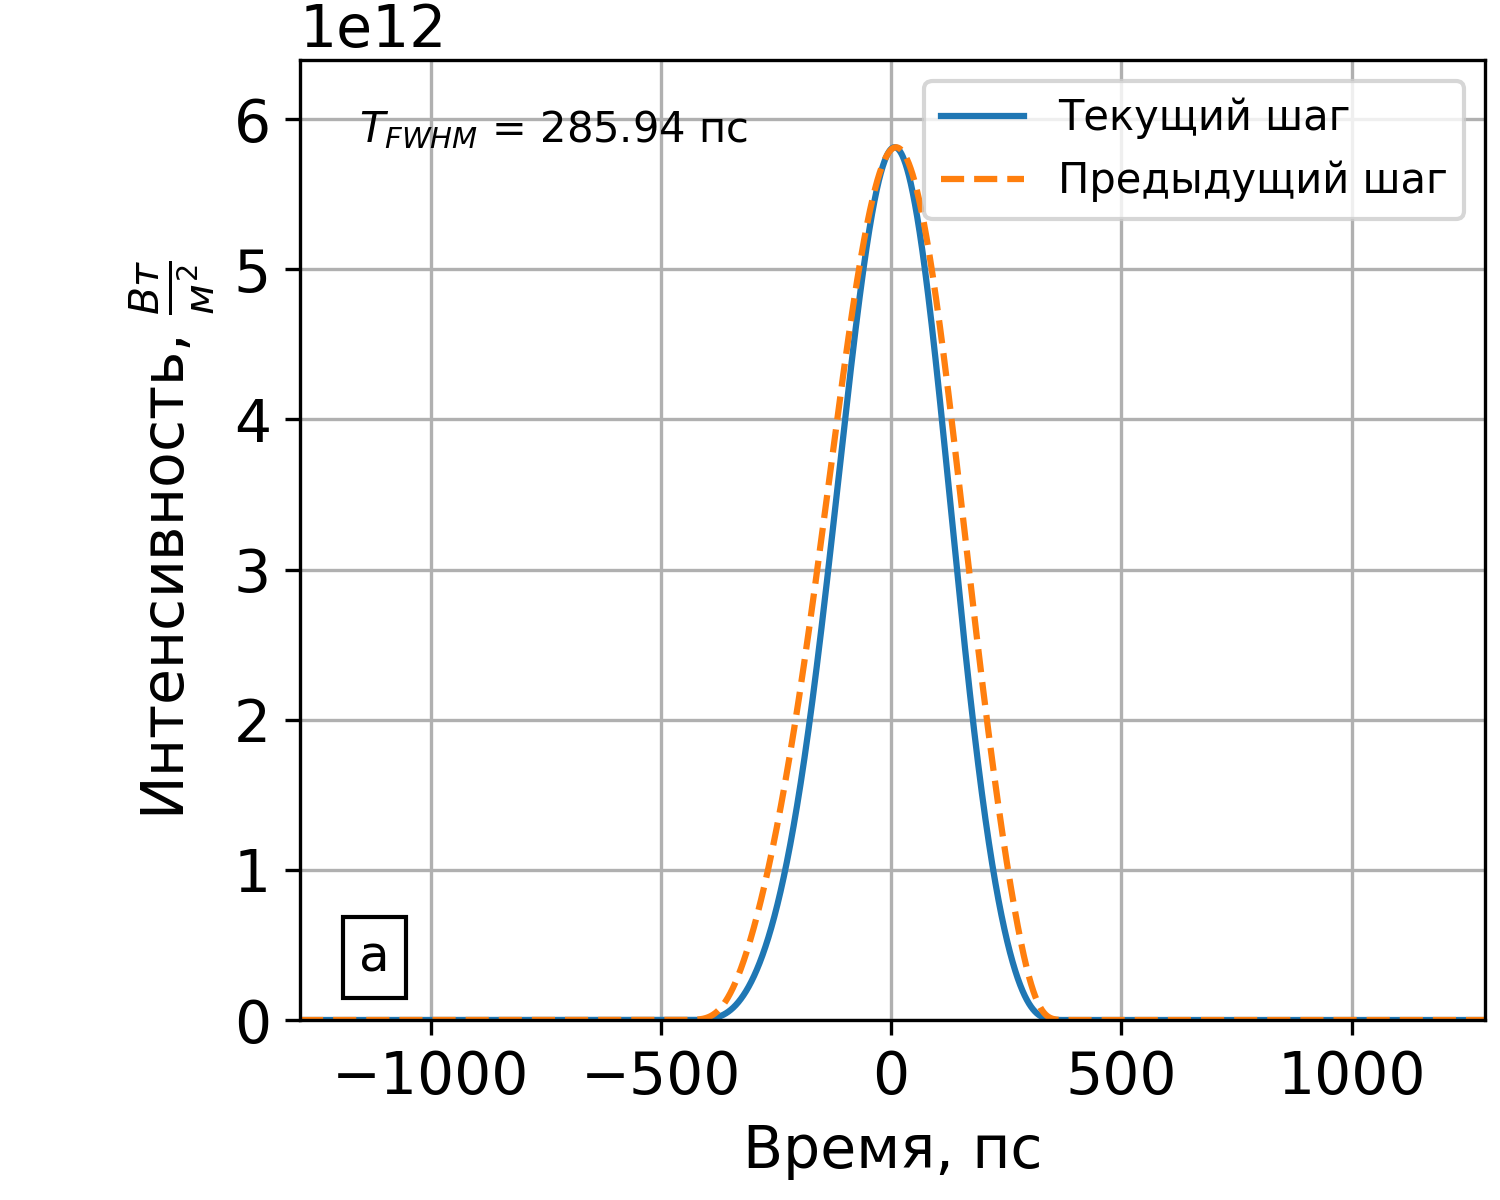
\includegraphics[width=\linewidth]{Images/Gauss Pulse Parabolic Profile/Импульс и спектр/!23. Fiber_pusle}
  \end{minipage}% <- % убирает хвостовой пробел / перевод строки
  \begin{minipage}[b]{0.5\textwidth}
    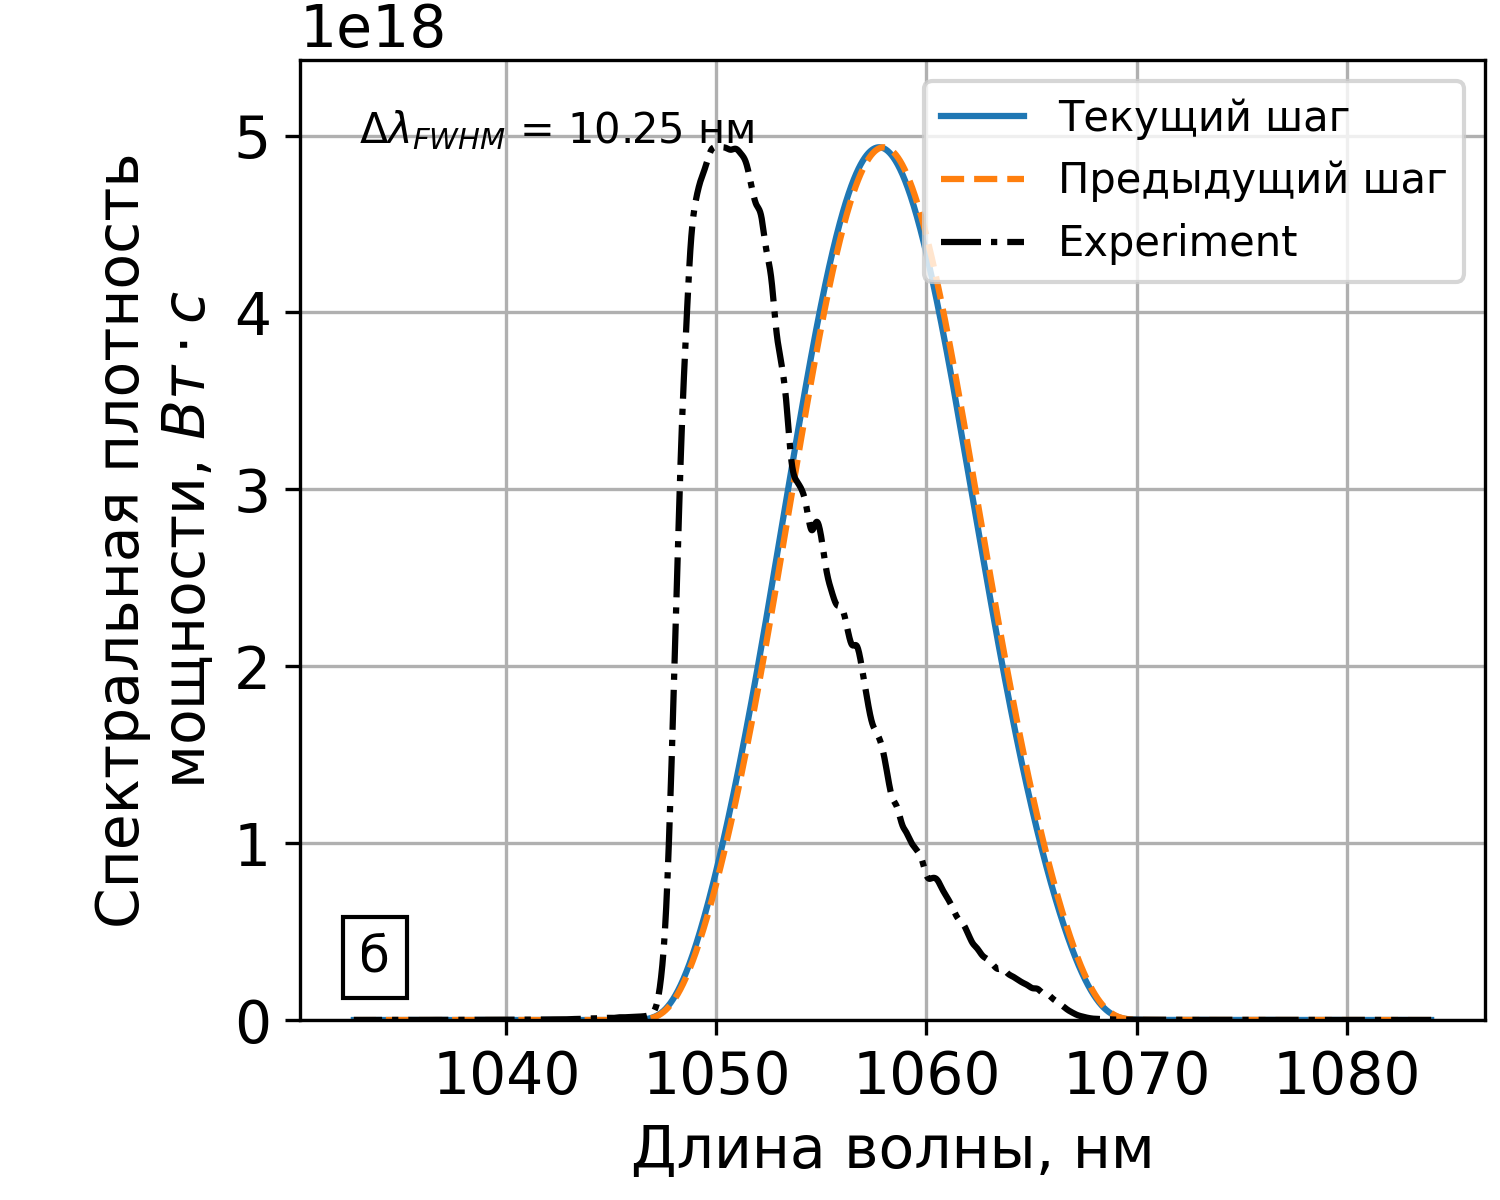
\includegraphics[width=\linewidth]{Images/Gauss Pulse Parabolic Profile/Импульс и спектр/!23. Fiber_spectrum}
  \end{minipage}

  \vspace{}

  \begin{minipage}[b]{0.5\textwidth}
    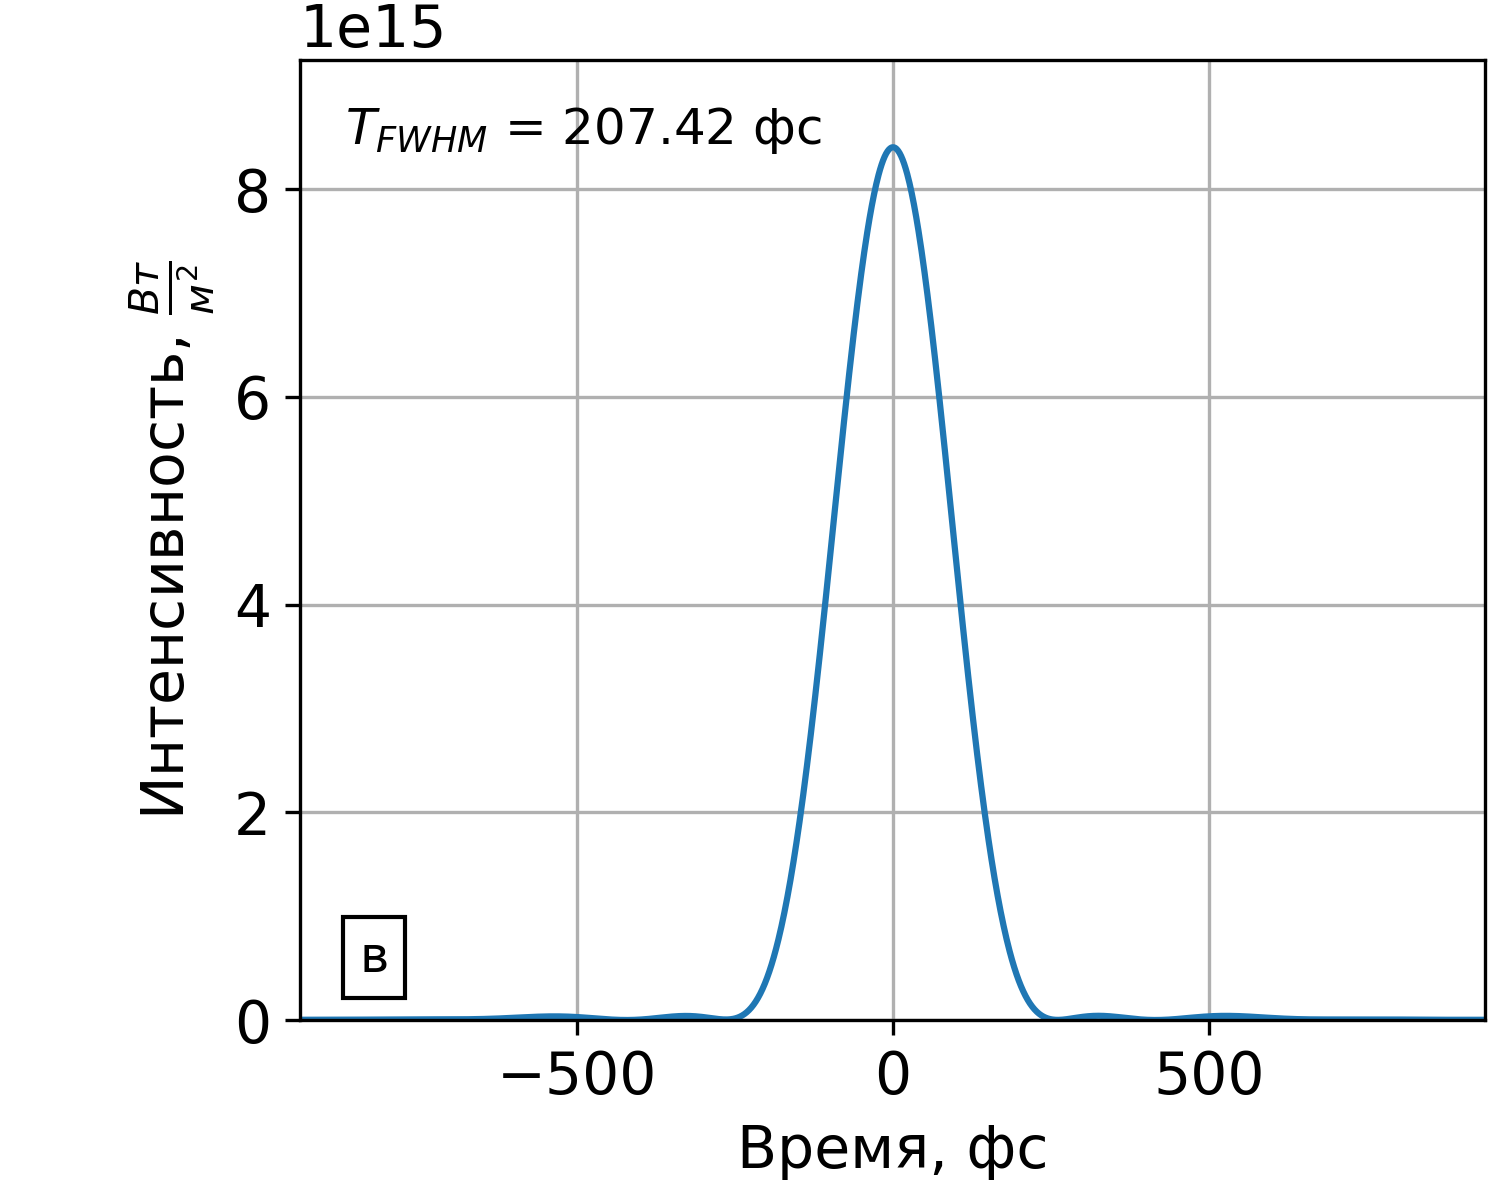
\includegraphics[width=\linewidth]{Images/Gauss Pulse Parabolic Profile/После компрессора/23 элемент gamma=49.59073 l_g=0.37532 сжатие}
  \end{minipage}% <- % убирает хвостовой пробел / перевод строки
  \begin{minipage}[b]{0.5\textwidth}
    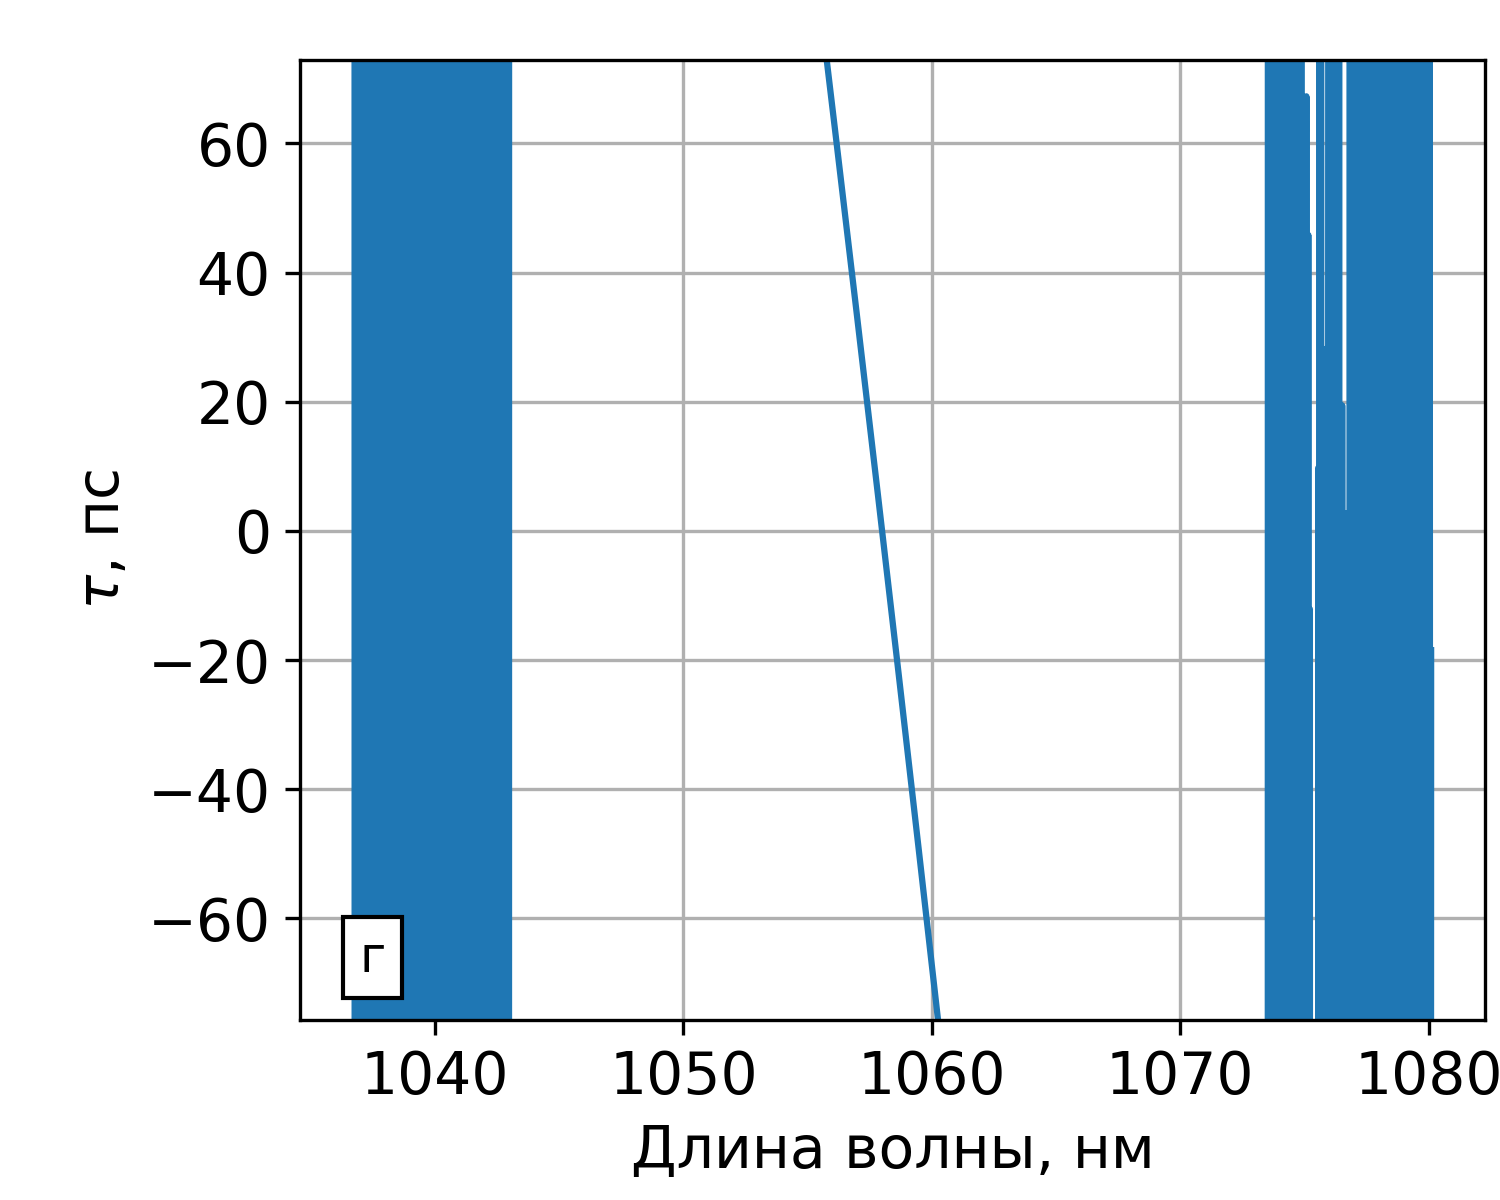
\includegraphics[width=\linewidth]{Images/Gauss Pulse Parabolic Profile/Импульс и спектр/!23. Fiber_time_delay}
  \end{minipage}

  \caption{Гауссов а) импульс, б) его спектр г) и групповая задержка после третьего иттербиевого волокна (номер 7 на
  рисунке 2) с параболическим профилем усиления. Приведён график г) импульса, сжатого в решёточном компрессоре}
  \label{fig:both}
\end{figure}

На рисунке 17 представлен график изменения $\beta_3$ на каждом элементе схемы. Вновь можно обратить внимание, что после
второго каскада усиления (элемент 7) увеличивается вклад волокон в модуляцию фазы. Но самое интересное, что $\beta_3$
меняет знак по сравнению с рисунком 11 для профиля усиления $Yb^{3+}$. Из-за сильной асимметрии профиля усиления,
приводящей к асимметрии временной формы и спектра импульса, нелинейные эффекты модулируют фазу, поэтому значения $\beta_3$
сильно меняются. Такая же ситуация наблюдается и для $\beta_4$ на рисунке 18 в сравнении с рисунком 12.

\begin{figure}[h!]
    \centering
    \begin{minipage}[b]{0.5\textwidth}
        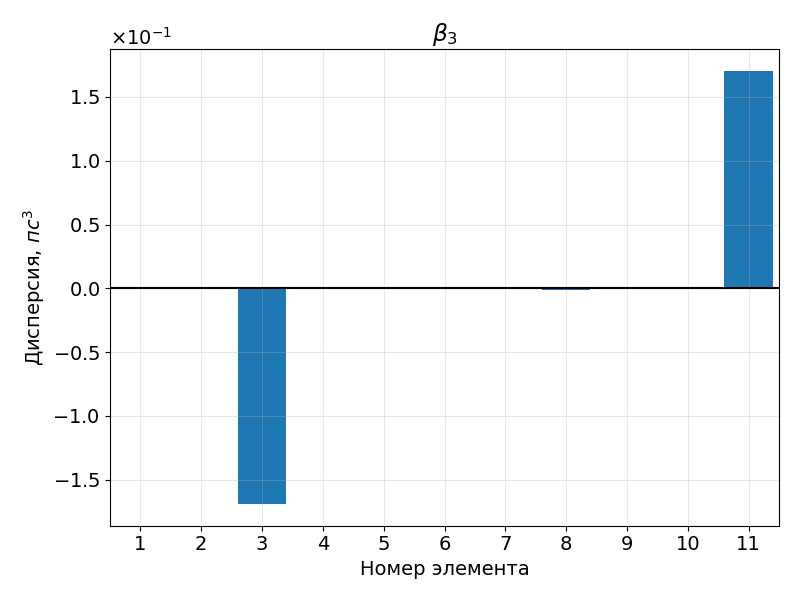
\includegraphics[width=\linewidth]{Images/Gauss Pulse Parabolic Profile/Беты/beta_3_full}
    \end{minipage}% <- % убирает хвостовой пробел / перевод строки
    \begin{minipage}[b]{0.5\textwidth}
        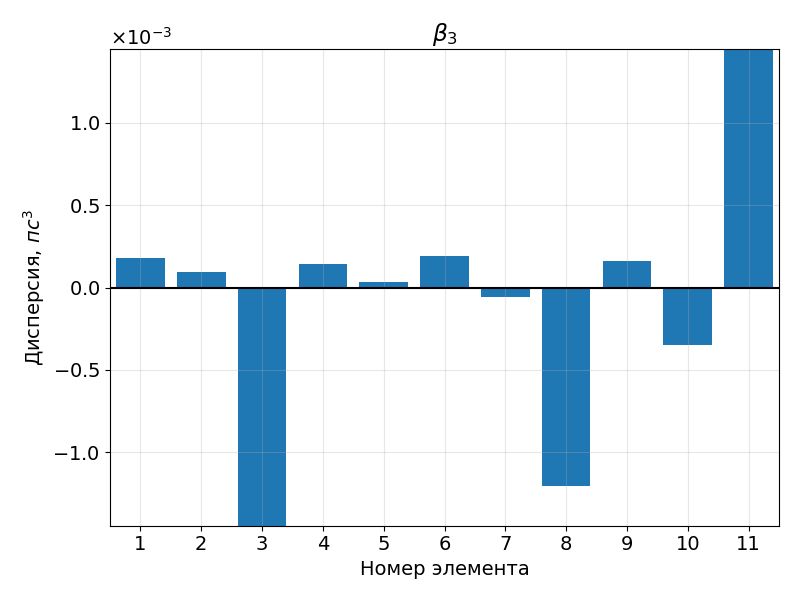
\includegraphics[width=\linewidth]{Images/Gauss Pulse Parabolic Profile/Беты/beta_3_cut}
    \end{minipage}

    \caption{Коэффициенты $\beta_3$, рассчитанные с помощью аппроксимации спектальной фазы полиномом,
     в двух масштабах (слева общий масштаб, справа увеличенный)}
    \label{fig:both}
\end{figure}

\begin{figure}[h!]
    \centering
    \begin{minipage}[b]{0.5\textwidth}
        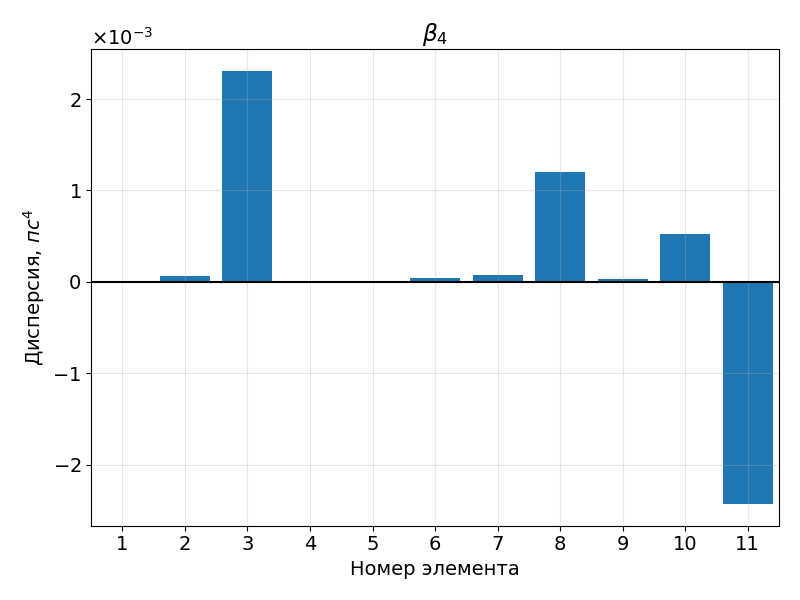
\includegraphics[width=\linewidth]{Images/Gauss Pulse Parabolic Profile/Беты/beta_4_full}
    \end{minipage}% <- % убирает хвостовой пробел / перевод строки
    \begin{minipage}[b]{0.5\textwidth}
        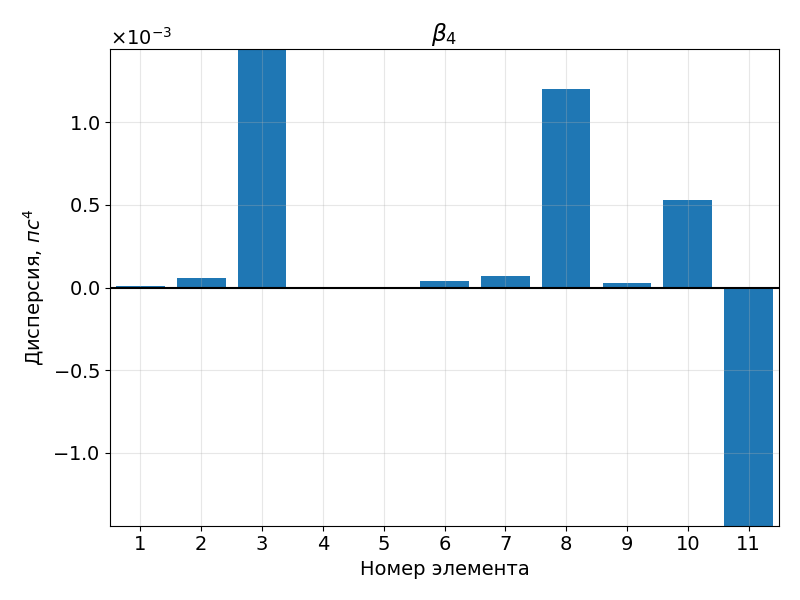
\includegraphics[width=\linewidth]{Images/Gauss Pulse Parabolic Profile/Беты/beta_4_cut}
    \end{minipage}

    \caption{Коэффициенты $\beta_4$, рассчитанные с помощью аппроксимации спектальной фазы полиномом,
     в двух масштабах (слева общий масштаб, справа увеличенный)}
    \label{fig:both}
\end{figure}

\subsection{Моделирование схемы с увеличенной длиной волокна}

Чтобы проверить, как длина волокна, а следовательно, и величина $B$-интеграла, влияют на способность импульса к сжатию,
длина волокна (номер 8 на рисунке) после второго каскада усиления была увеличена с 6.1 до 22.75 м. Так как изменения
способности сжатия будут видны только после третьего каскада усиления, то есть уже на выходе из оптической установки, мы
рассмотрим только их. На рисунке 19 приведён график импульса после последнего волокна. На рисунке 19в видно, что набег
фазы становится настолько огромным, что сжать импульс не получается.

\begin{figure}[h!]
  \centering
  \begin{minipage}[b]{0.5\textwidth}
    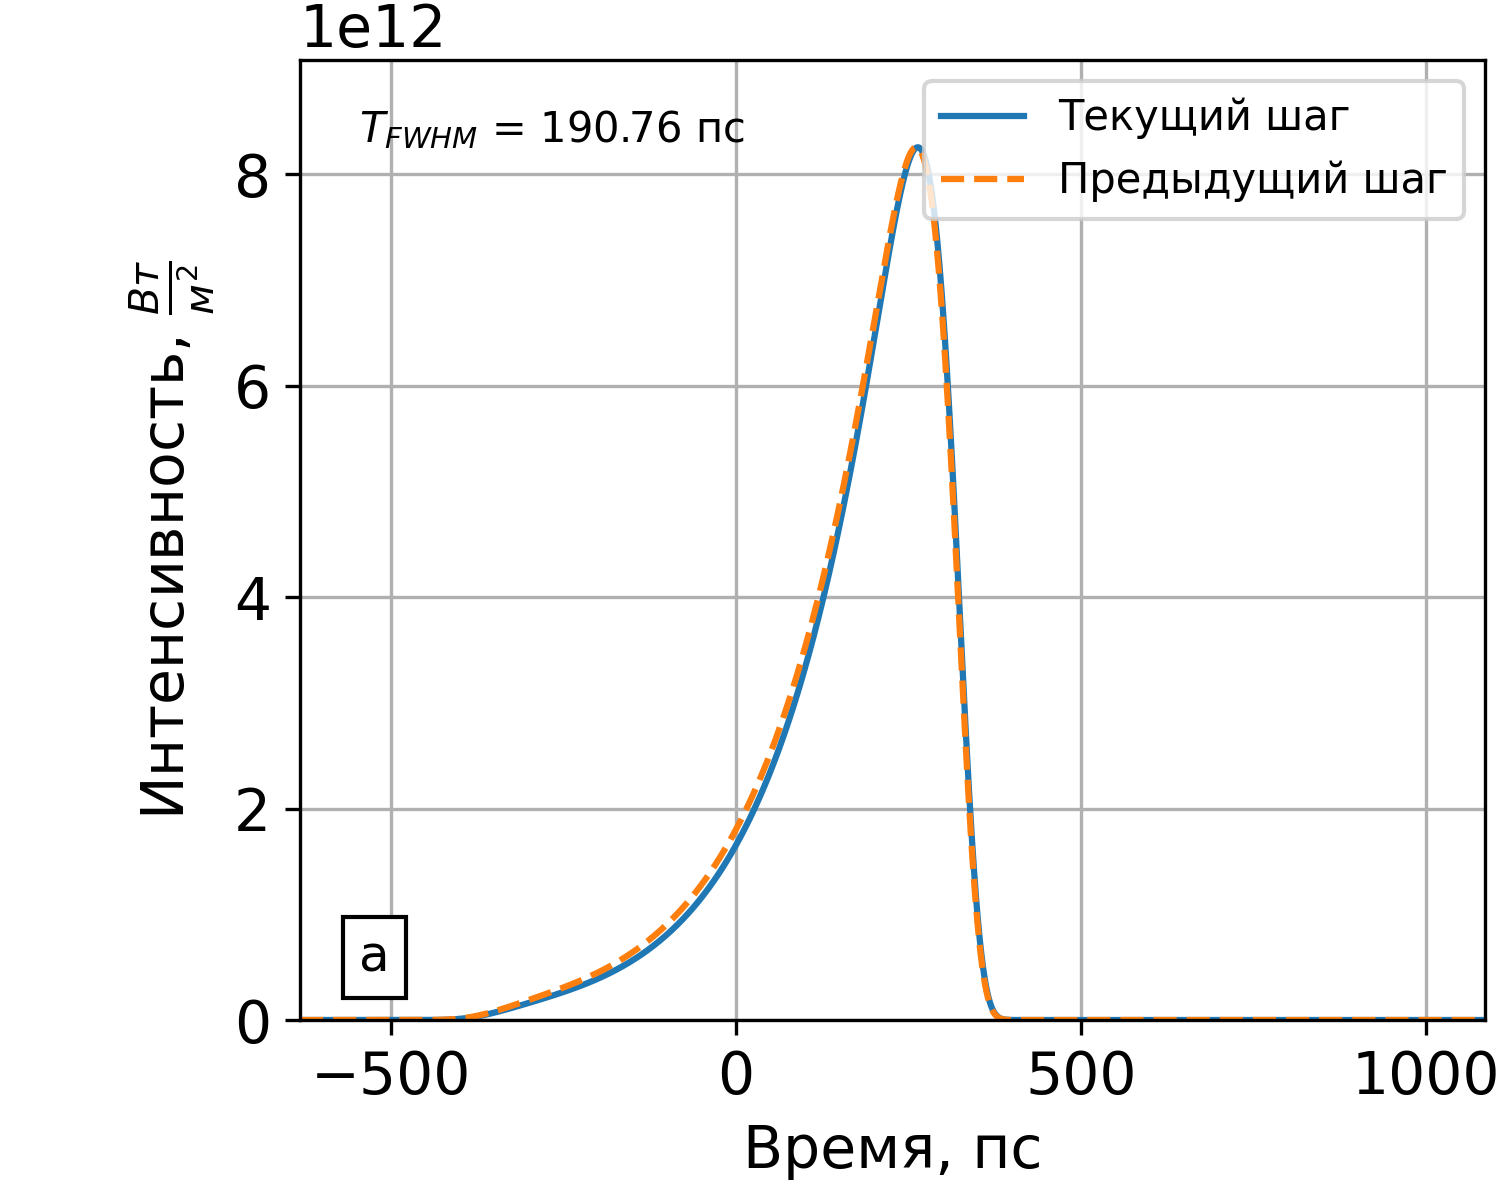
\includegraphics[width=\linewidth]{Images/Gauss Pulse x10/!23. Fiber_pusle}
  \end{minipage}% <- % убирает хвостовой пробел / перевод строки
  \begin{minipage}[b]{0.5\textwidth}
    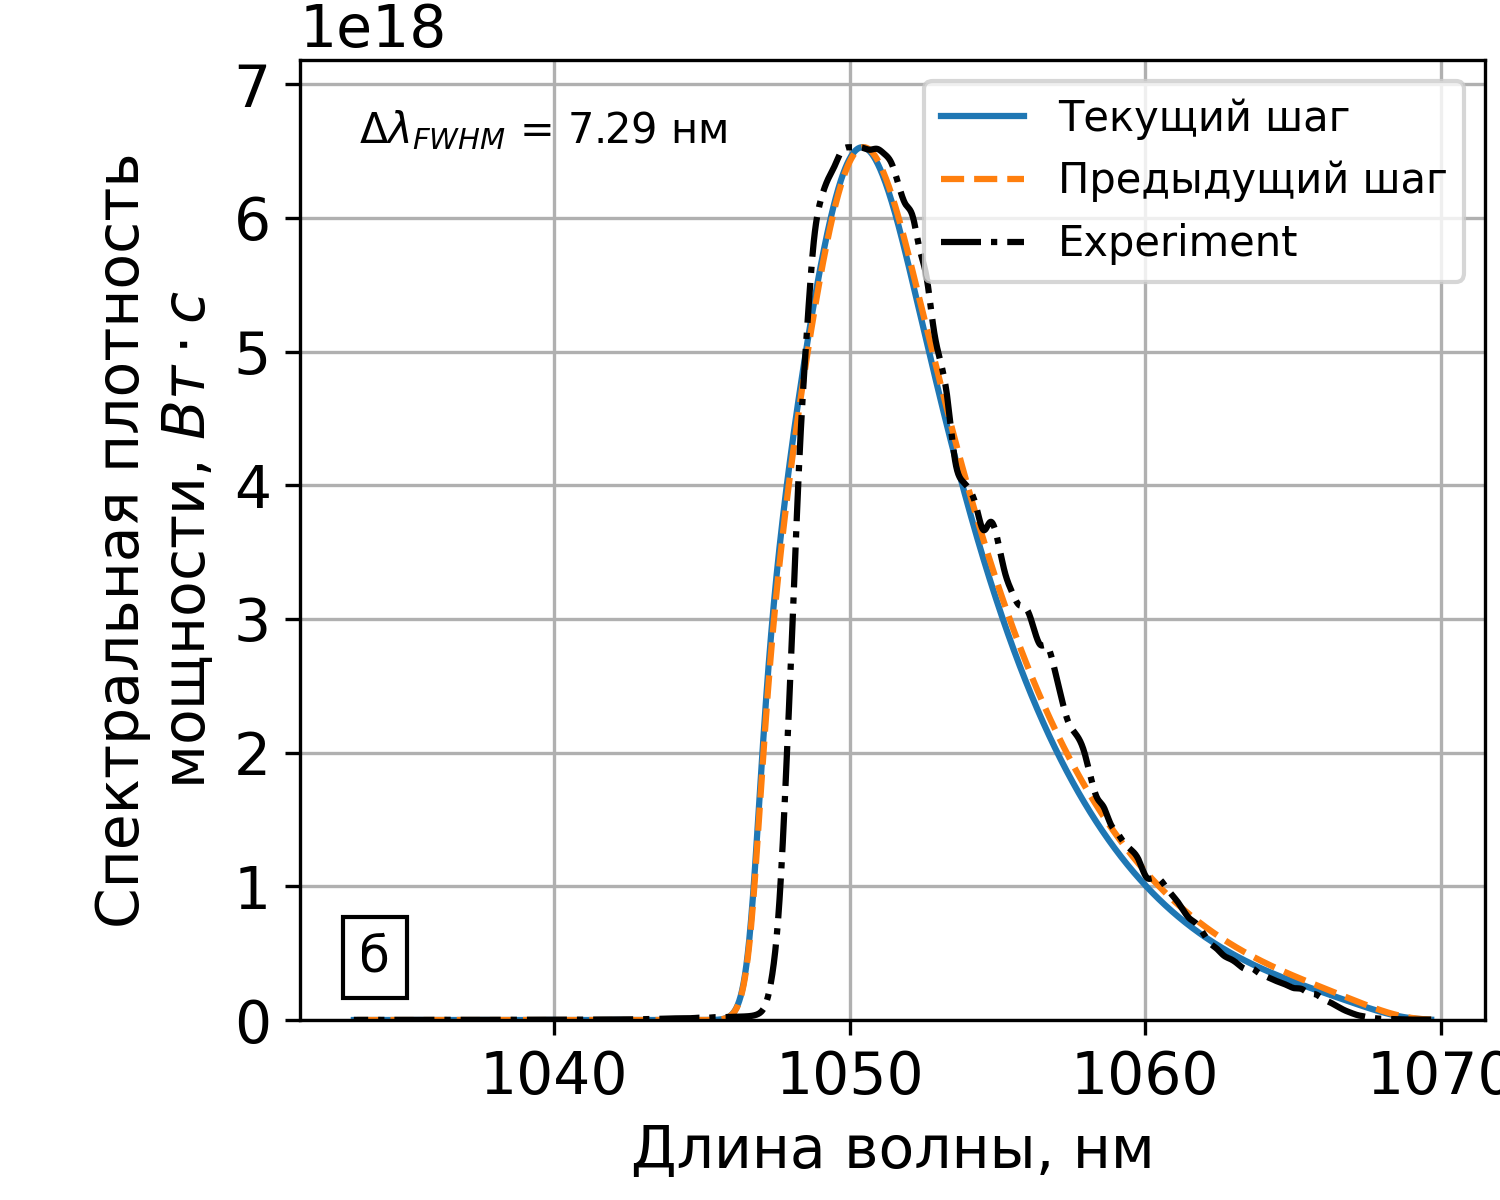
\includegraphics[width=\linewidth]{Images/Gauss Pulse x10/!23. Fiber_spectrum}
  \end{minipage}

  \vspace{}

  \begin{minipage}[b]{0.5\textwidth}
    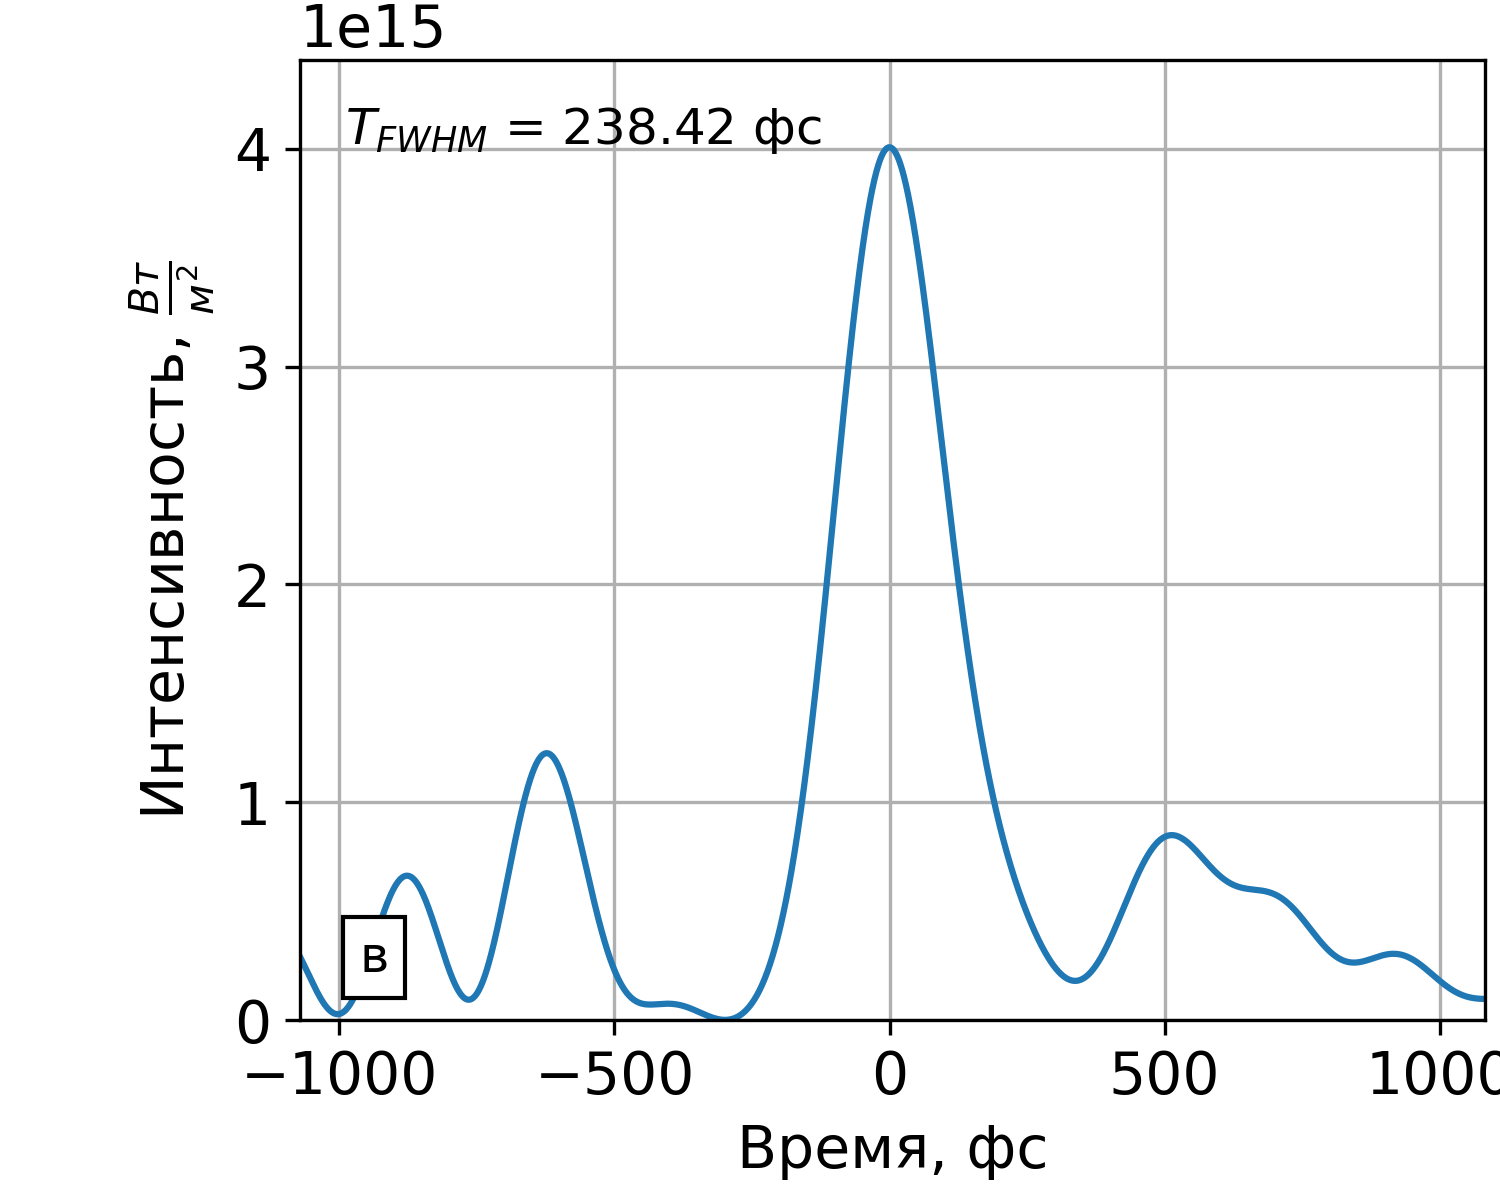
\includegraphics[width=\linewidth]{Images/Gauss Pulse x10/23 элемент gamma=60.88315 l_g=0.73684 сжатие}
  \end{minipage}% <- % убирает хвостовой пробел / перевод строки
  \begin{minipage}[b]{0.5\textwidth}
    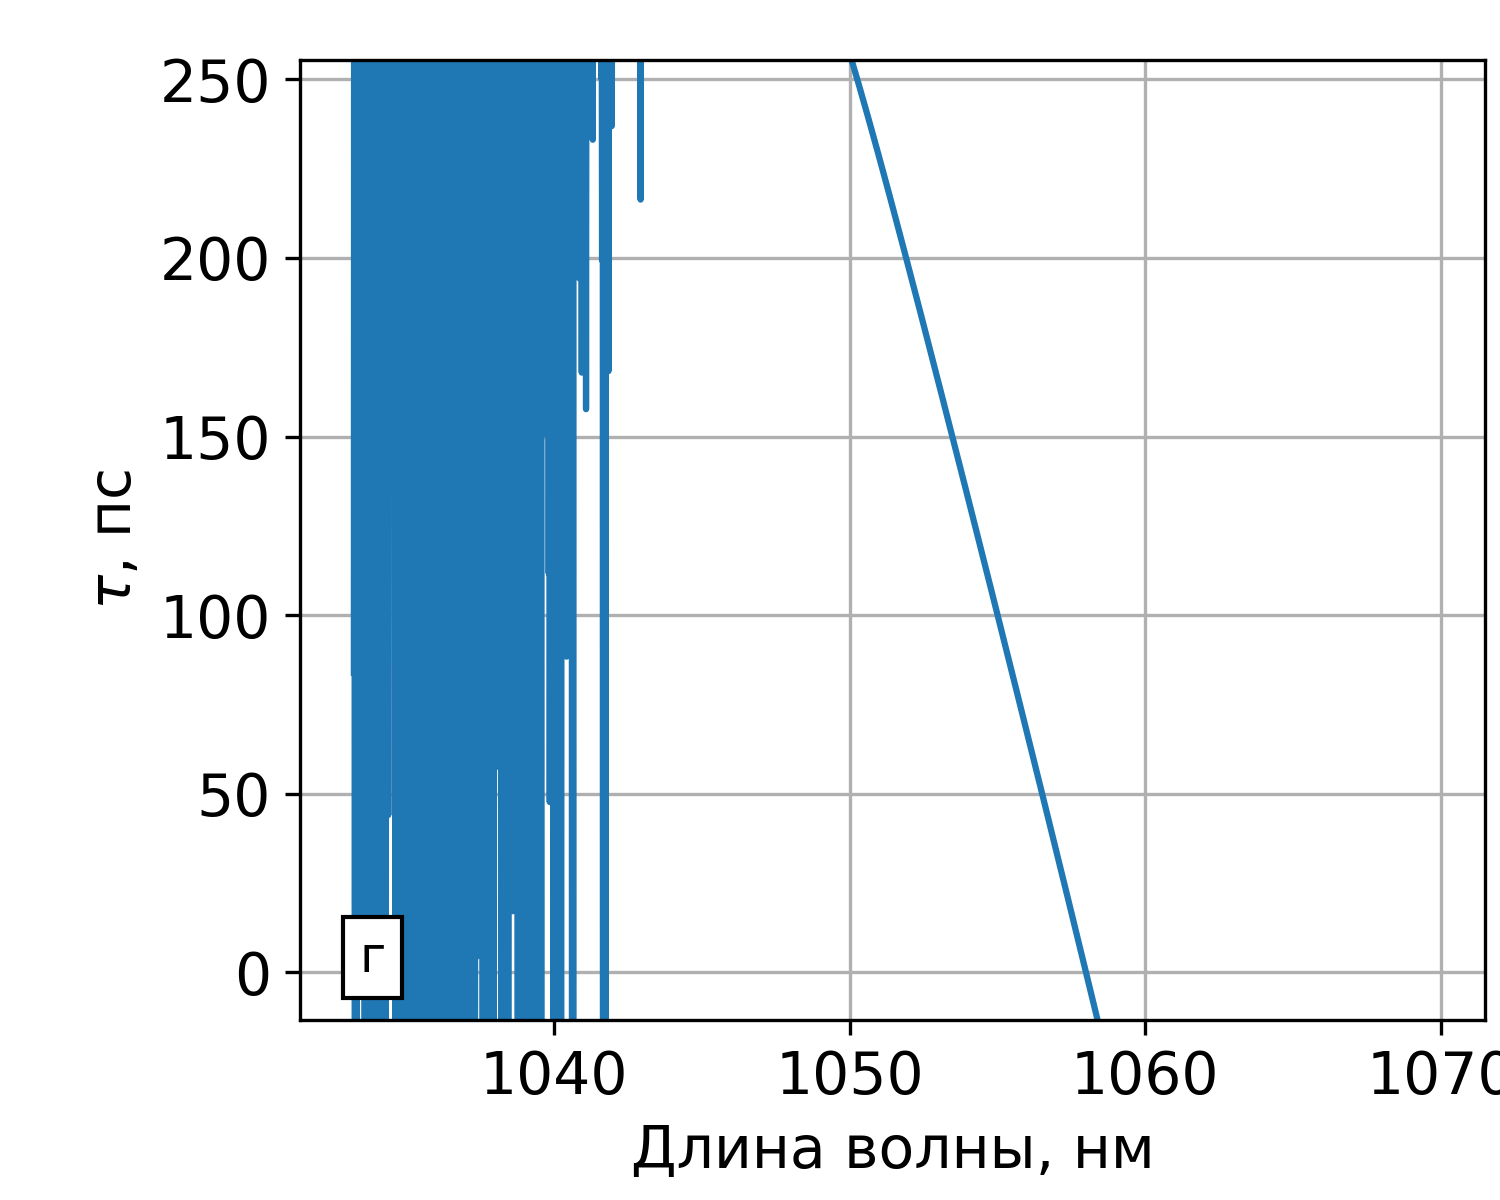
\includegraphics[width=\linewidth]{Images/Gauss Pulse x10/!23. Fiber_time_delay}
  \end{minipage}

  \caption{Гауссов а) импульс, б) его спектр г) и групповая задержка после третьего иттербиевого волокна (номер 10 на
  рисунке 2) с реальным профилем усиления. Приведён график г) импульса, сжатого в решёточном компрессоре}
  \label{fig:both}
\end{figure}

На рисунке 20 представлен вклад элементов в $\beta_3$. Видно, что в 8 элементе — волокнах, которые были удлинены —
он 0.02 пс$^3$. При этом фазовая самомодуляция стала сказываться и на 10 элементе —
последнем каскаде усиления.

\begin{figure}[h!]
    \centering
    \begin{minipage}[b]{0.5\textwidth}
        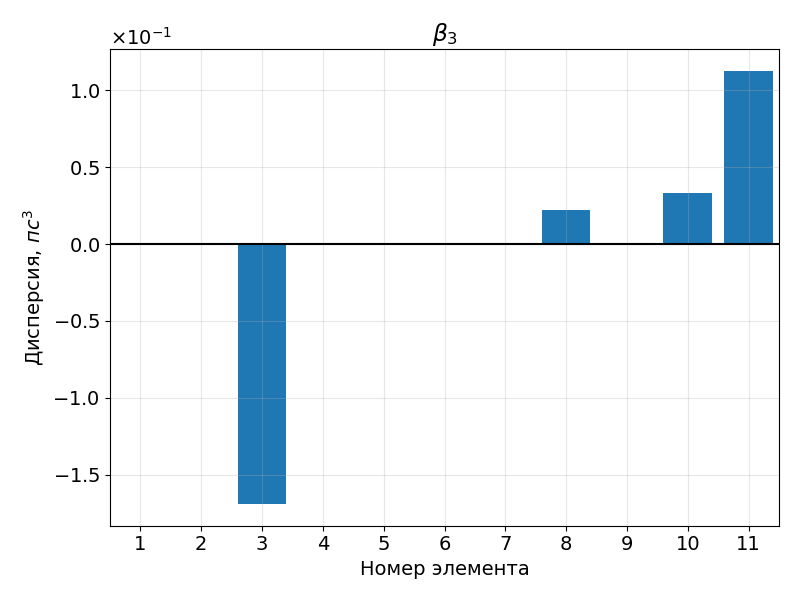
\includegraphics[width=\linewidth]{Images/Gauss Pulse x10/Беты/beta_3_full}
    \end{minipage}% <- % убирает хвостовой пробел / перевод строки
    \begin{minipage}[b]{0.5\textwidth}
        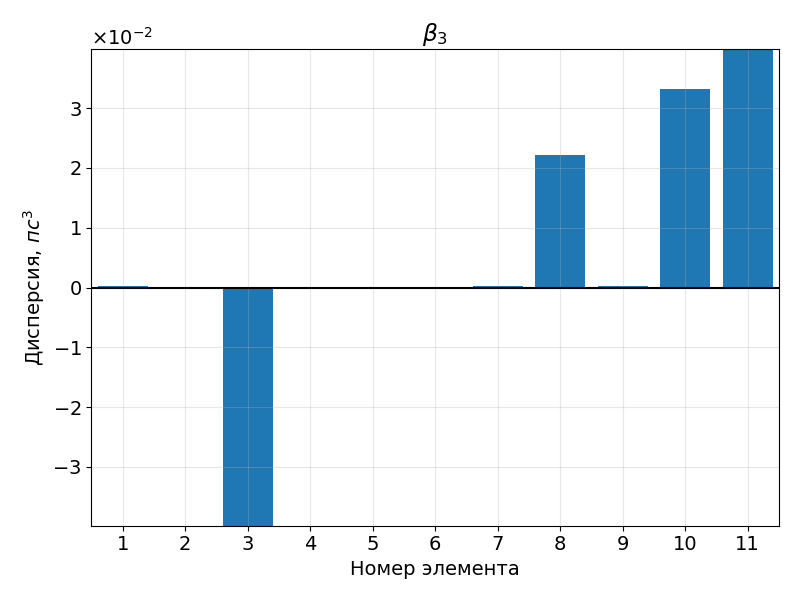
\includegraphics[width=\linewidth]{Images/Gauss Pulse x10/Беты/beta_3_cut}
    \end{minipage}

    \caption{Коэффициенты $\beta_3$, рассчитанные с помощью аппроксимации спектальной фазы полиномом,
     в двух масштабах (слева общий масштаб, справа увеличенный)}
    \label{fig:both}
\end{figure}

На рисунке 21 представлены графики для $\beta_4$. На них видно, что по абсолютному значению 8 элемент вносит самое
сильную модуляцию фазы. И этот порядок совершенно не компенсируется на компрессоре.

\begin{figure}[h!]
    \centering
    \begin{minipage}[b]{0.5\textwidth}
        \includegraphics[width=\linewidth]{Images/Gauss Pulse x10/Беты/beta_4_full}
    \end{minipage}% <- % убирает хвостовой пробел / перевод строки
    \begin{minipage}[b]{0.5\textwidth}
        \includegraphics[width=\linewidth]{Images/Gauss Pulse x10/Беты/beta_4_cut}
    \end{minipage}

    \caption{Коэффициенты $\beta_4$, рассчитанные с помощью аппроксимации спектальной фазы полиномом,
     в двух масштабах (слева общий масштаб, справа увеличенный)}
    \label{fig:both}
\end{figure}

На рисунке 22 представлены значения $B$-интеграла для каждого элемента схемы. Видно, что фазовая самомодуляция
на удлинённом волокне после второго каскада усиления имеет очень большое значение, почти $10\pi$ радиан.

\begin{figure}[h!]
    \centering
    \begin{minipage}[b]{0.5\textwidth}
        \includegraphics[width=\textwidth]{Images/Gauss Pulse x10/!B интегралы}
    \end{minipage}
    \caption{График $B$-интеграла на каждом элементе, изображённом в схеме установки на рисунке 2}
\end{figure}

\subsection{Моделирование схемы с укороченными волокнами}

Чтобы посмотреть, как изменится способность сжатия импульса при снижении фазовой самомодуляции, исключим 8 элемент
из схемы (рисунок 2). Именно на нём самый большой $B$-интеграл. На рисунке 23 представлен импульс после компрессора
(рисунок 23в) на выходе из оптической установки.

\begin{figure}[h!]
  \centering
  \begin{minipage}[b]{0.5\textwidth}
    \includegraphics[width=\linewidth]{Images/Gauss Pulse without 15-19/!23. Fiber_pusle}
  \end{minipage}% <- % убирает хвостовой пробел / перевод строки
  \begin{minipage}[b]{0.5\textwidth}
    \includegraphics[width=\linewidth]{Images/Gauss Pulse without 15-19/!23. Fiber_spectrum}
  \end{minipage}

  \vspace{}

  \begin{minipage}[b]{0.5\textwidth}
    \includegraphics[width=\linewidth]{Images/Gauss Pulse without 15-19/23 элемент gamma=50.14203 l_g=0.39316 сжатие}
  \end{minipage}% <- % убирает хвостовой пробел / перевод строки
  \begin{minipage}[b]{0.5\textwidth}
    \includegraphics[width=\linewidth]{Images/Gauss Pulse without 15-19/!23. Fiber_time_delay}
  \end{minipage}

  \caption{Гауссов а) импульс, б) его спектр г) и групповая задержка после третьего иттербиевого волокна (номер 10 на
  рисунке 2) с реальным профилем усиления. Приведён график г) импульса, сжатого в решёточном компрессоре}
  \label{fig:both}
\end{figure}

На рисунках 24 и 25 представлены вклады элементов в $\beta_3$ и $\beta_4$ соответственно. Видно, что волокна вносят
очень маленький вклад относительно стретчера (элемент 3) и компрессора (элемент 11).

\begin{figure}[h!]
    \centering
    \begin{minipage}[b]{0.5\textwidth}
        \includegraphics[width=\linewidth]{Images/Gauss Pulse without 15-19/Беты/beta_3_full}
    \end{minipage}% <- % убирает хвостовой пробел / перевод строки
    \begin{minipage}[b]{0.5\textwidth}
        \includegraphics[width=\linewidth]{Images/Gauss Pulse without 15-19/Беты/beta_3_cut}
    \end{minipage}

    \caption{Коэффициенты $\beta_3$, рассчитанные с помощью аппроксимации спектальной фазы полиномом,
     в двух масштабах (слева общий масштаб, справа увеличенный)}
    \label{fig:both}
\end{figure}

\begin{figure}[H]
    \centering
    \begin{minipage}[b]{0.5\textwidth}
        \includegraphics[width=\linewidth]{Images/Gauss Pulse without 15-19/Беты/beta_4_full}
    \end{minipage}% <- % убирает хвостовой пробел / перевод строки
    \begin{minipage}[b]{0.5\textwidth}
        \includegraphics[width=\linewidth]{Images/Gauss Pulse without 15-19/Беты/beta_4_cut}
    \end{minipage}

    \caption{Коэффициенты $\beta_4$, рассчитанные с помощью аппроксимации спектальной фазы полиномом,
     в двух масштабах (слева общий масштаб, справа увеличенный)}
    \label{fig:both}
\end{figure}

\clearpage
\section{Выводы}

Промоделирован волоконный трёхкаскадный усилитель чирпированных импульсов, длительность импульса
после компрессии для спектра усиления $Yb^{3+}$ составила 205 фс, энергия 1.037 мкДж, пъедестал импульса содержит
14\% энергии. Для импульса с параболическим профилем усиления длительность составила 207 фс, а энергия в пъедестале
1.6\%.

Основным физическим фактором, ограничивающим качество импульса после его компрессии, является фазовая самомодуляция.
При увеличении $B$-интеграла после второго каскада усилителя почти до 30 радиан длительность сжатого
импульса составила 235 фс, а энергия в пъедестале и пост- и предымпульсах составила 47\% от энергии импульса.
При уменьшении B-интеграла до 0 в этом же месте, длительность составила 192 фс. При этом энергия в пъедестале примерно 10\%.

Наклон в спектре усиления $Yb^{3+}$ ведёт к асимметрии во временной и спектральной формах импульса, что отражается
в увеличении энергии в его пъедестале от 1.6\% при параболическом профиле спектра усиления до 14\% для спектра
усиления иттербия.

\clearpage
\bibliographystyle{unsrt}
\bibliography{bibliography_references}

\end{document}
